\ifdefined\ishandout
\documentclass[handout]{beamer}
\else
\documentclass{beamer}
\fi

\usepackage[frenchb]{babel}
\usepackage[T1]{fontenc}
\usepackage[latin1]{inputenc}
\usepackage{hyperref}
\usepackage{multirow}
\usepackage{listings}
\usepackage{fancyvrb}
\usepackage{tikz}
\usepackage{framed}
\usepackage{algorithm}
\usepackage{algorithmic}
\usepackage{xcolor}
\usepackage{booktabs}
\usepackage{color, colortbl}
\ifdefined\ishandout
\usepackage{handoutWithNotes}
\fi
\usepackage{slashbox}
\usepackage{amsmath}
\usepackage{bm}
\usepackage{hhline}

\usetikzlibrary{shapes.geometric}
\usetikzlibrary{positioning}
\usetikzlibrary{shapes.arrows, chains}
\usetikzlibrary{arrows,calc}
\usetikzlibrary{shapes.multipart}
\usepackage{array}
\usetheme{Boadilla}

\usefonttheme[onlymath]{serif}

\newcommand{\R}{\mathbb{R}}
\newcommand{\C}{\mathbb{C}}
\newcommand{\N}{\mathbb{N}}
\newcommand{\Z}{\mathbb{Z}}
\newcommand{\E}{\mathbb{E}}
\newcommand{\Var}{\text{Var}}
\newcommand{\Cov}{\text{Cov}}
\ifdefined\ishandout
\pgfpagesuselayout{3 on 1 with notes}[a4paper,border shrink=5mm]
\usecolortheme{dove}
\else
%\usecolortheme{dolphin}
\usecolortheme{beaver}
\fi


\lstnewenvironment{codeC}
{ \lstset{language=C,
    otherkeywords={printf,scanf}}
}
{}

\ifdefined\ishandout
\definecolor{mygreen}{rgb}{0,0,0}
\definecolor{mymauve}{rgb}{0,0,0}
\definecolor{myblue}{rgb}{0,0,0}
\else
\definecolor{mygreen}{rgb}{0,0.6,0}
\definecolor{mymauve}{rgb}{0.58,0,0.82}
\definecolor{myblue}{rgb}{0,0,1}

\fi

%% Notes
%\setbeameroption{show only notes}


\definecolor{mygray}{rgb}{0.5,0.5,0.5}

\lstset{ language=Python,%
  backgroundcolor=\color{white},   % choose the background color; you must add \usepackage{color} or \usepackage{xcolor}
  basicstyle=\footnotesize,        % the size of the fonts that are used for the code
  breakatwhitespace=false,         % sets if automatic breaks should only happen at whitespace
  breaklines=true,                 % sets automatic line breaking
  captionpos=b,                    % sets the caption-position to bottom
  commentstyle=\color{mygreen},    % comment style
  deletekeywords={...},            % if you want to delete keywords from the given language
  escapeinside={\%*}{*)},          % if you want to add LaTeX within your code
  extendedchars=true,              % lets you use non-ASCII characters; for 8-bits encodings only, does not work with UTF-8
  frame=tb,	                   % adds a frame around the code
  keepspaces=true,                 % keeps spaces in text, useful for keeping indentation of code (possibly needs columns=flexible)
  keywordstyle=\color{blue},       % keyword style
  otherkeywords={*,...},           % if you want to add more keywords to the set
  numbers=none,                    % where to put the line-numbers; possible values are (none, left, right)
  numbersep=5pt,                   % how far the line-numbers are from the code
  numberstyle=\tiny\color{mygray}, % the style that is used for the line-numbers
  rulecolor=\color{black},         % if not set, the frame-color may be changed on line-breaks within not-black text (e.g. comments (green here))
  showspaces=false,                % show spaces everywhere adding particular underscores; it overrides 'showstringspaces'
  showstringspaces=false,          % underline spaces within strings only
  showtabs=false,                  % show tabs within strings adding particular underscores
  stepnumber=2,                    % the step between two line-numbers. If it's 1, each line will be numbered
  stringstyle=\color{mymauve},     % string literal style
  tabsize=3,	                   % sets default tabsize to 2 spaces
  title=\lstname                   % show the filename of files included with \lstinputlisting; also try caption instead of title
}
%\lstset{language=Python,
% breakatwhitespace=false,         % sets if automatic breaks should only happen at whitespace
%  breaklines=true,                 % sets automatic line breaking
%  captionpos=b,                
%%commentstyle=\itshape\color{mymauve},
%%keywordstyle=\bfseries\color{myblue},
%numbers=left,                    % where to put the line-numbers; possible values are (none, left, right)
%  numbersep=8pt,                   % how far the line-numbers are from the code
%  numberstyle=\tiny\color{mygray}, % the style that is used for the line-numbers
%%  rulecolor=\color{black},         % if not set, the frame-color may be changed on line-breaks within not-black text (e.g. comments (green here))
%  showspaces=false,                % show spaces everywhere adding particular underscores; it overrides 'showstringspaces'
%%  showstringspaces=false,          % underline spaces within strings only
%  showtabs=false,                  % show tabs within strings adding particular underscores
%  stepnumber=2,                    % the step between two line-numbers. If it's 1, each line will be numbered
%%  stringstyle=\color{mygreen},     % string literal style
%  tabsize=2 
%}
\ifdefined\ishandout
\newcommand{\red}{\textbf}
\else
\newcommand{\red}{\textcolor{red}}
\fi
%\newcommand \emph
%Default size : 12.8 cm * 9.6 cm

\newcommand{\tmark}[1]{\tikz[remember picture, baseline=-.5ex]{\coordinate(#1);}}

\ifdefined\ishandout
\newenvironment<>{codeblock}[1]{%begin
  \setbeamercolor{block title}{fg=black,bg=lightgray!80}%
  \begin{block}{#1}}
  % \begin{codeC}}
  %  {\end{codeC}
{  
\end{block}}

\newenvironment<>{termblock}[1]{
    \setbeamercolor{block title}{fg=black,bg=lightgray!90}%
    \begin{block}{#1}
}
%     \begin{Verbatim}}
{%\end{Verbatim}
\end{block}
}

\definecolor{bluegreen}{RGB}{0,0,0}
%\definecolor{bluegreen}{rgb}{0,0.6,0.8}
\else

\newenvironment<>{codeblock}[1]{%begin
  \setbeamercolor{block title}{fg=darkgray,bg=yellow}%
  \begin{block}{#1}}
  % \begin{codeC}}
  %  {\end{codeC}
{  
\end{block}}

\newenvironment<>{termblock}[1]{
    \setbeamercolor{block title}{fg=white,bg=lightgray}%
    \begin{block}{#1}}
%     \begin{Verbatim}}
{%\end{Verbatim}
\end{block}
}

\definecolor{bluegreen}{RGB}{0,149,182}
%\definecolor{bluegreen}{rgb}{0,0.6,0.8}
\fi

%\newcommand{\output}[1]{
\setbeamertemplate{navigation symbols}{}
\newcommand{\bvrb}{\Verb[commandchars=£µ§,formatcom=\color{bluegreen}]}
\newcommand{\footvrb}{\footnotesize\Verb}
\newcommand{\vrbalert}[2][]{\visible<#1>{#2}}
%%% Commande pour les listes/arbres
\newcommand{\mvide}{\nodepart{one} \nodepart{two}}
\newcommand{\tvide}{\nodepart{one} \nodepart{two} \nodepart{three}}

%%Fin des commandes pour les listes/arbres.



%%% Paramètres du cours (à régler)
%Numéro du cours
\newcommand{\nb}{1}

\title[non-linear]{Toward non-linear regression/classification}
\author[non-linear]{julien.brajard@upmc.fr}
\institute[UPMC]{UPMC}
\date{1-5 August 2016}

\begin{document}
%%%%%%%%%%%%%%%%%%%%% SLIDES DE TITRE
\begin{frame}
\titlepage
%\centering{
%\url{http://australe.upmc.fr} (onglet EPU-C5-IGE Info Gen)}
\end{frame}
%%%%%%%%%%%%%%%%%%%%%
\begin{frame}
\frametitle{Polynomial regression}
model selection
learning/test/
validation
\end{frame}
\begin{frame}
\frametitle{Example of a non-linear relashionship}
\begin{figure}
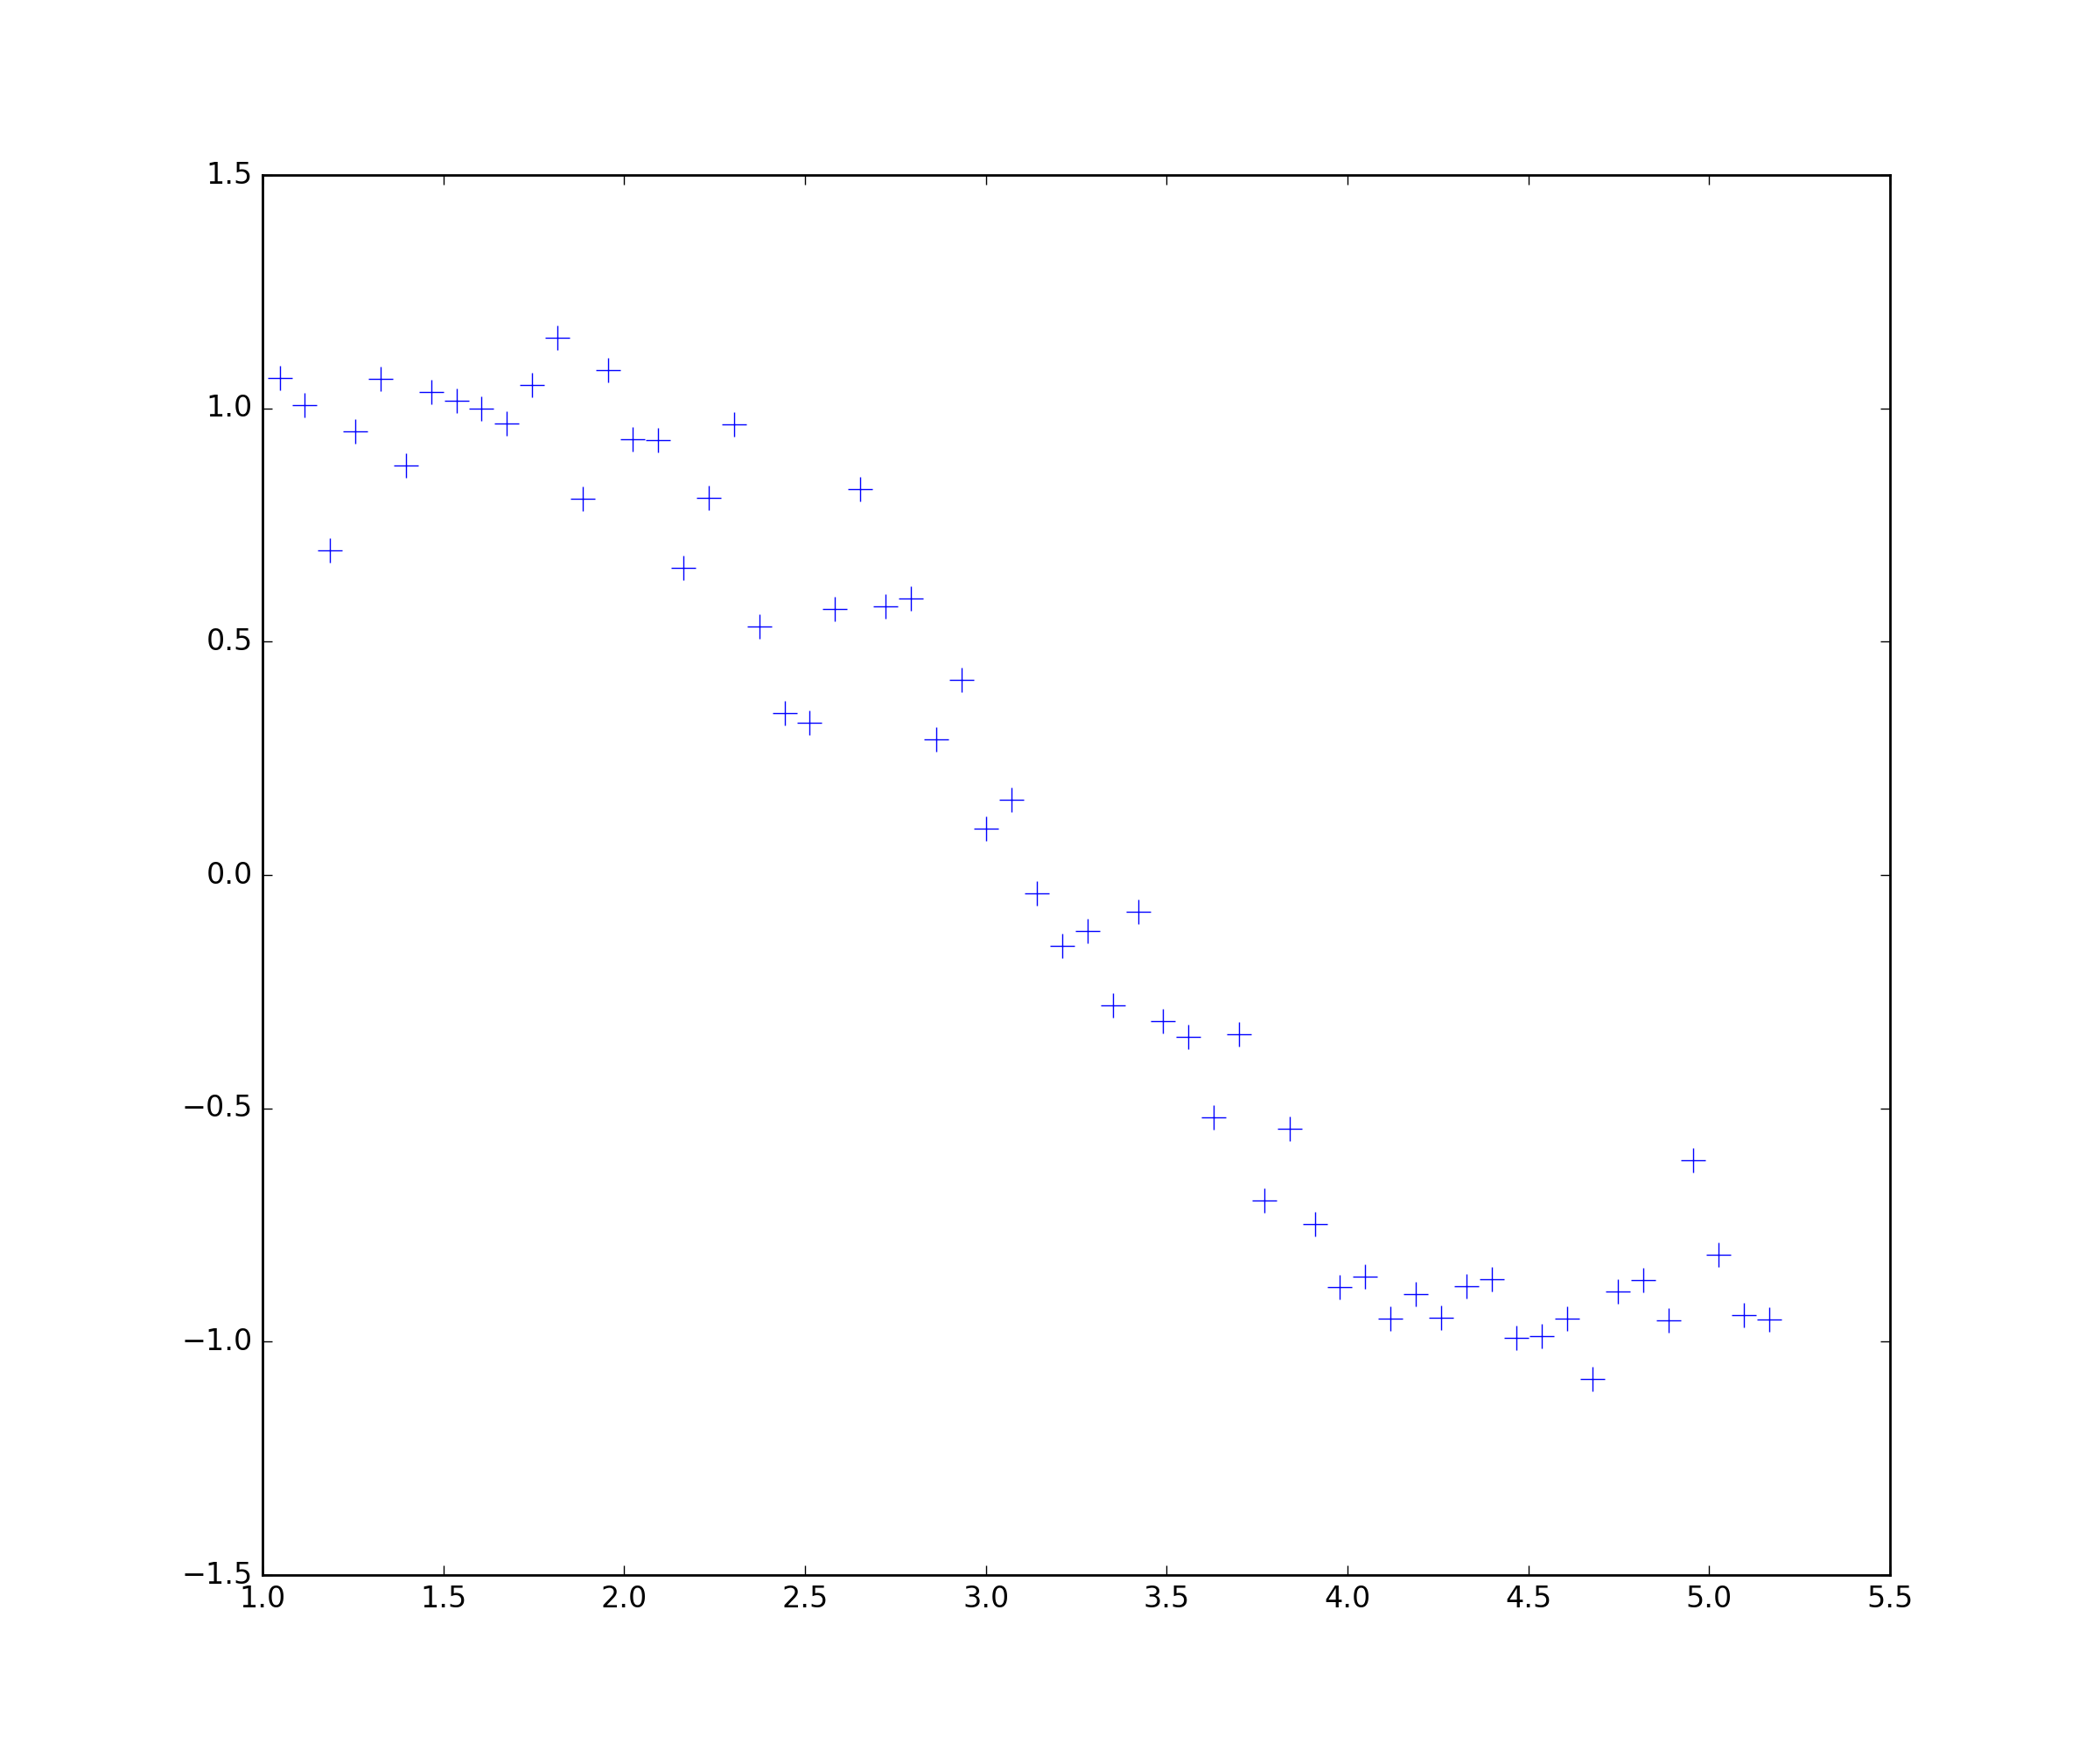
\includegraphics[height=0.55\textheight]{./fig/scatter.png}
\end{figure}
\begin{block}{An idea}
We could take an polynomial hypothesis model:
$$
h_{\bm{\theta}}(x) = \theta_0 x^0 + \theta_1 x^1 + \ldots + \theta_p x^p
$$
\end{block}
\end{frame}
%%%%%%%%%%%%%%%%%%%%%
\begin{frame}
\frametitle{Example}
$\{(x_1,y_1),\ldots,(x_n,y_n)\}$ is the learning dataset.

For a given polynom degree $p$, parameters $\bm{\theta}$ are determined minimizing the 
least-mean square cost function:
$$
J(\bm{\theta}) = \frac{1}{n} \sum (y_i - h_{\bm{\theta}}(x_i))^2
$$
with $h_{\bm{\theta}}(x) = \theta_0 x^0 + \theta_1 x^1 + \ldots + \theta_p x^p$
\begin{itemize}[<+->]
\item It can be determined using a gradient descent method
\item If the degree of the polynom $p=1$, it is a simple linear regression
\end{itemize}
\end{frame}
%%%%%%%%%%%%%%%%%%%%%
\begin{frame}
\frametitle{A first result}
\vspace{-2em}
\begin{columns}[t]
\column{.5\textwidth}
\begin{figure}
$p=1$ (linear regression)\\
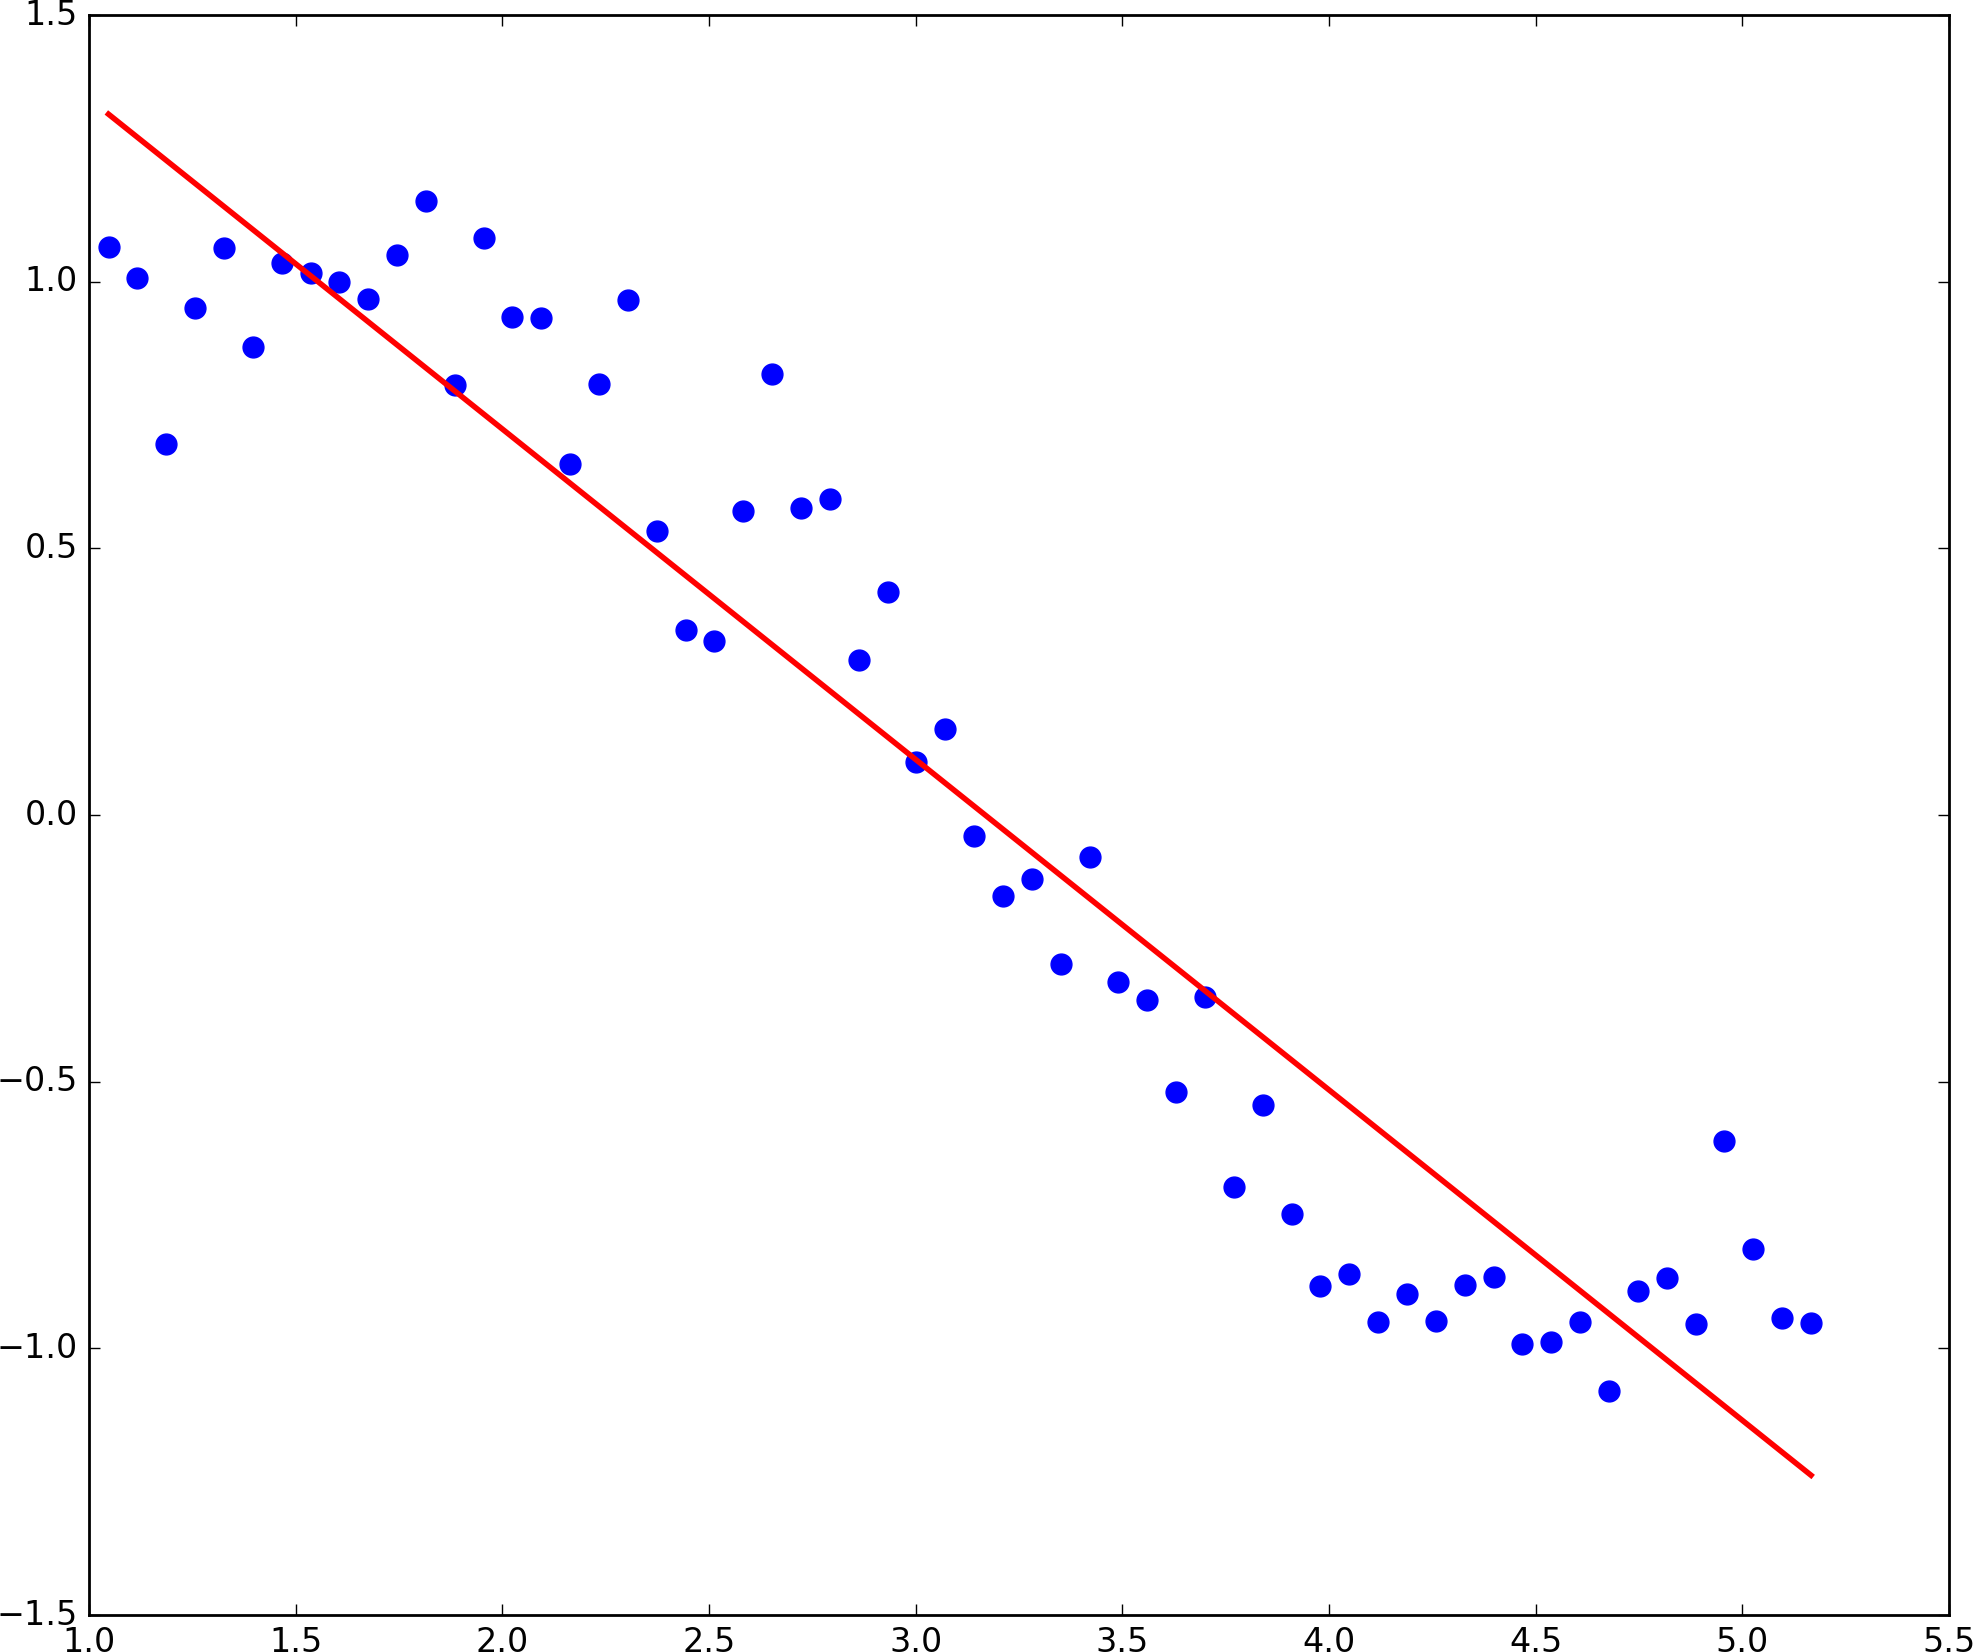
\includegraphics[width=0.99\textwidth]{./fig/linreg_pow1.png}
\end{figure}
\column{.5\textwidth}
\begin{figure}
residuals\\
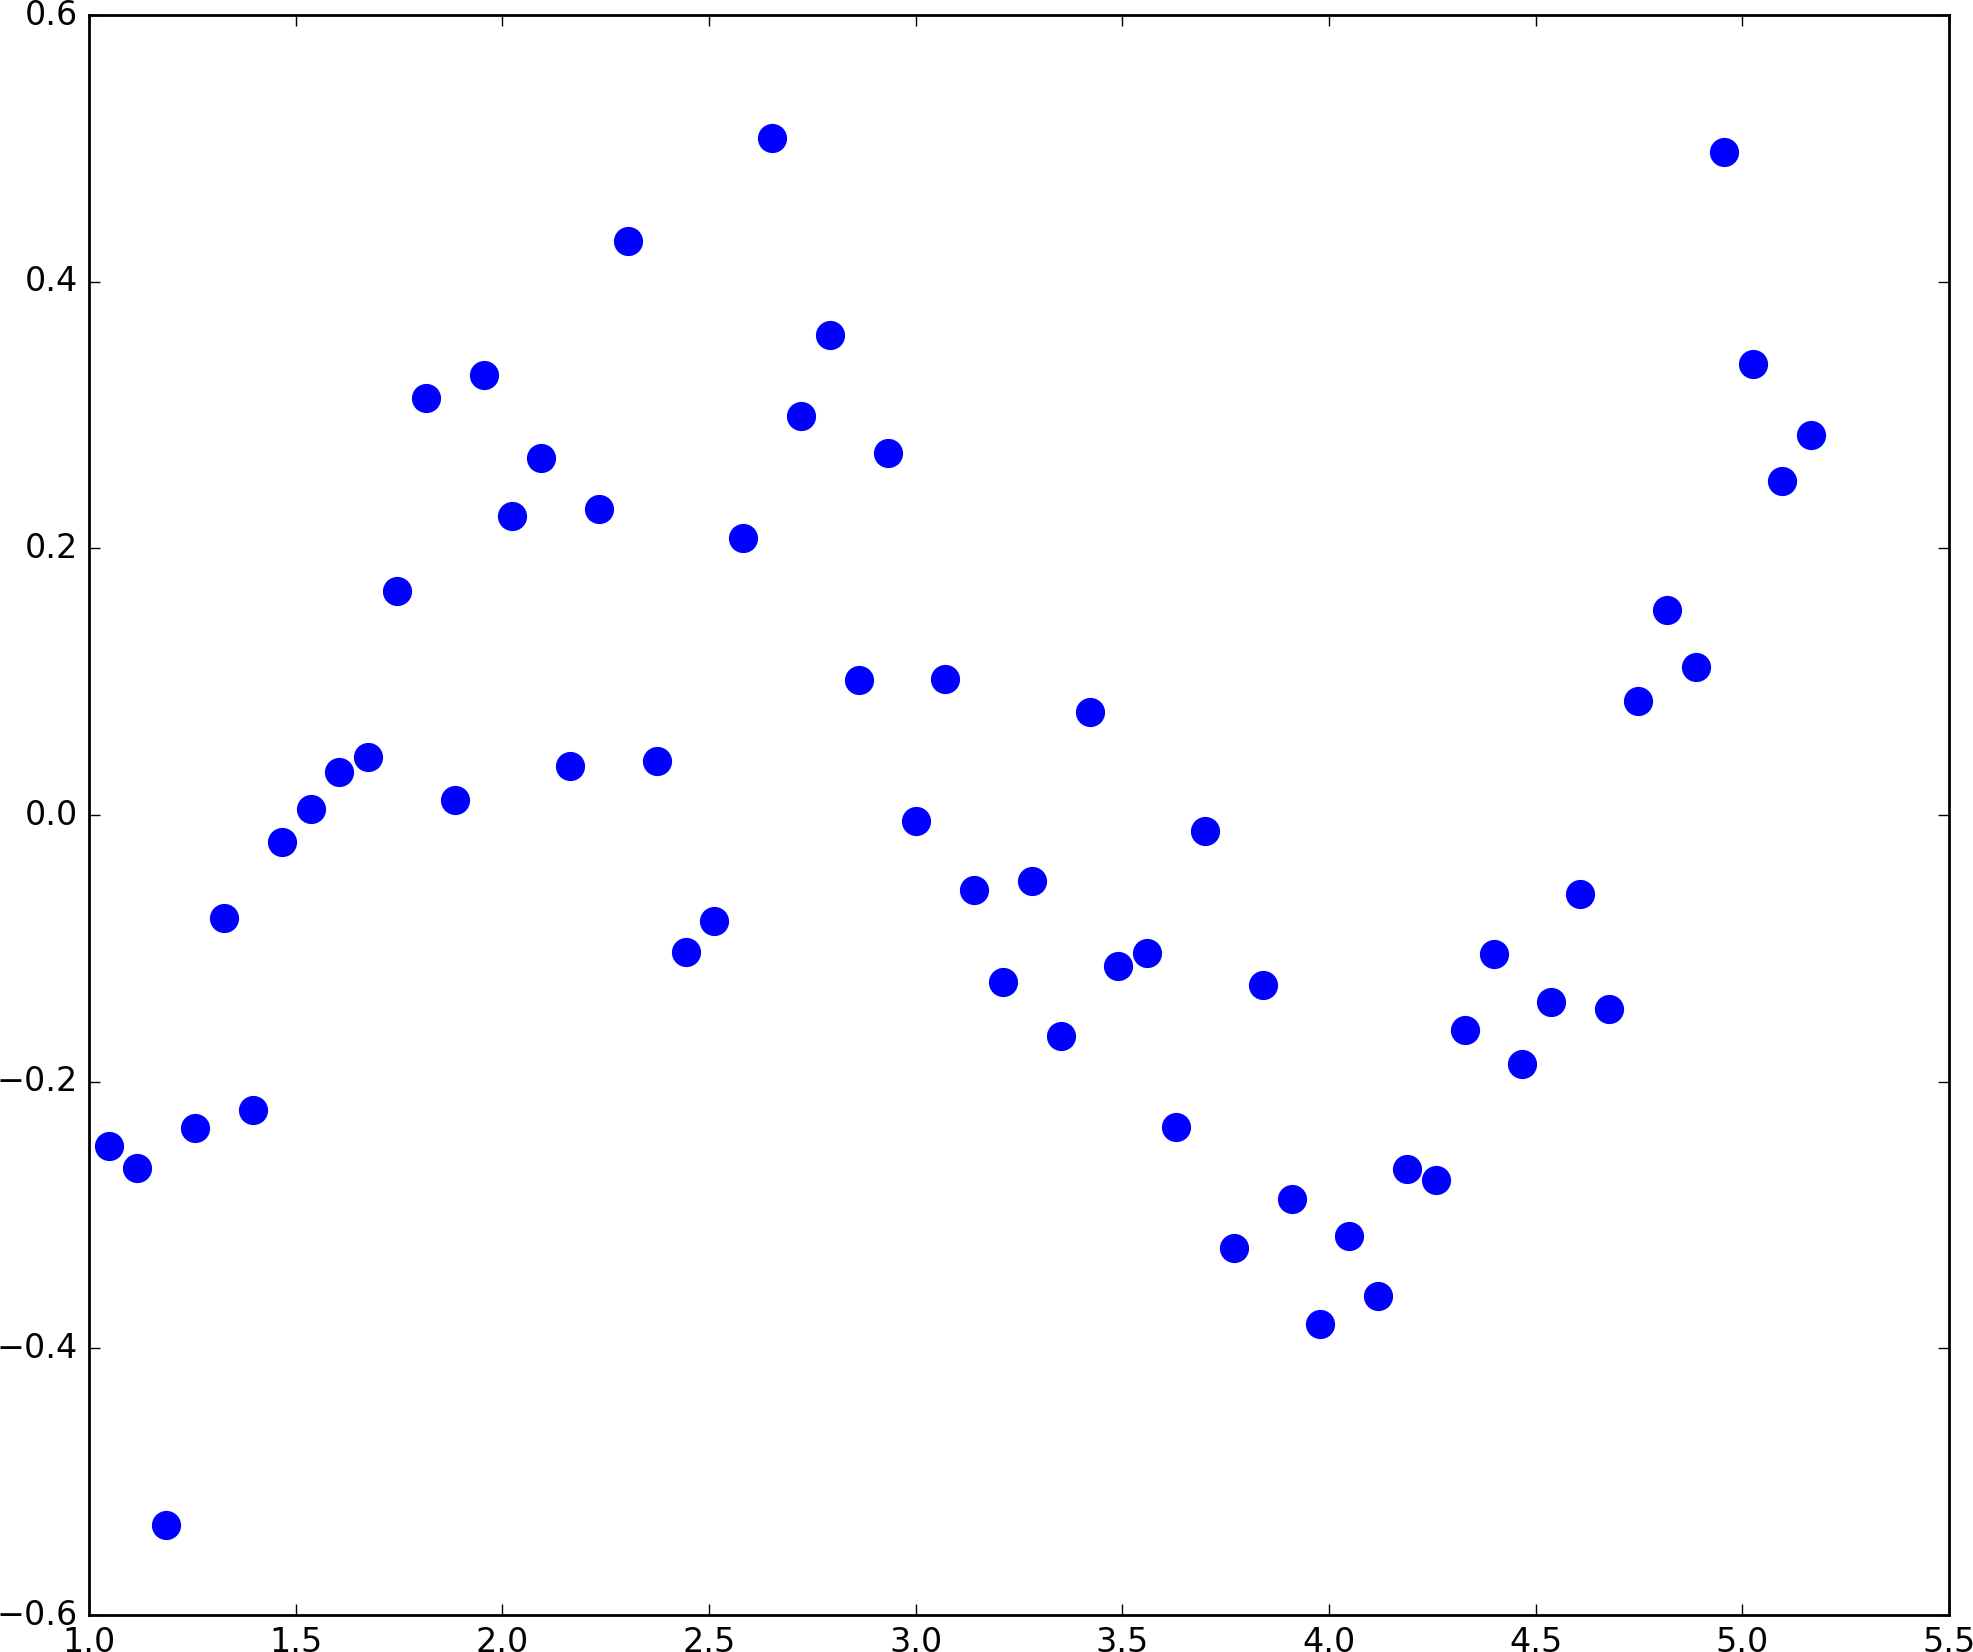
\includegraphics[width=0.99\textwidth]{./fig/residuals.png}
\end{figure}

\end{columns}
\begin{block}{Prediction error}
$$
\text{err} = \frac{1}{n}\sum \text{res}^2 = 5.46e-2
$$
\end{block}

\end{frame}
%%%%%%%%%%%%%%%%%%%%%
\begin{frame}
\frametitle{Increasing the polynomial degree ?}
\begin{columns}
\column{.5\textwidth}
\begin{figure}
$p=3$ (cubic regression)\\
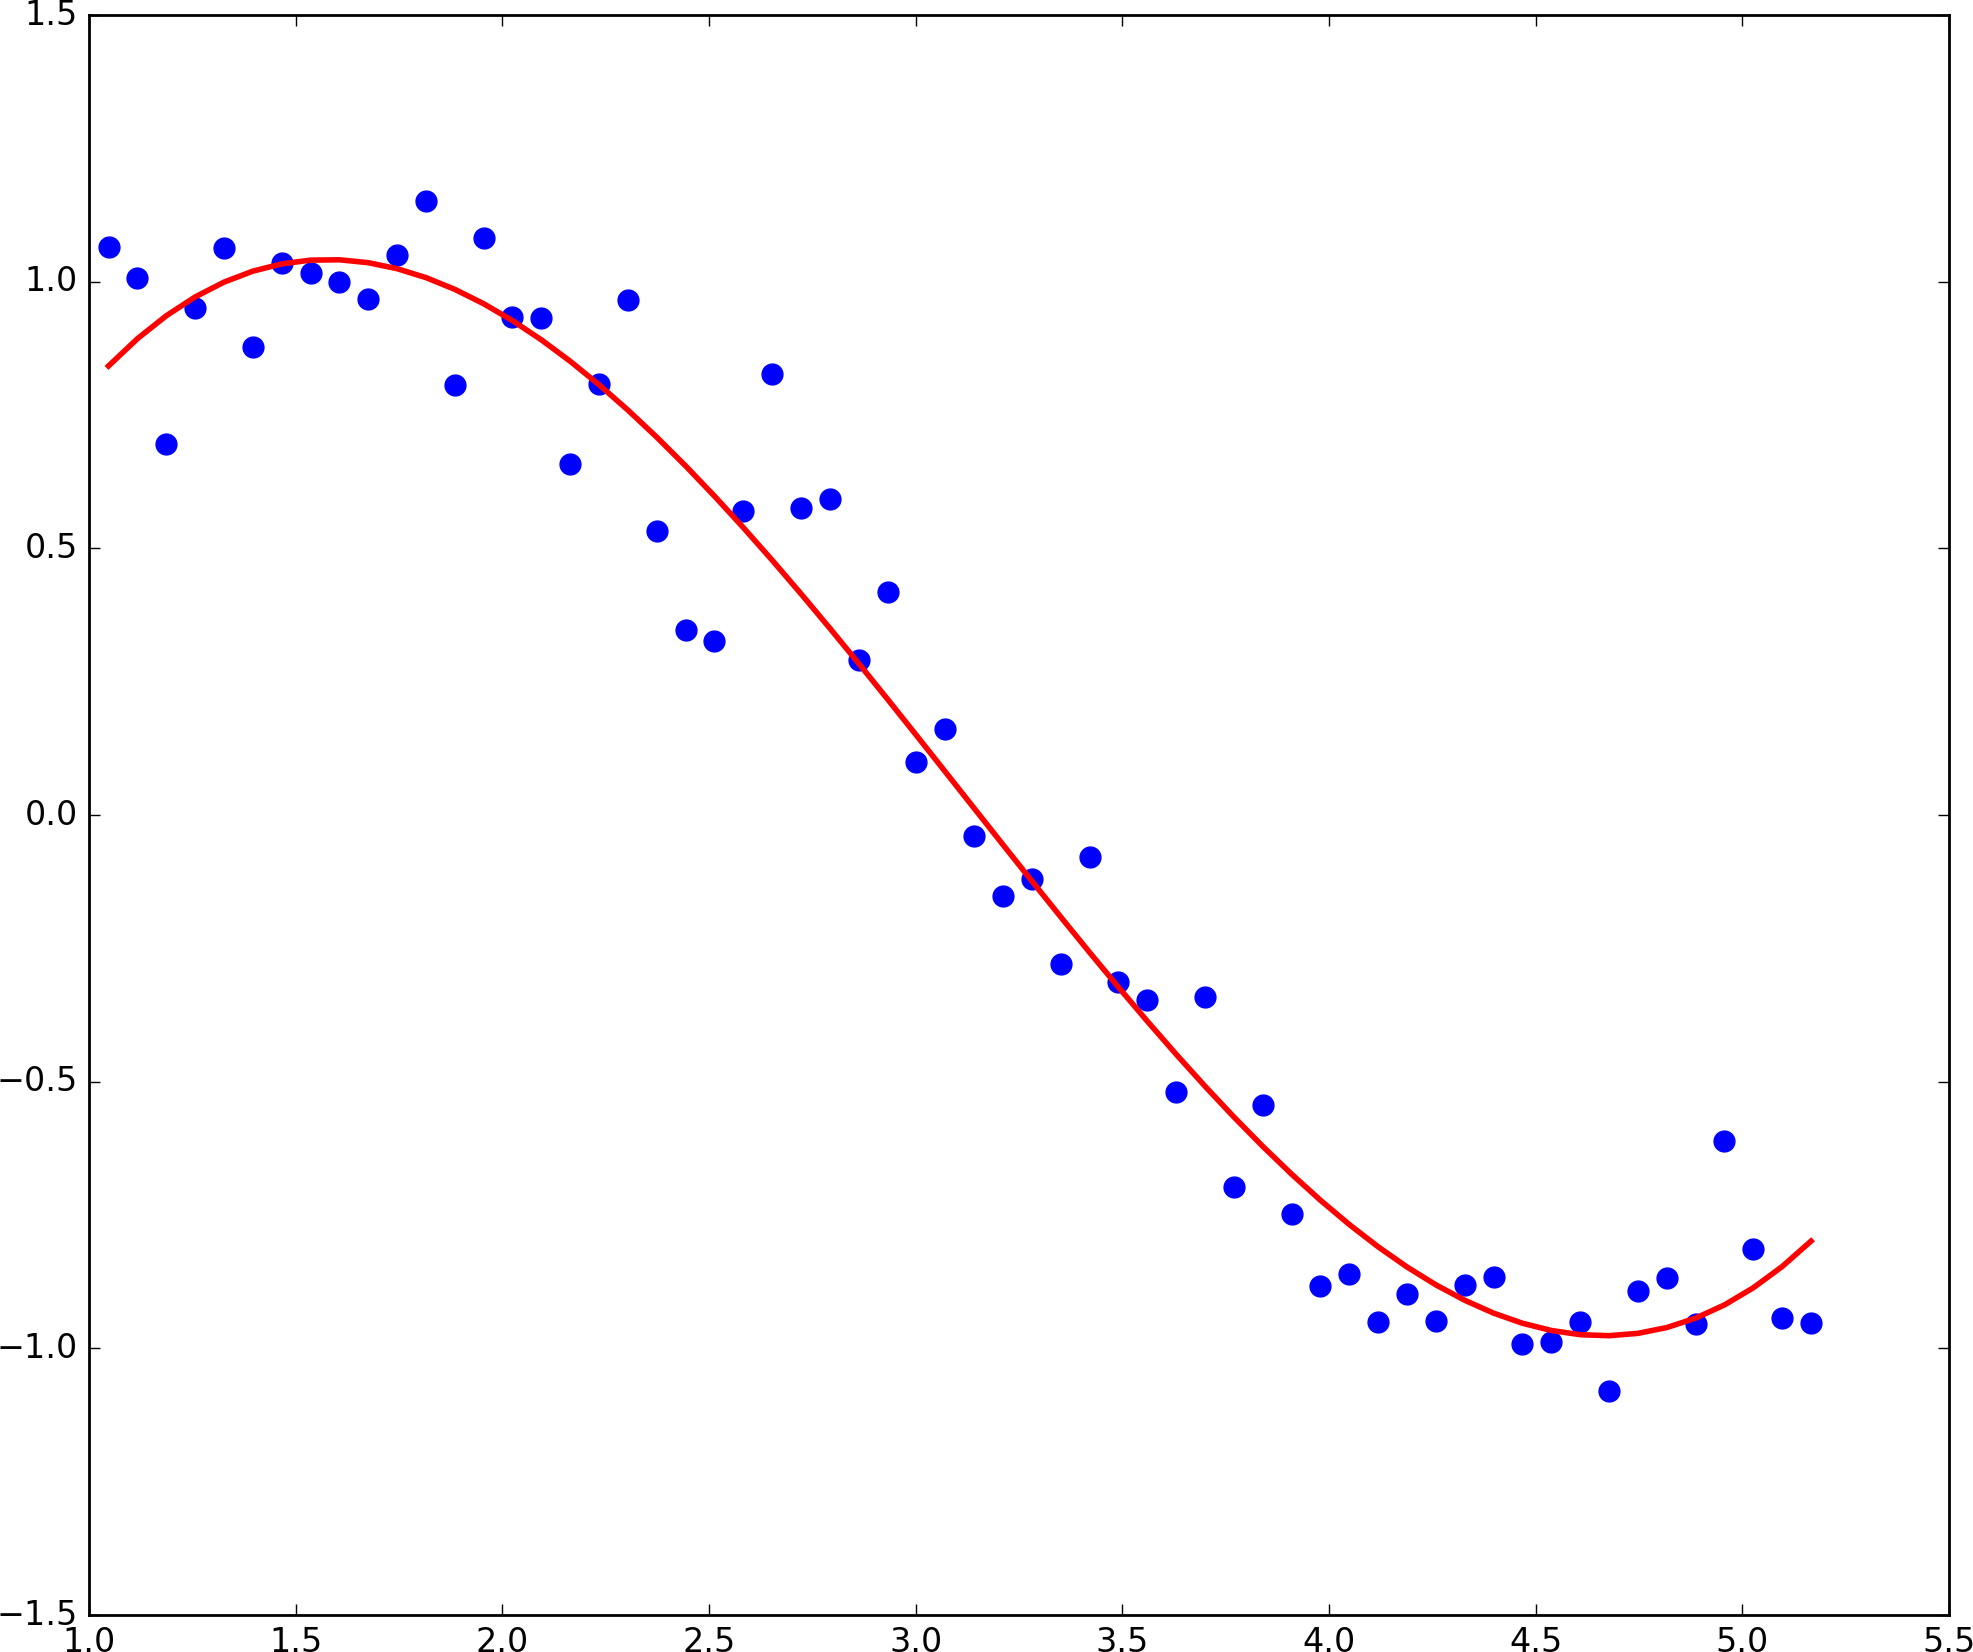
\includegraphics[width=0.99\textwidth]{./fig/linreg_pow3.png}
\end{figure}
\column{.5\textwidth}
\begin{block}{Prediction error}
$$
\text{err} = \frac{1}{n}\sum \text{res}^2 = 1.80e-2
$$
\end{block}
\end{columns}
\end{frame}


%%%%%%%%%%%%%%%%%%%%%
\begin{frame}
\frametitle{Is it different from the linear regression ?}
Let's consider :
$$
\bm{x} = 
\begin{pmatrix}
1 \\
x^1 \\
x^2 \\
\vdots \\
x^p
\end{pmatrix}
$$
then
$$
h_{\bm{\theta}}(x) = \theta_0  + \theta_1 x^1 + \ldots + \theta_p x^p = \bm{\theta}^T \bm{x}
$$
\begin{alertblock}{}
By extending a scalar predictor to a vector,
polynomial regression is equivalent to linear regression.
\end{alertblock}

\end{frame}

%%%%%%%%%%%%%%%%%%%%%
\begin{frame}
\frametitle{Increasing the degree ?}
\begin{columns}
\column{.33\textwidth}
\vspace{-2em}
\begin{figure}
$p=1$
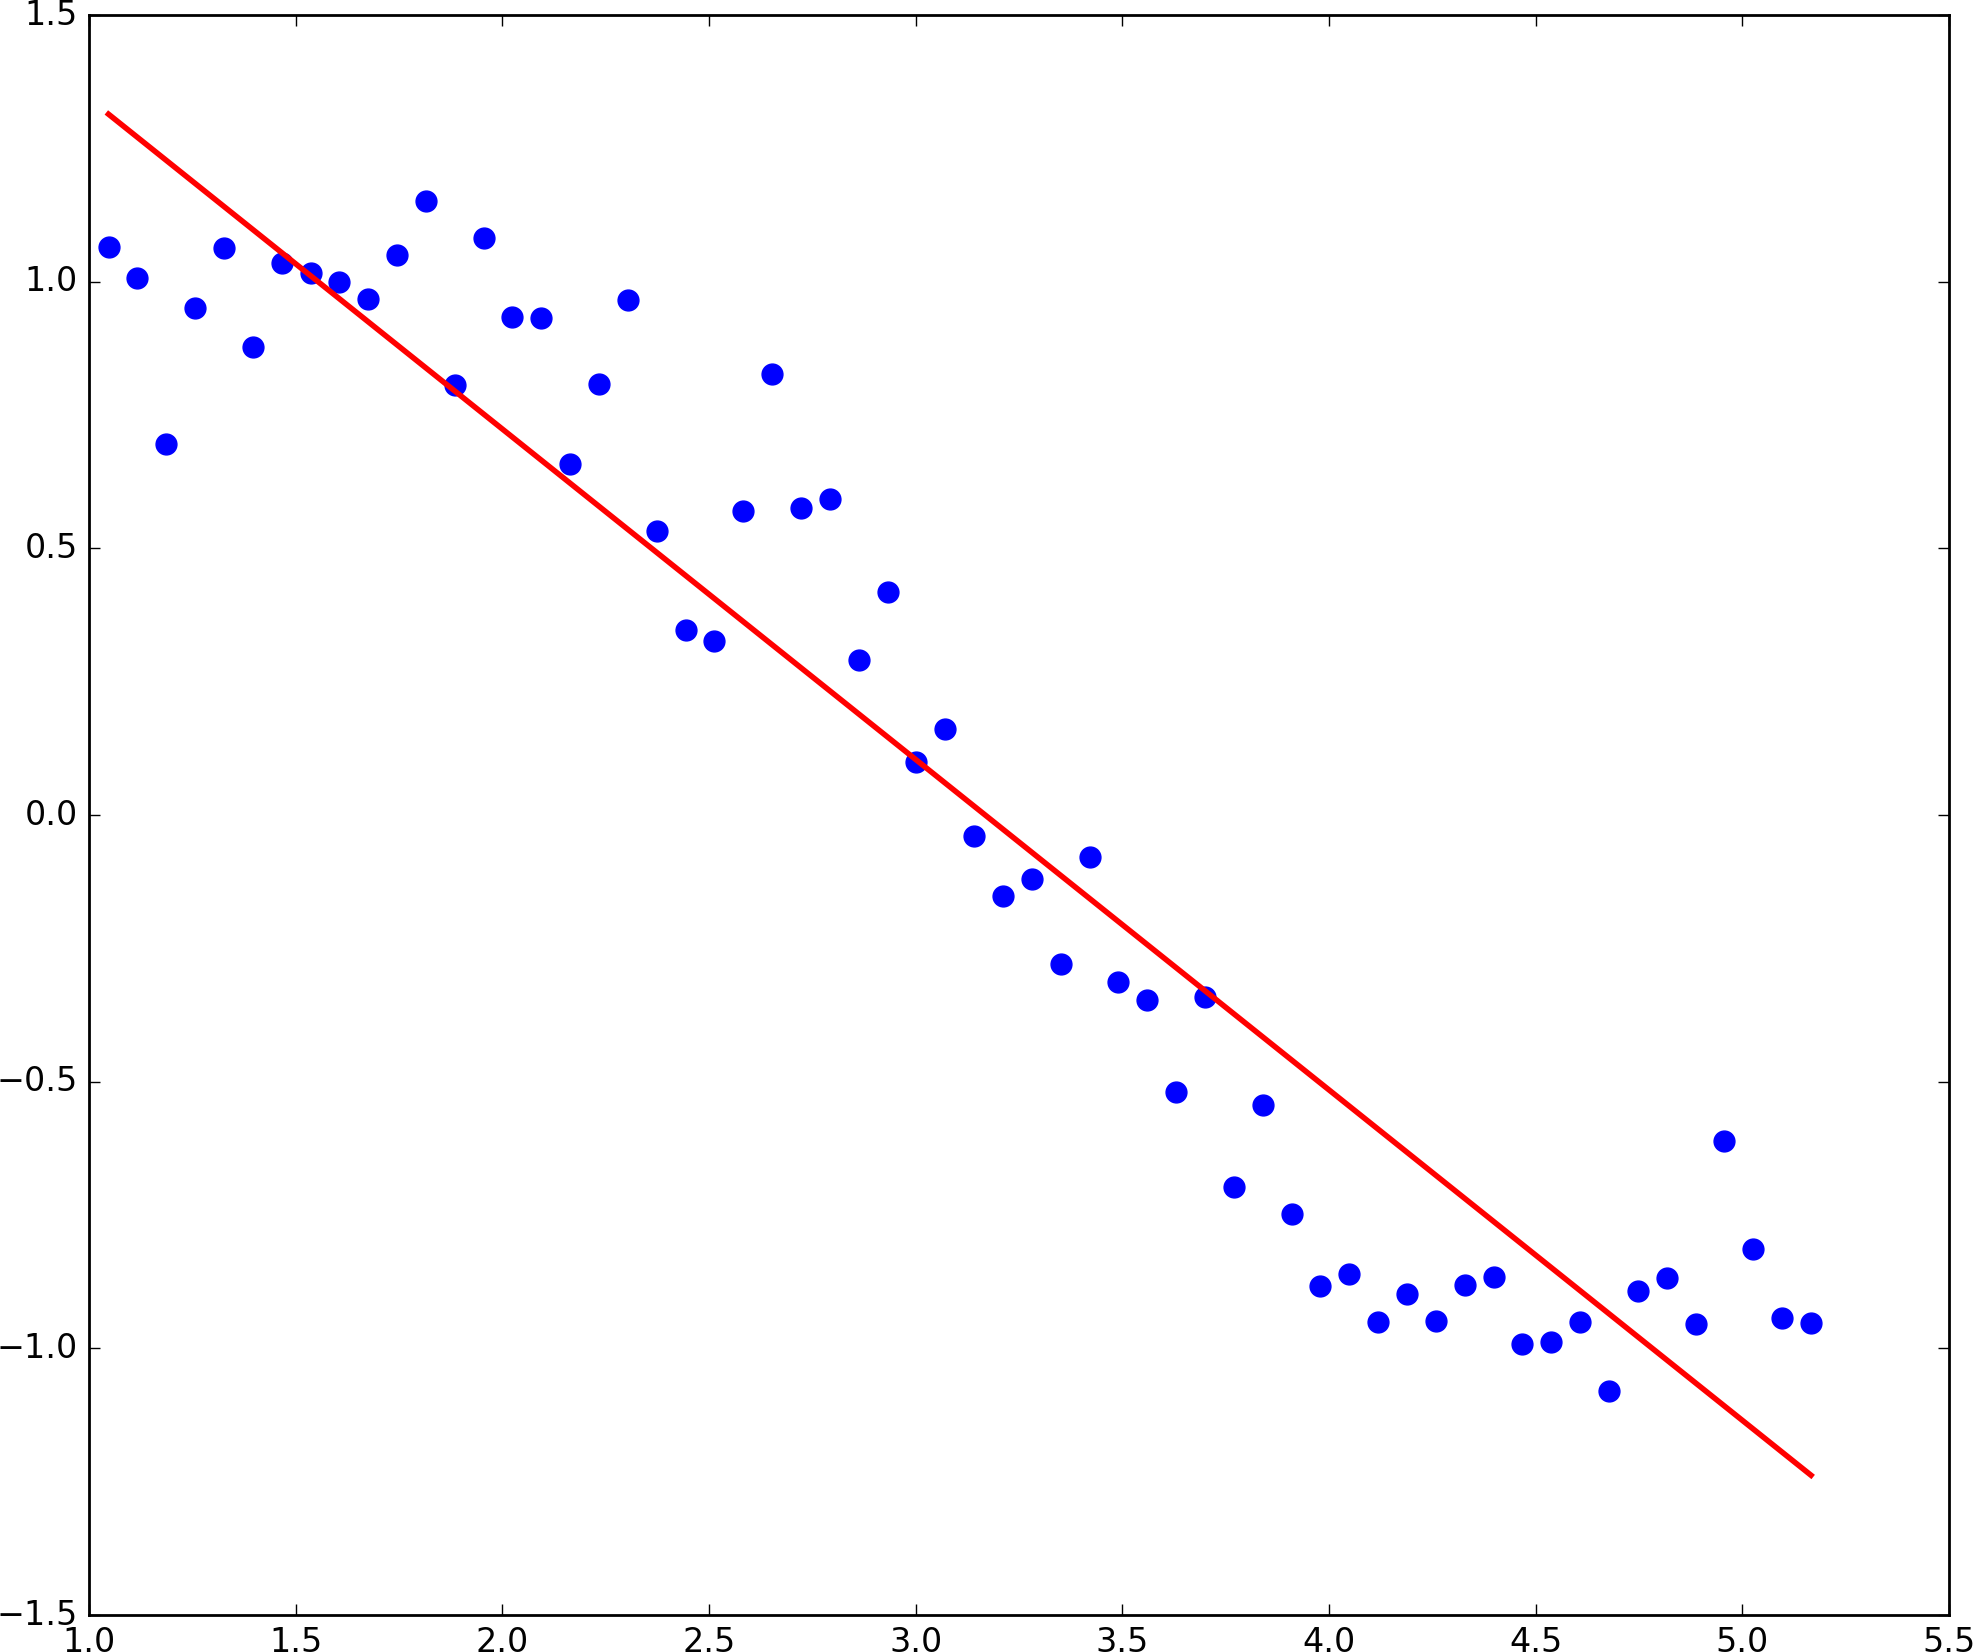
\includegraphics[width=0.99\textwidth]{./fig/linreg_pow1.png}
\end{figure}
\vspace{-2em}
\begin{figure}
$p=9$
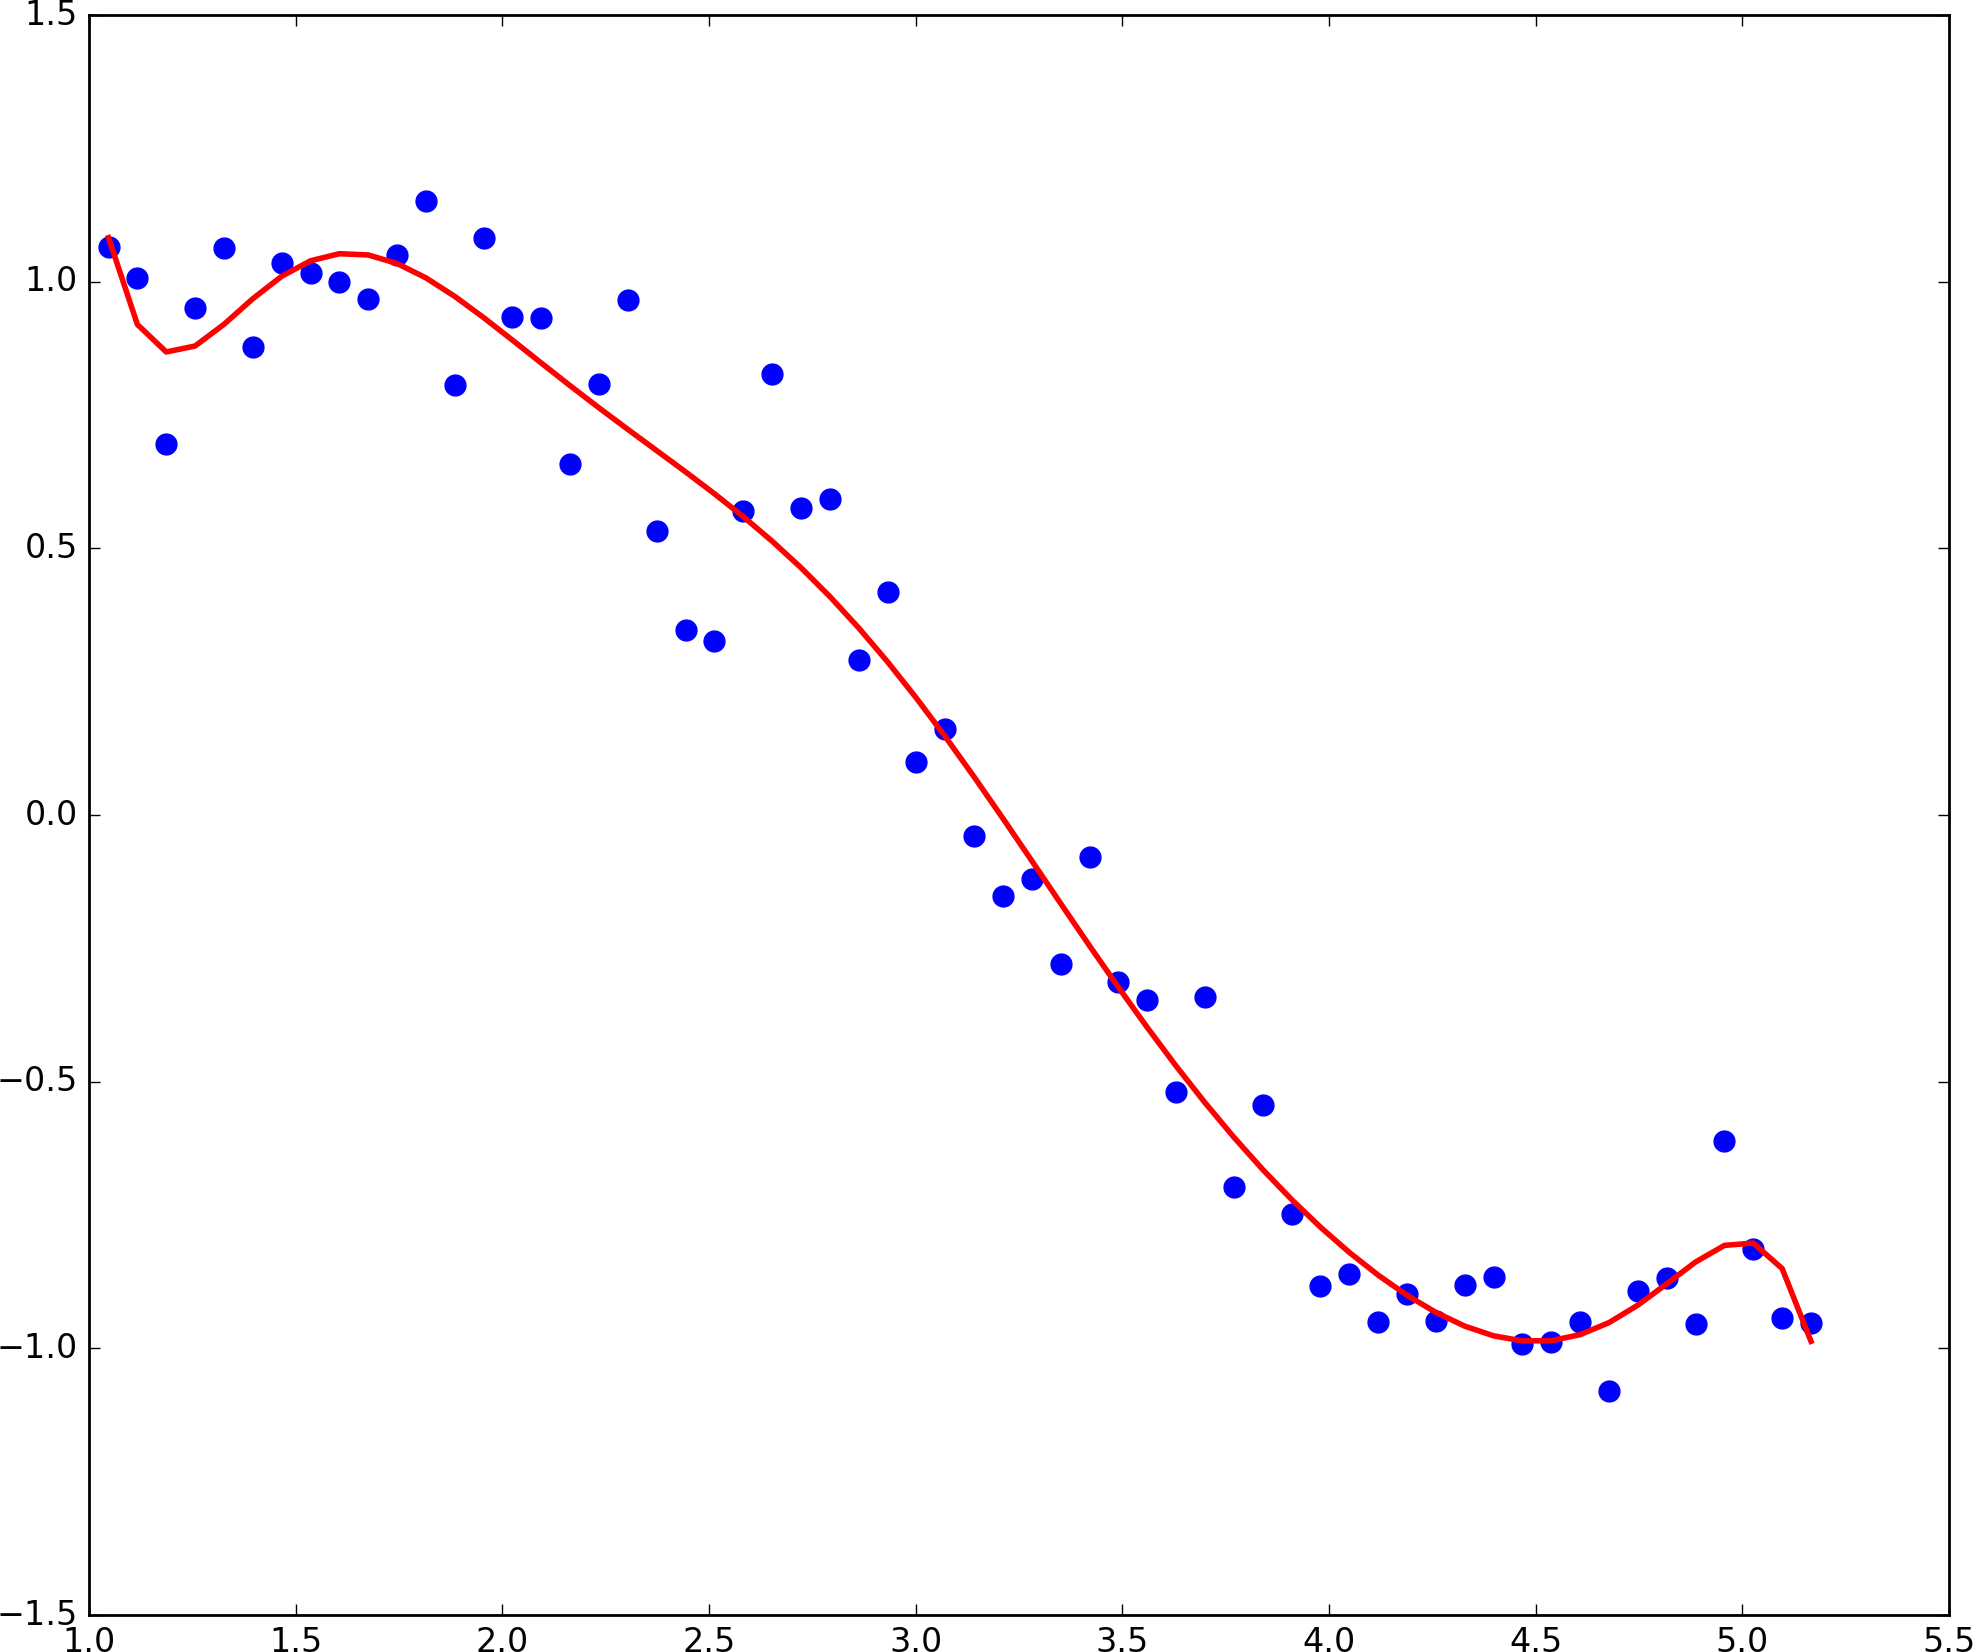
\includegraphics[width=0.99\textwidth]{./fig/linreg_pow9.png}
\end{figure}
\column{.33\textwidth}
\vspace{-2em}
\begin{figure}
$p=3$
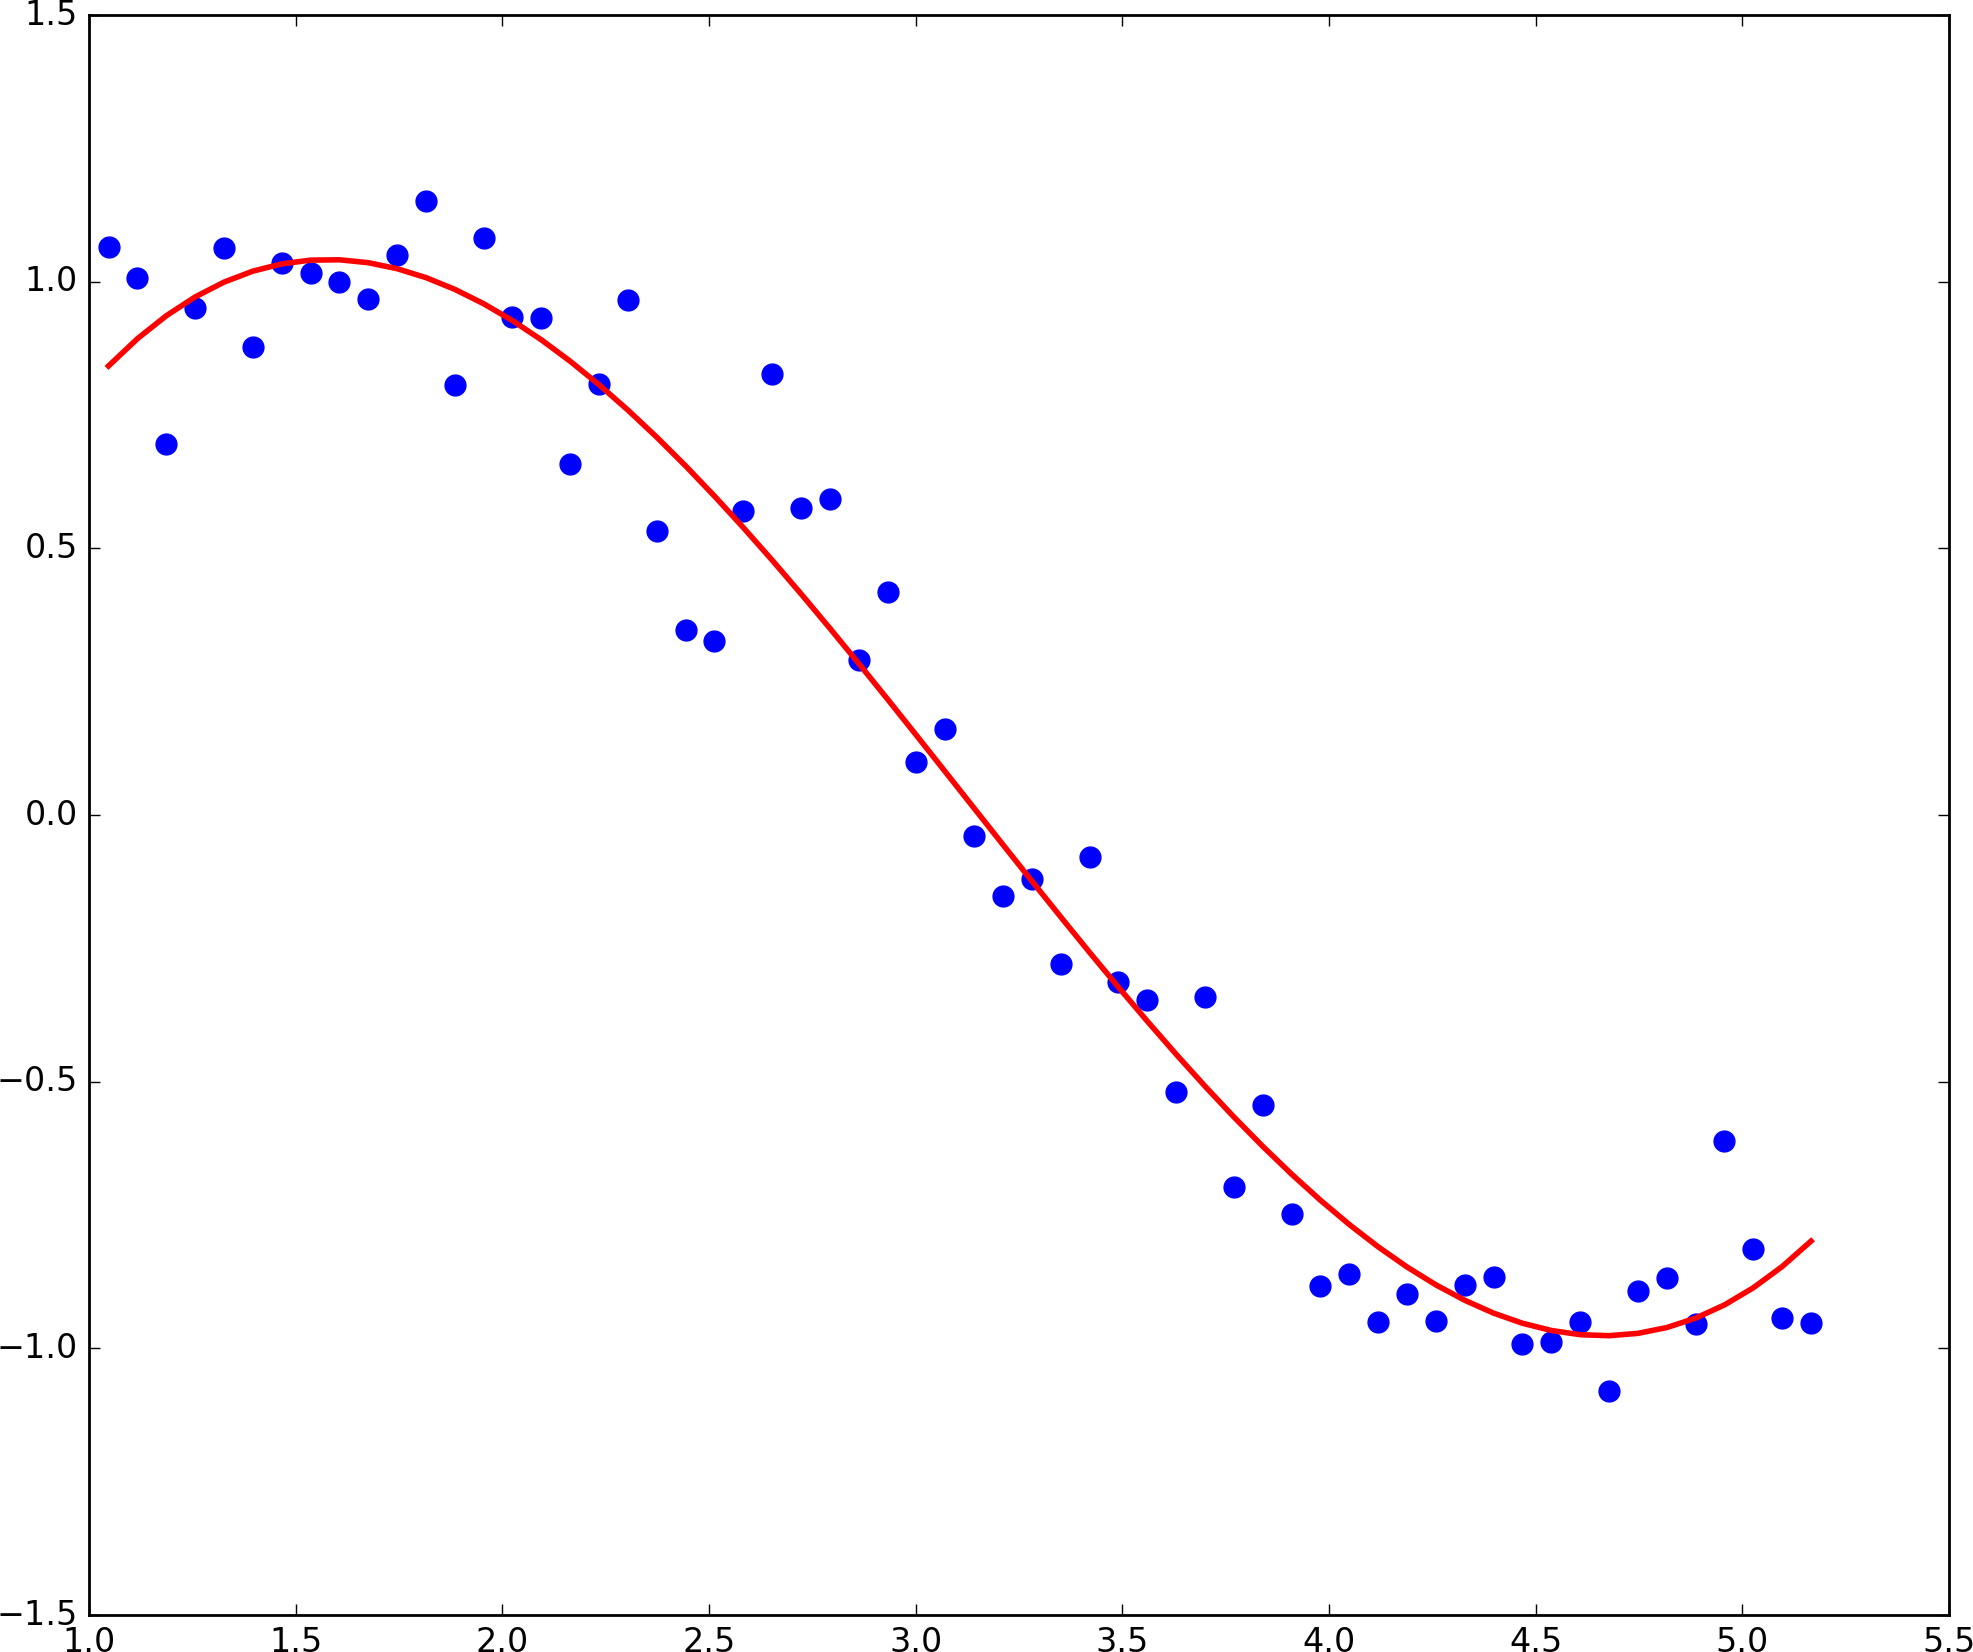
\includegraphics[width=0.99\textwidth]{./fig/linreg_pow3.png}
\end{figure}
\vspace{-2em}
\begin{figure}
$p=12$
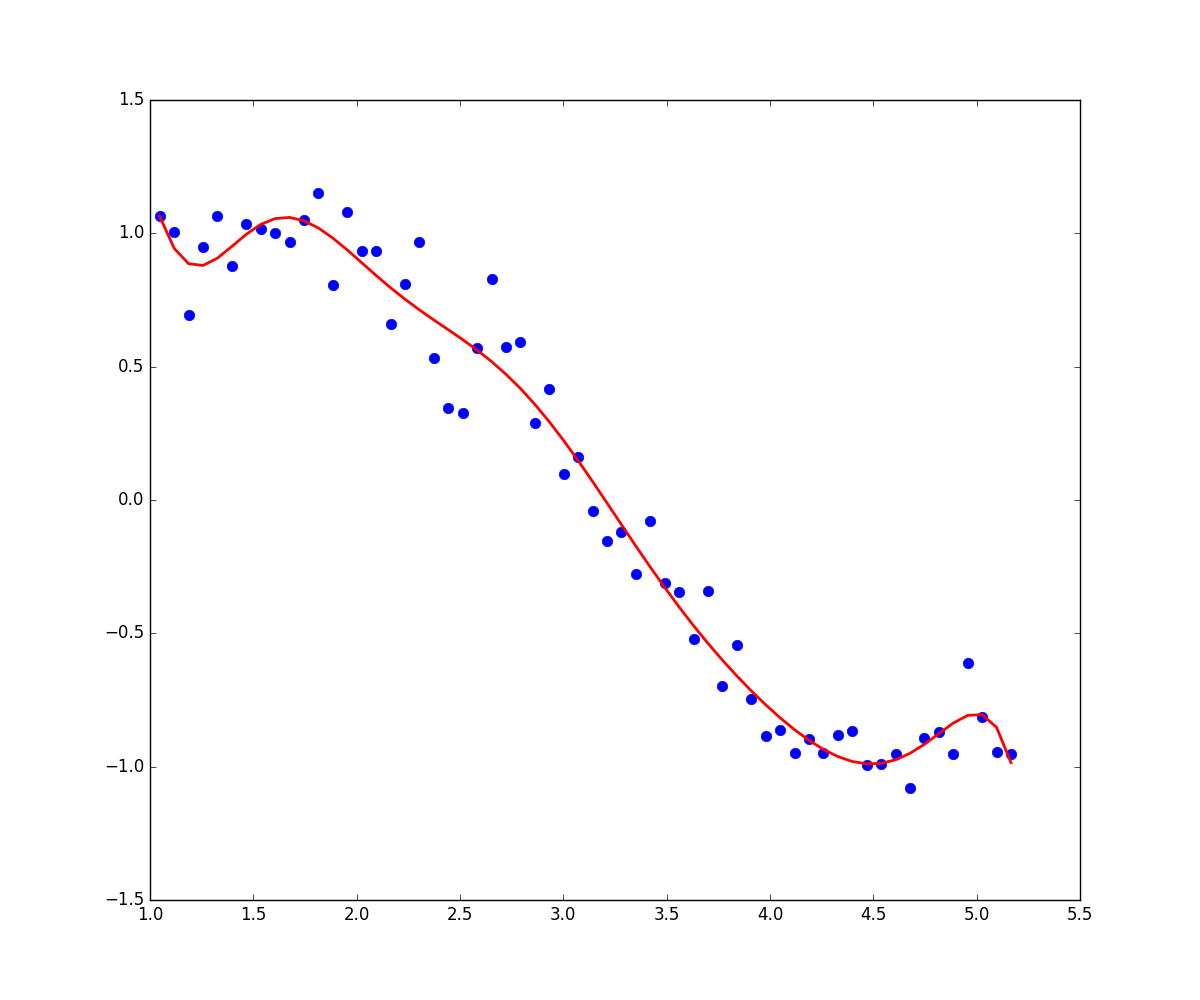
\includegraphics[width=0.99\textwidth]{./fig/linreg_pow12.png}
\end{figure}
\column{.33\textwidth}
\vspace{-2em}
\begin{figure}
$p=4$
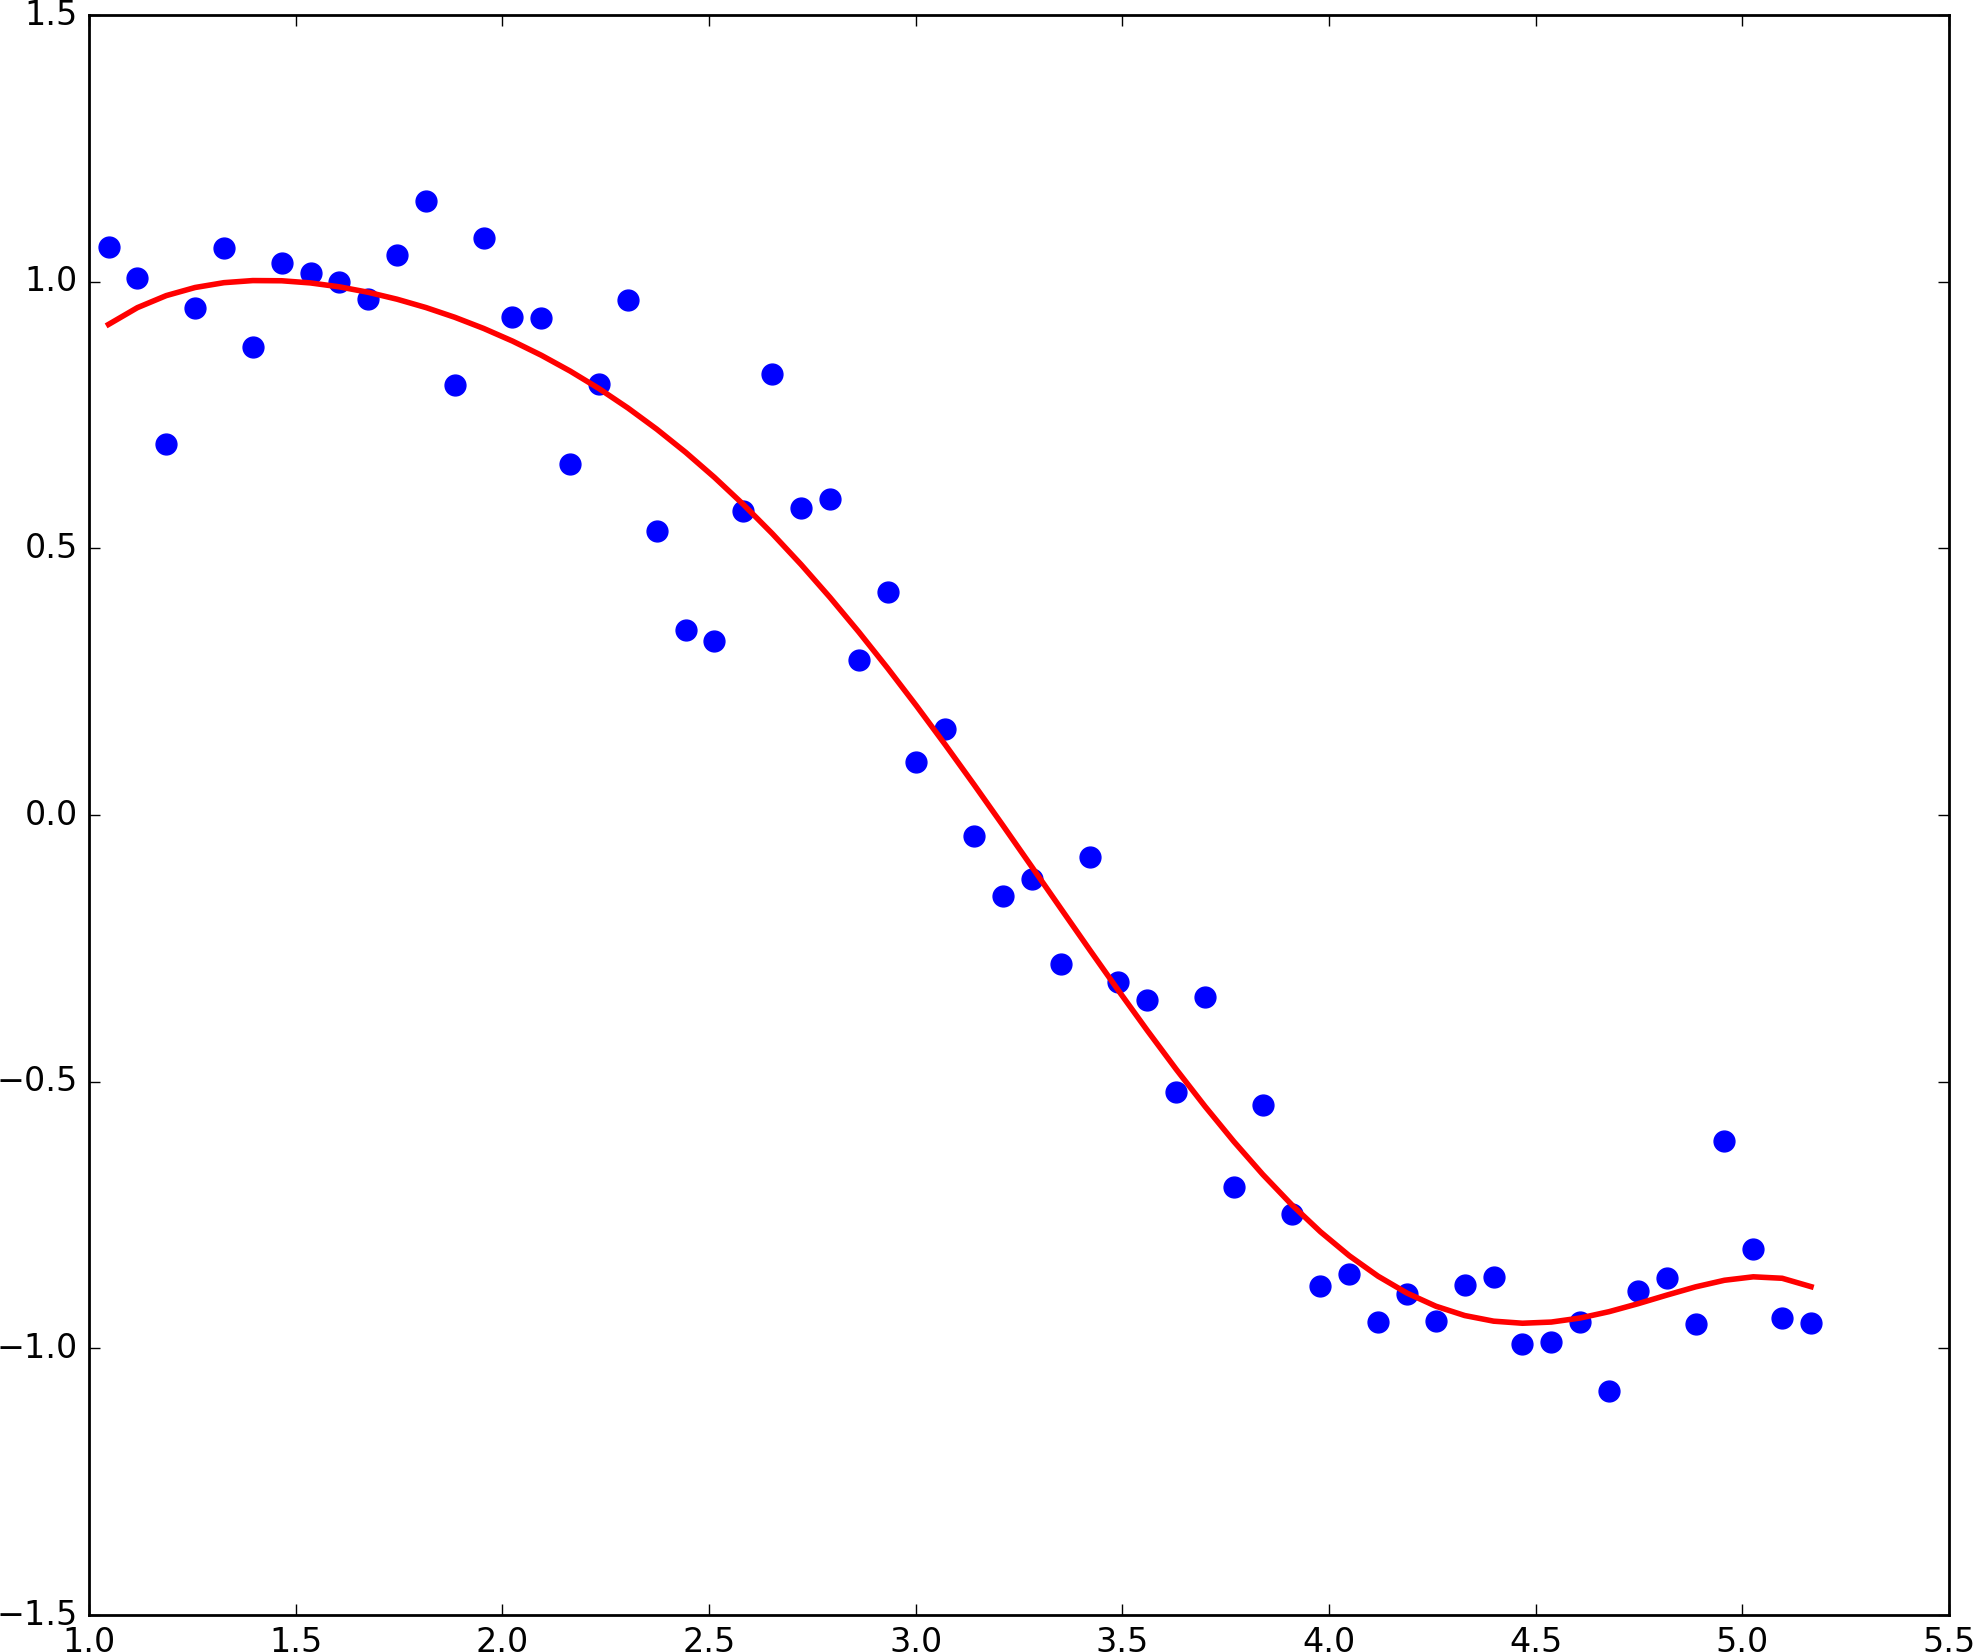
\includegraphics[width=0.99\textwidth]{./fig/linreg_pow4.png}
\end{figure}
\vspace{-2em}
\begin{figure}
$p=15$
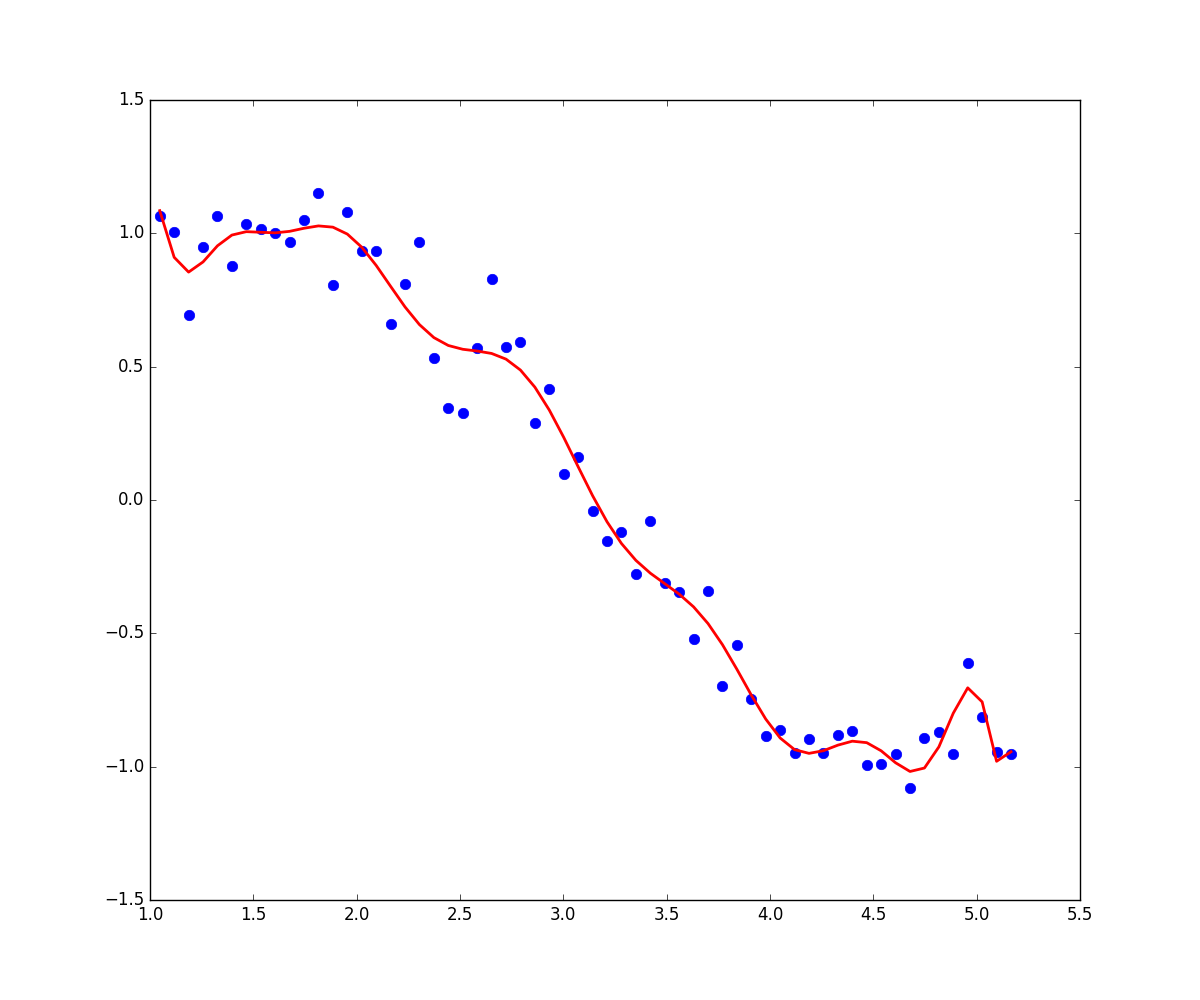
\includegraphics[width=0.99\textwidth]{./fig/linreg_pow15.png}
\end{figure}
\end{columns}
\end{frame}


%%%%%%%%%%%%%%%%%%%%%
\begin{frame}
\frametitle{Overfitting}
\begin{block}{}
When there is to many paramaters to fit, the model can reproduce 
a random noise, it is called \alert{overfitting}
\end{block}
\pause
\begin{table}
\resizebox{\textwidth}{!}{%
\begin{tabular}{lllllllllll}
\toprule
{} &      rmse &      th\_0 &      th\_1 &      th\_2 &      th\_3 &      th\_4 &      th\_5 &      th\_6 &      th\_7 &      th\_8 \\
\midrule
max\_pow\_1  & +5.47e-02 & +1.96e+00 & -6.20e-01 &       NaN &       NaN &       NaN &       NaN &       NaN &       NaN &       NaN \\
max\_pow\_2  & +5.46e-02 & +1.91e+00 & -5.83e-01 & -5.96e-03 &       NaN &       NaN &       NaN &       NaN &       NaN &       NaN \\
max\_pow\_3  & +1.84e-02 & -1.08e+00 & +3.03e+00 & -1.29e+00 & +1.37e-01 &       NaN &       NaN &       NaN &       NaN &       NaN \\
max\_pow\_4  & +1.80e-02 & -2.66e-01 & +1.69e+00 & -5.32e-01 & -3.57e-02 & +1.39e-02 &       NaN &       NaN &       NaN &       NaN \\
max\_pow\_5  & +1.70e-02 & +2.99e+00 & -5.12e+00 & +4.72e+00 & -1.93e+00 & +3.35e-01 & -2.07e-02 &       NaN &       NaN &       NaN \\
max\_pow\_6  & +1.65e-02 & -2.80e+00 & +9.52e+00 & -9.71e+00 & +5.23e+00 & -1.55e+00 & +2.33e-01 & -1.36e-02 &       NaN &       NaN \\
max\_pow\_7  & +1.55e-02 & +1.93e+01 & -5.60e+01 & +6.90e+01 & -4.46e+01 & +1.65e+01 & -3.53e+00 & +4.05e-01 & -1.92e-02 &       NaN \\
max\_pow\_8  & +1.53e-02 & +4.32e+01 & -1.37e+02 & +1.84e+02 & -1.33e+02 & +5.77e+01 & -1.53e+01 & +2.42e+00 & -2.10e-01 & +7.68e-03 \\
max\_pow\_9  & +1.46e-02 & +1.68e+02 & -6.15e+02 & +9.63e+02 & -8.46e+02 & +4.61e+02 & -1.62e+02 & +3.68e+01 & -5.22e+00 & +4.22e-01 \\
max\_pow\_10 & +1.46e-02 & +1.38e+02 & -4.86e+02 & +7.26e+02 & -5.96e+02 & +2.93e+02 & -8.75e+01 & +1.45e+01 & -8.06e-01 & -1.38e-01 \\
max\_pow\_11 & +1.45e-02 & -7.49e+01 & +5.12e+02 & -1.33e+03 & +1.87e+03 & -1.61e+03 & +9.14e+02 & -3.50e+02 & +9.14e+01 & -1.61e+01 \\
max\_pow\_12 & +1.45e-02 & -3.39e+02 & +1.87e+03 & -4.42e+03 & +6.01e+03 & -5.25e+03 & +3.12e+03 & -1.30e+03 & +3.84e+02 & -8.03e+01 \\
max\_pow\_13 & +1.43e-02 & +3.20e+03 & -1.78e+04 & +4.46e+04 & -6.66e+04 & +6.61e+04 & -4.61e+04 & +2.32e+04 & -8.55e+03 & +2.30e+03 \\
max\_pow\_14 & +1.31e-02 & +2.38e+04 & -1.41e+05 & +3.79e+05 & -6.10e+05 & +6.57e+05 & -5.03e+05 & +2.82e+05 & -1.17e+05 & +3.66e+04 \\
max\_pow\_15 & +1.17e-02 & -3.62e+04 & +2.44e+05 & -7.46e+05 & +1.38e+06 & -1.71e+06 & +1.53e+06 & -1.00e+06 & +4.98e+05 & -1.88e+05 \\
\bottomrule
\end{tabular}
}
\end{table}
\end{frame}


%%%%%%%%%%%%%%%%%%%%%%%
\begin{frame}
\frametitle{High parameters values}
\begin{figure}
Value of the parameters $|\theta_1|$ with respect with the degree of the polynomial
regression\\
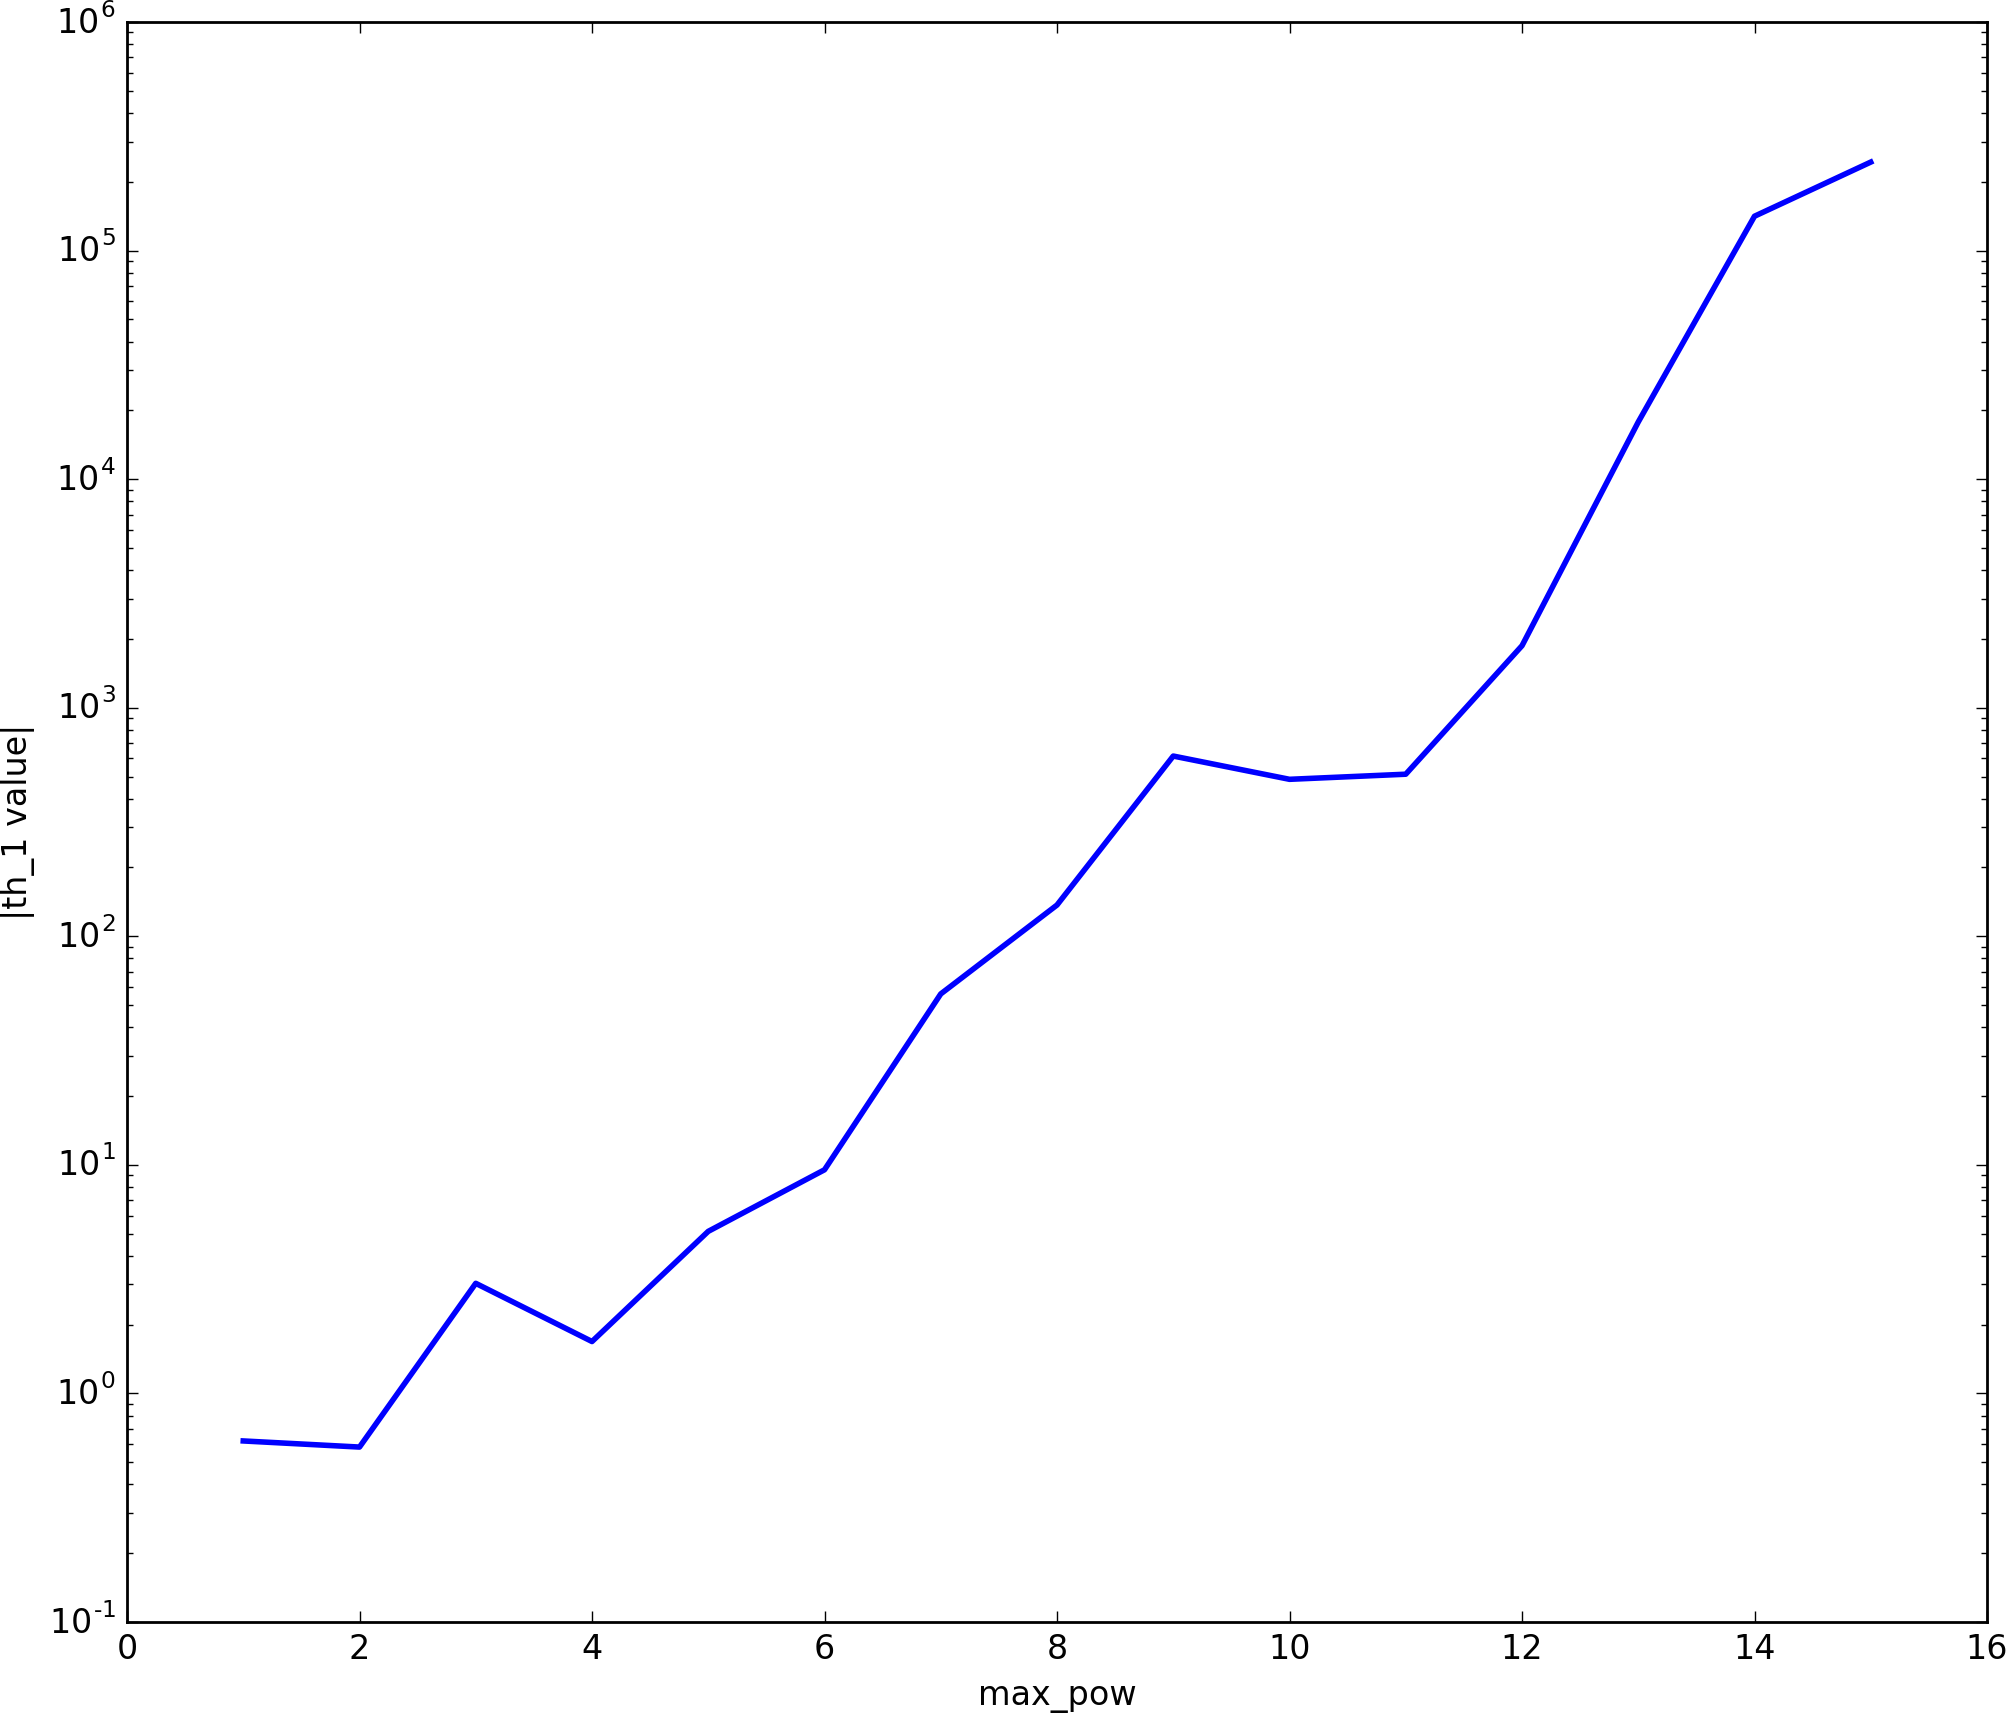
\includegraphics[height=0.75\textheight]{./fig/coefs_th1.png}
\end{figure}

\end{frame}

%%%%%%%%%%%%%%%%%%%%%
\begin{frame}
\frametitle{Regularization}
\begin{block}{The idea}
The idea of regularization is to perform a regression minimizing a cost function
that includes a term to penalize "big" values for the parameters:
$$
J(\bm{\theta}) = \frac{1}{n} \sum (y_i - h_{\bm{\theta}}(x_i))^2 + \alpha P(\bm{\theta})
$$
\end{block}
\pause
We consider two penality terms:
\begin{itemize}[<+->]
\item \alert{Ridge Regularization:} $P(\bm{\theta}) = \sum_{i=0}^p \theta_i^2$
\item \alert{Lasso Regularization:} $P(\bm{\theta}) = \sum_{i=0}^p |\theta_i|$
\item Elastic Net combines both regulariztion
\end{itemize}

\end{frame}

%%%%%%%%%%%%%%%%%%%%
\begin{frame}
\frametitle{Ridge regression}
\begin{block}{}
Ridge regression is a linear regression with a Ridge regularization:
$$
J(\bm{\theta}) = \frac{1}{n} \sum (y_i - h_{\bm{\theta}}(x_i))^2 + \alpha \sum_{i=0}^p \theta_i^2
$$
\end{block}
\end{frame}

%%%%%%%%%%%%%%%%%%%%
\begin{frame}
\frametitle{Results for $p=15$ and varying $\alpha$}
\begin{columns}
\column{.33\textwidth}
\vspace{-2em}
\begin{figure}
$\alpha=0$
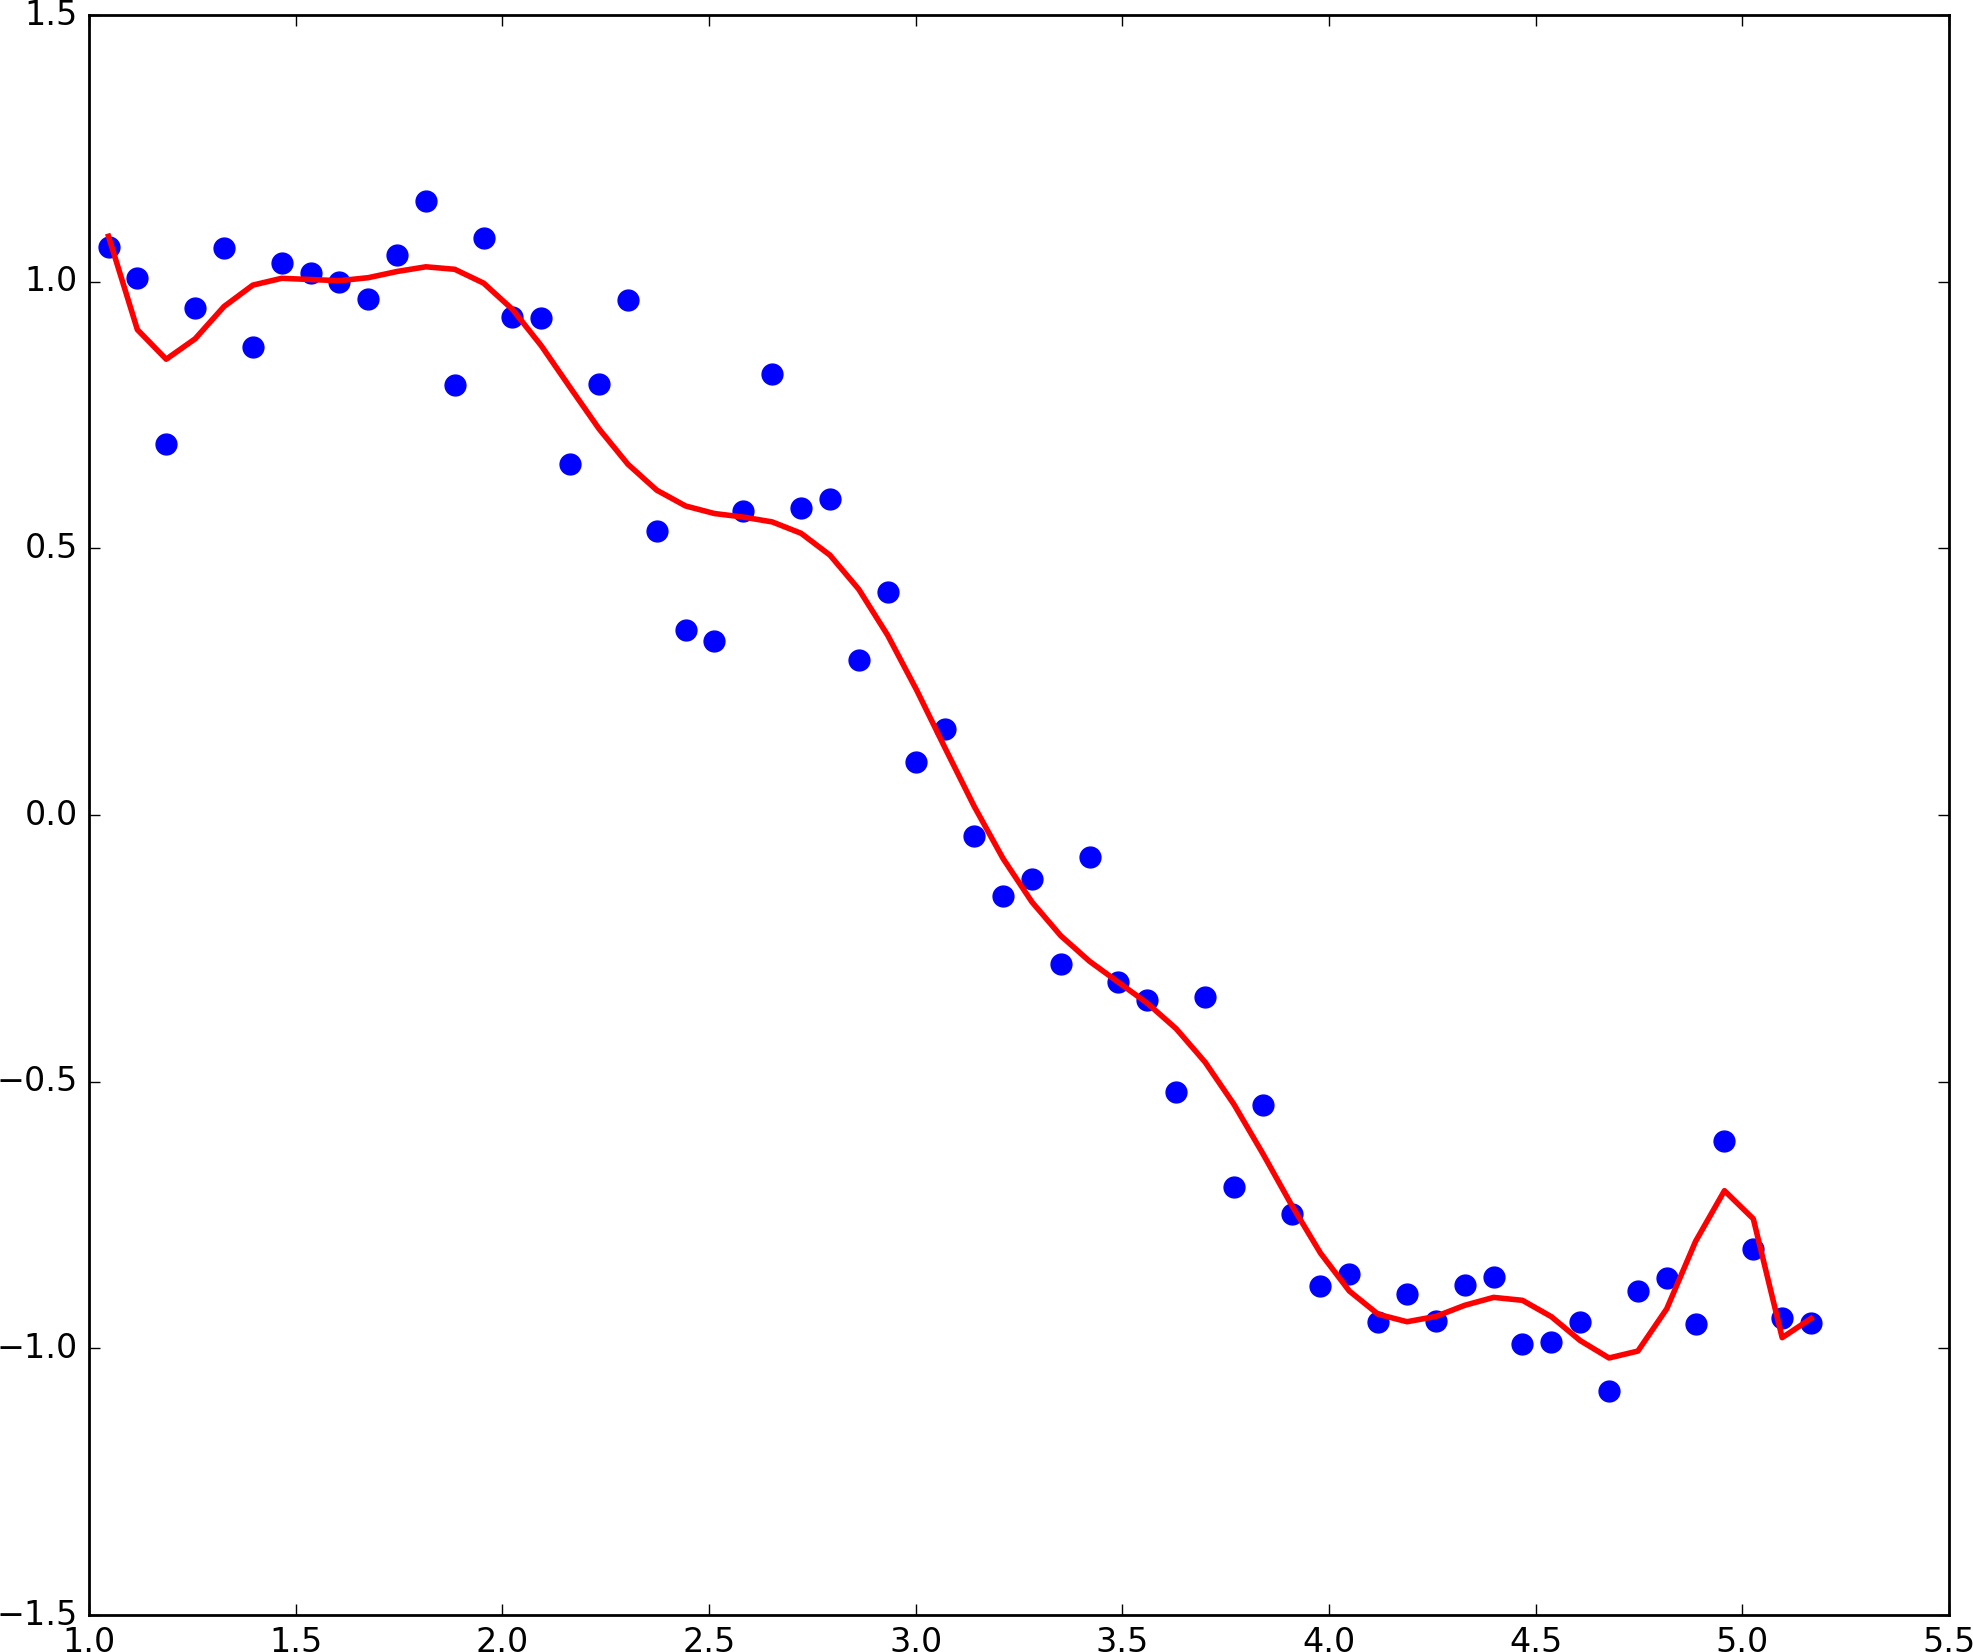
\includegraphics[width=0.99\textwidth]{./fig/ridge_alpha0.png}
\end{figure}
\vspace{-2em}
\begin{figure}
$\alpha=1e-3$
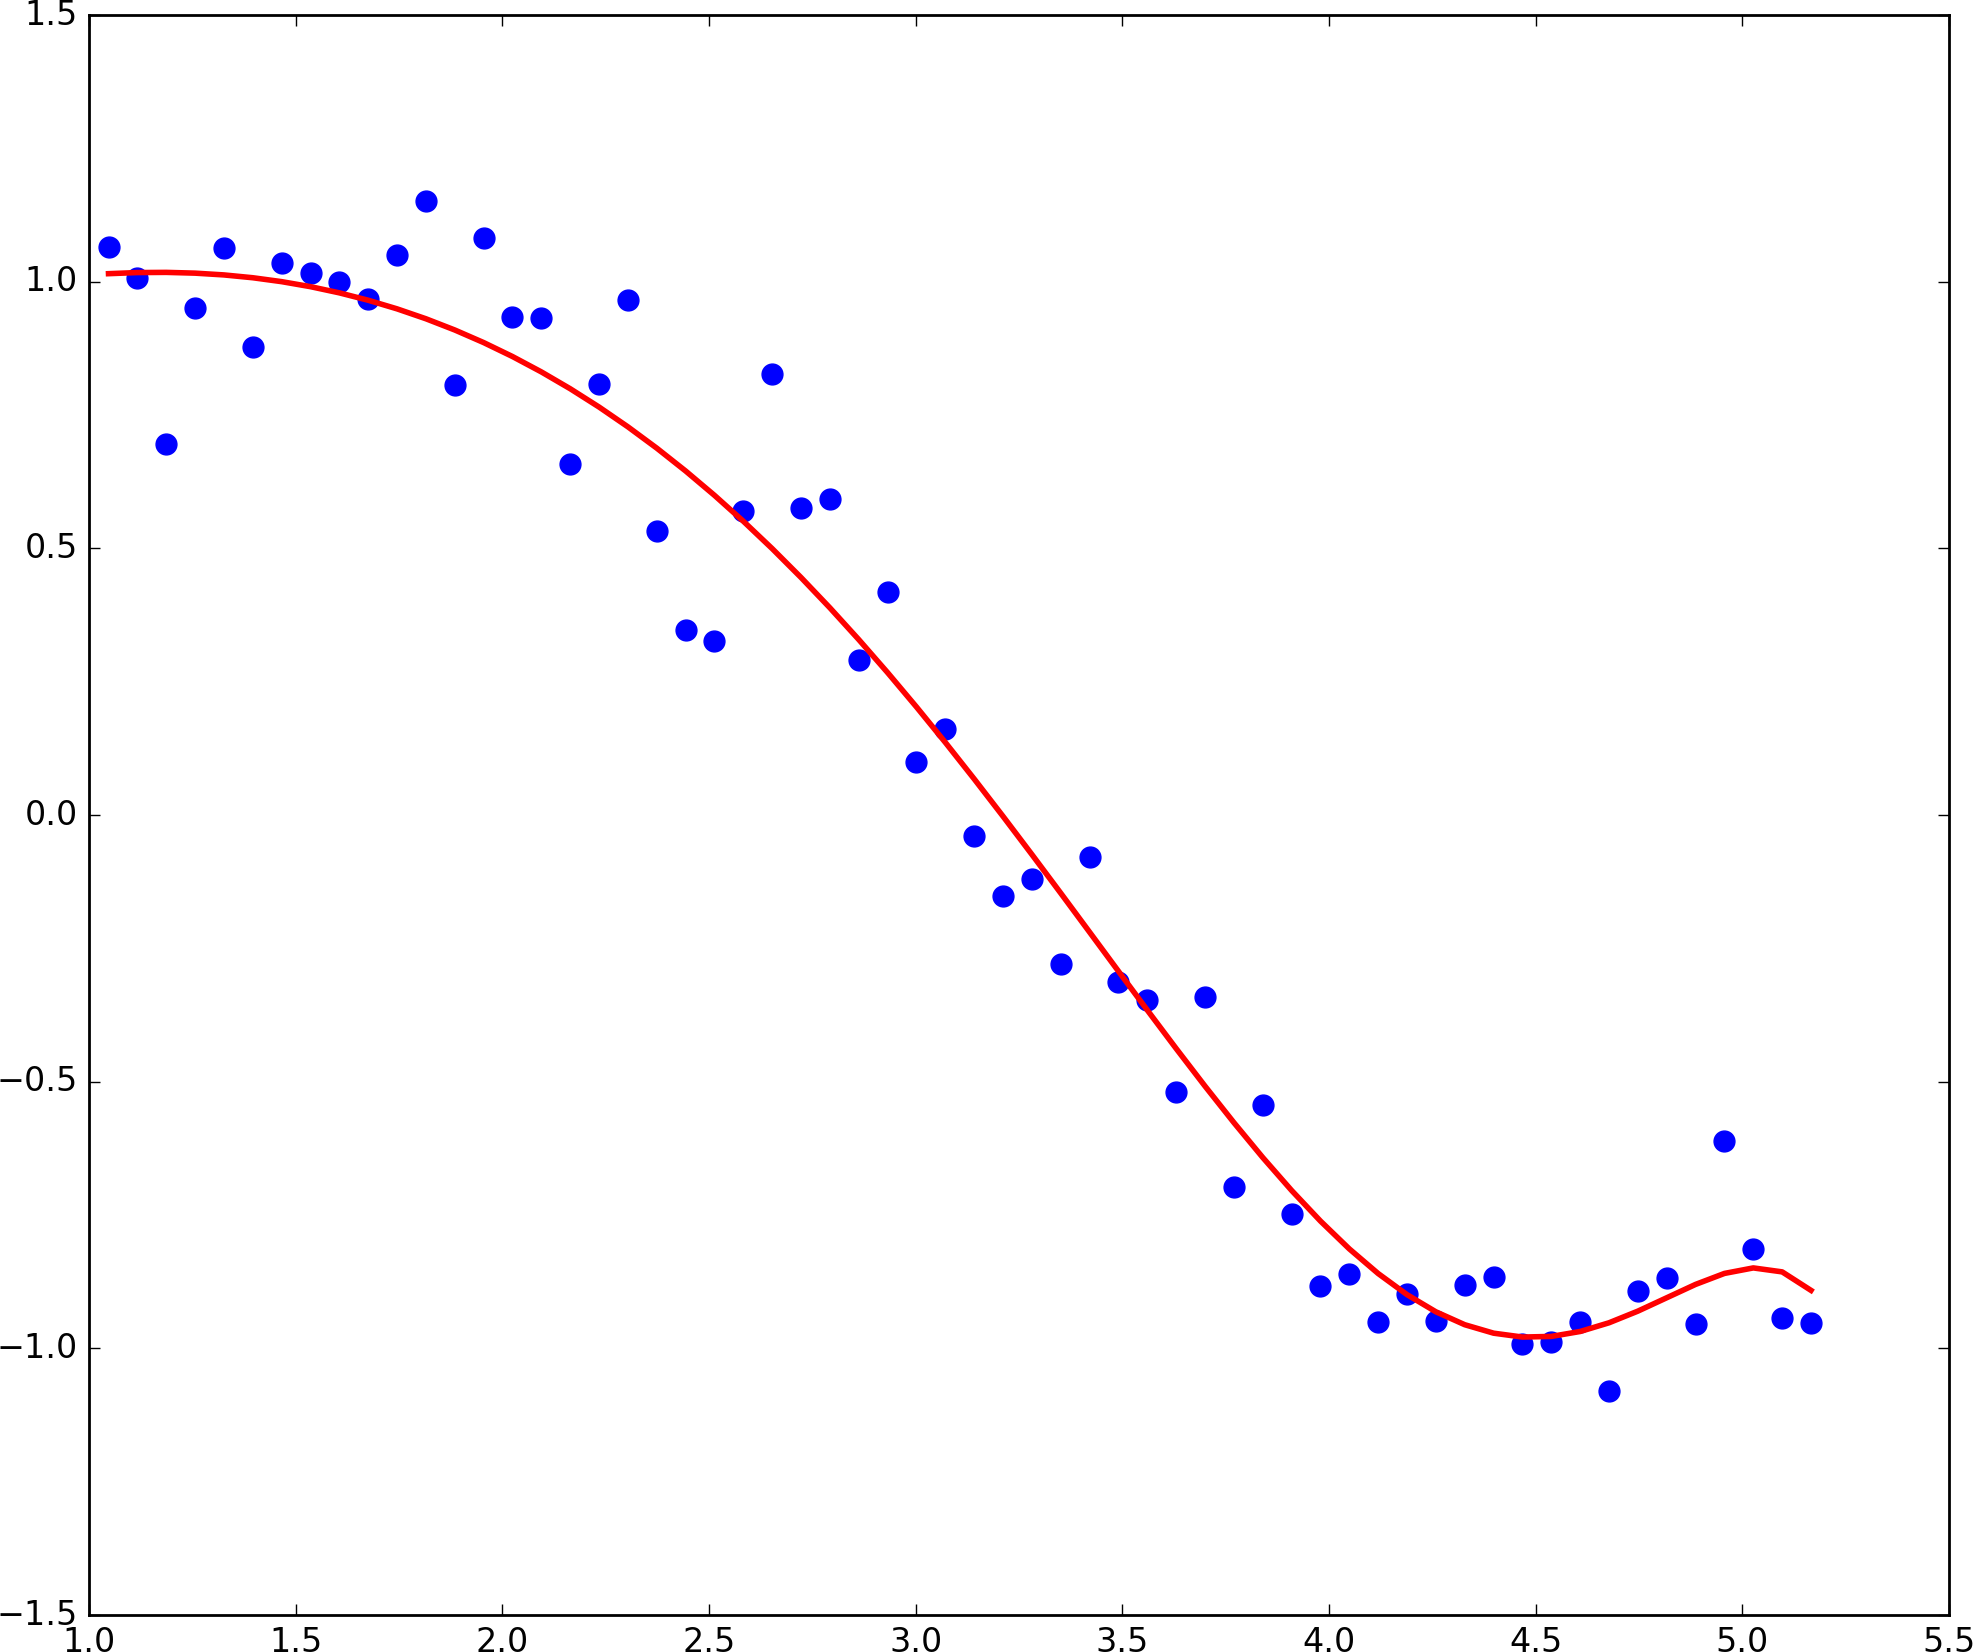
\includegraphics[width=0.99\textwidth]{./fig/ridge_alpha1e-3.png}
\end{figure}
\column{.33\textwidth}
\vspace{-2em}
\begin{figure}
$\alpha=1e-15$
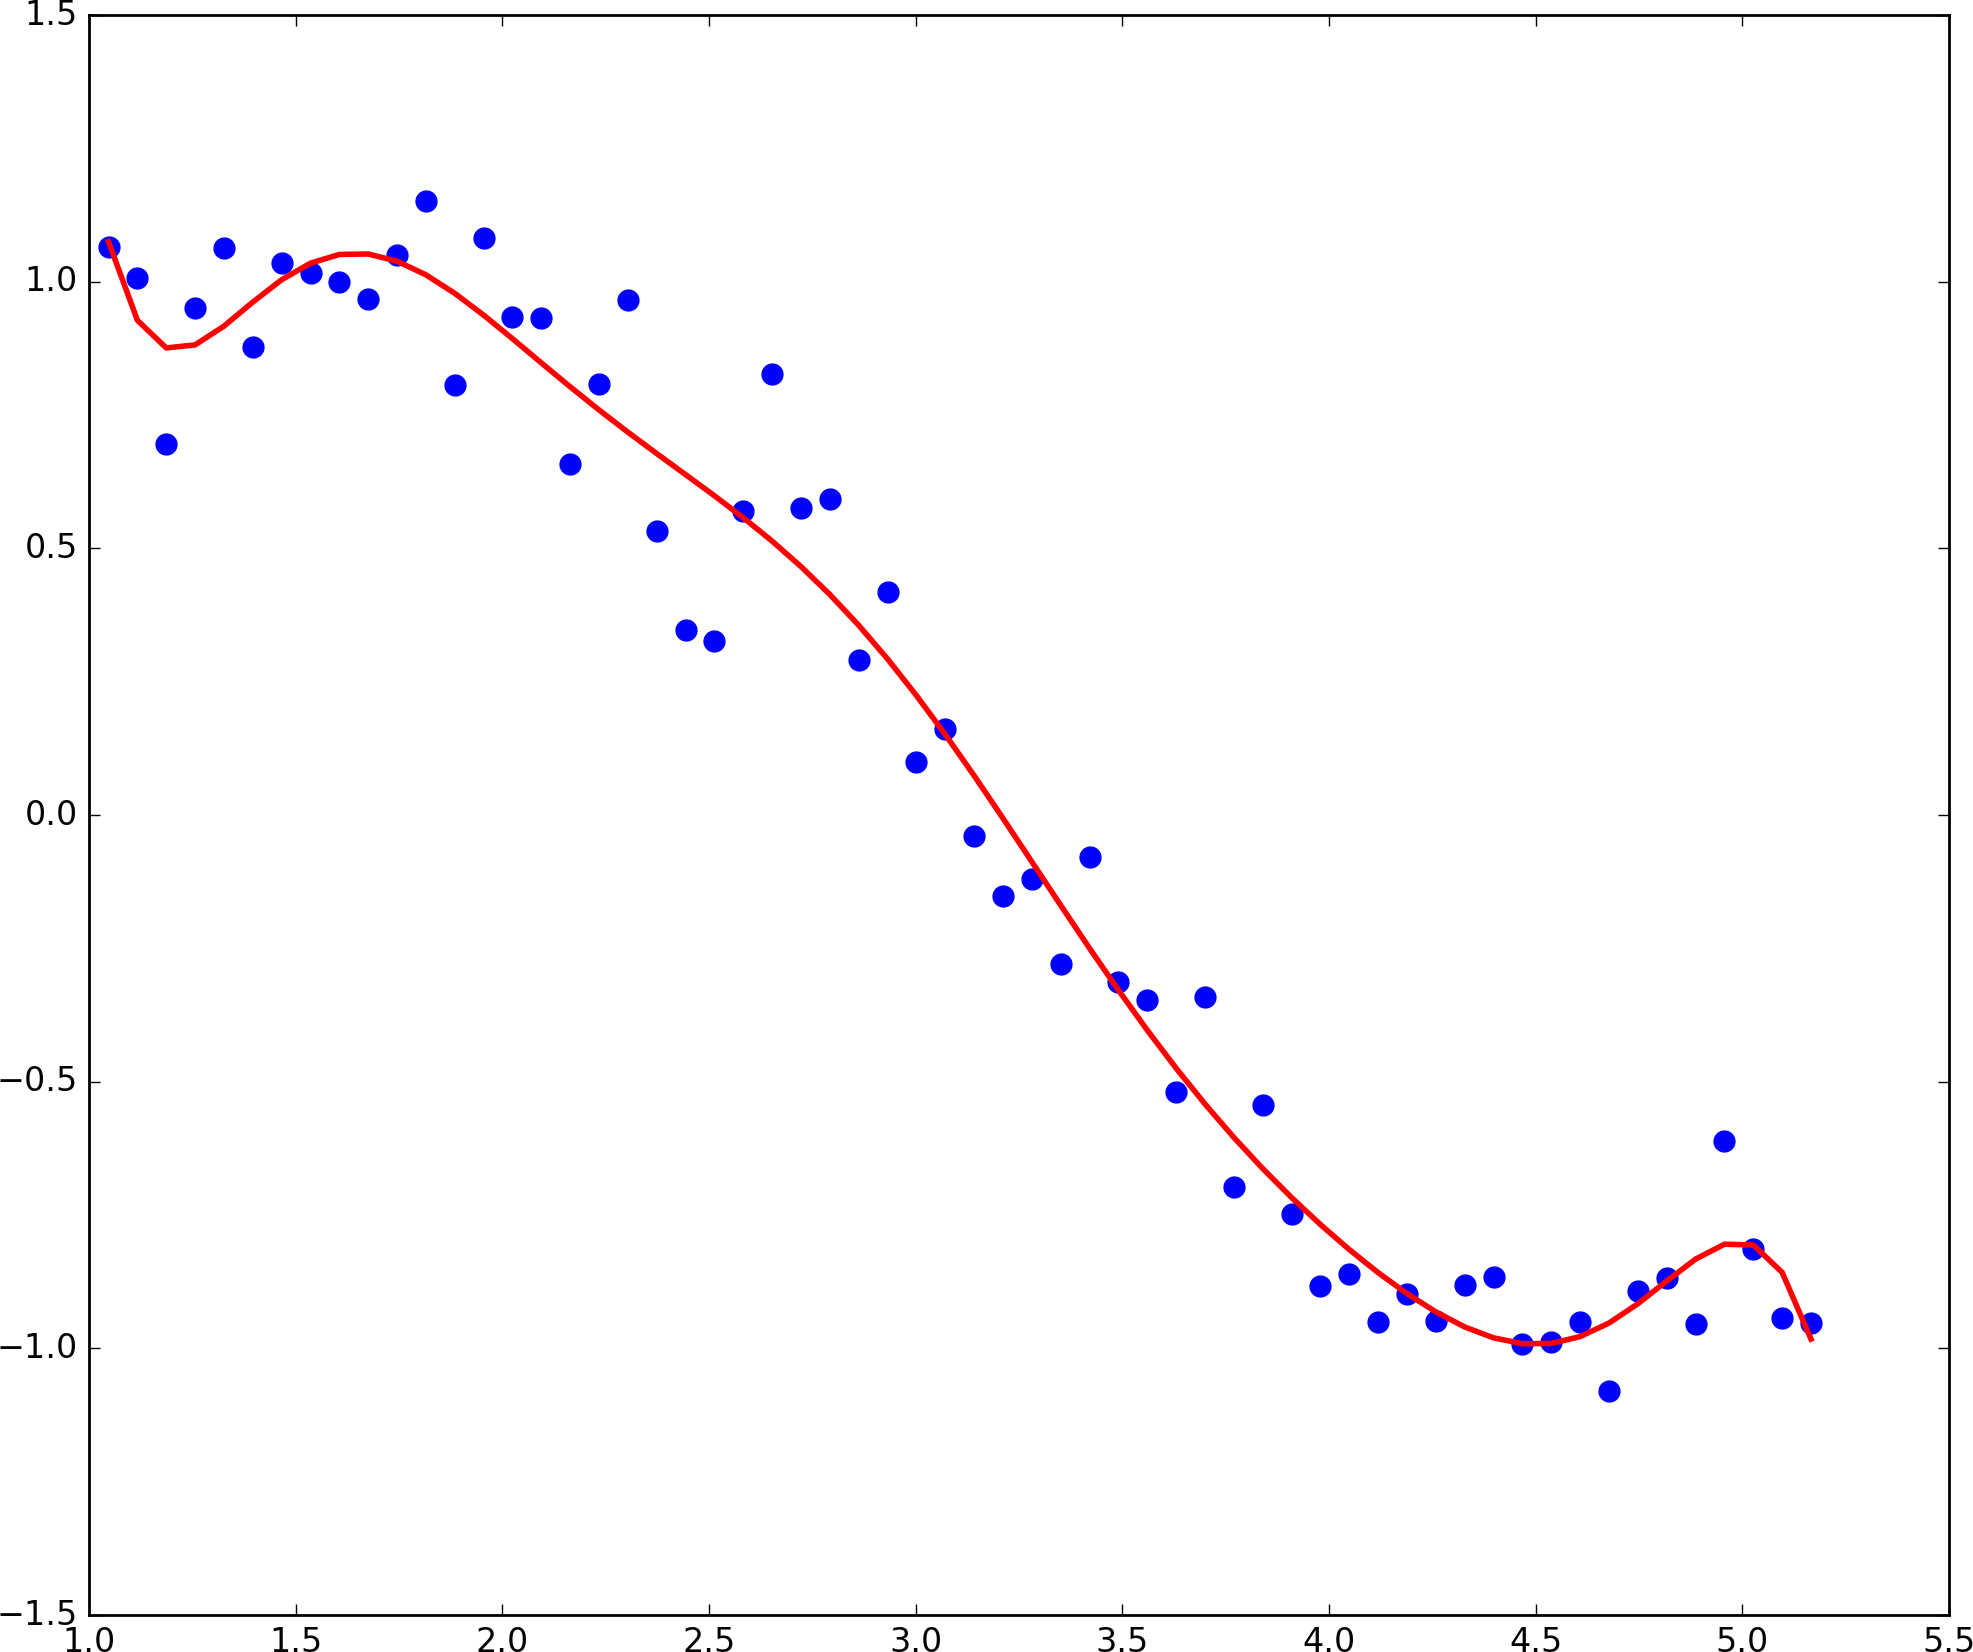
\includegraphics[width=0.99\textwidth]{./fig/ridge_alpha1e-15.png}
\end{figure}
\vspace{-2em}
\begin{figure}
$\alpha=1e-2$
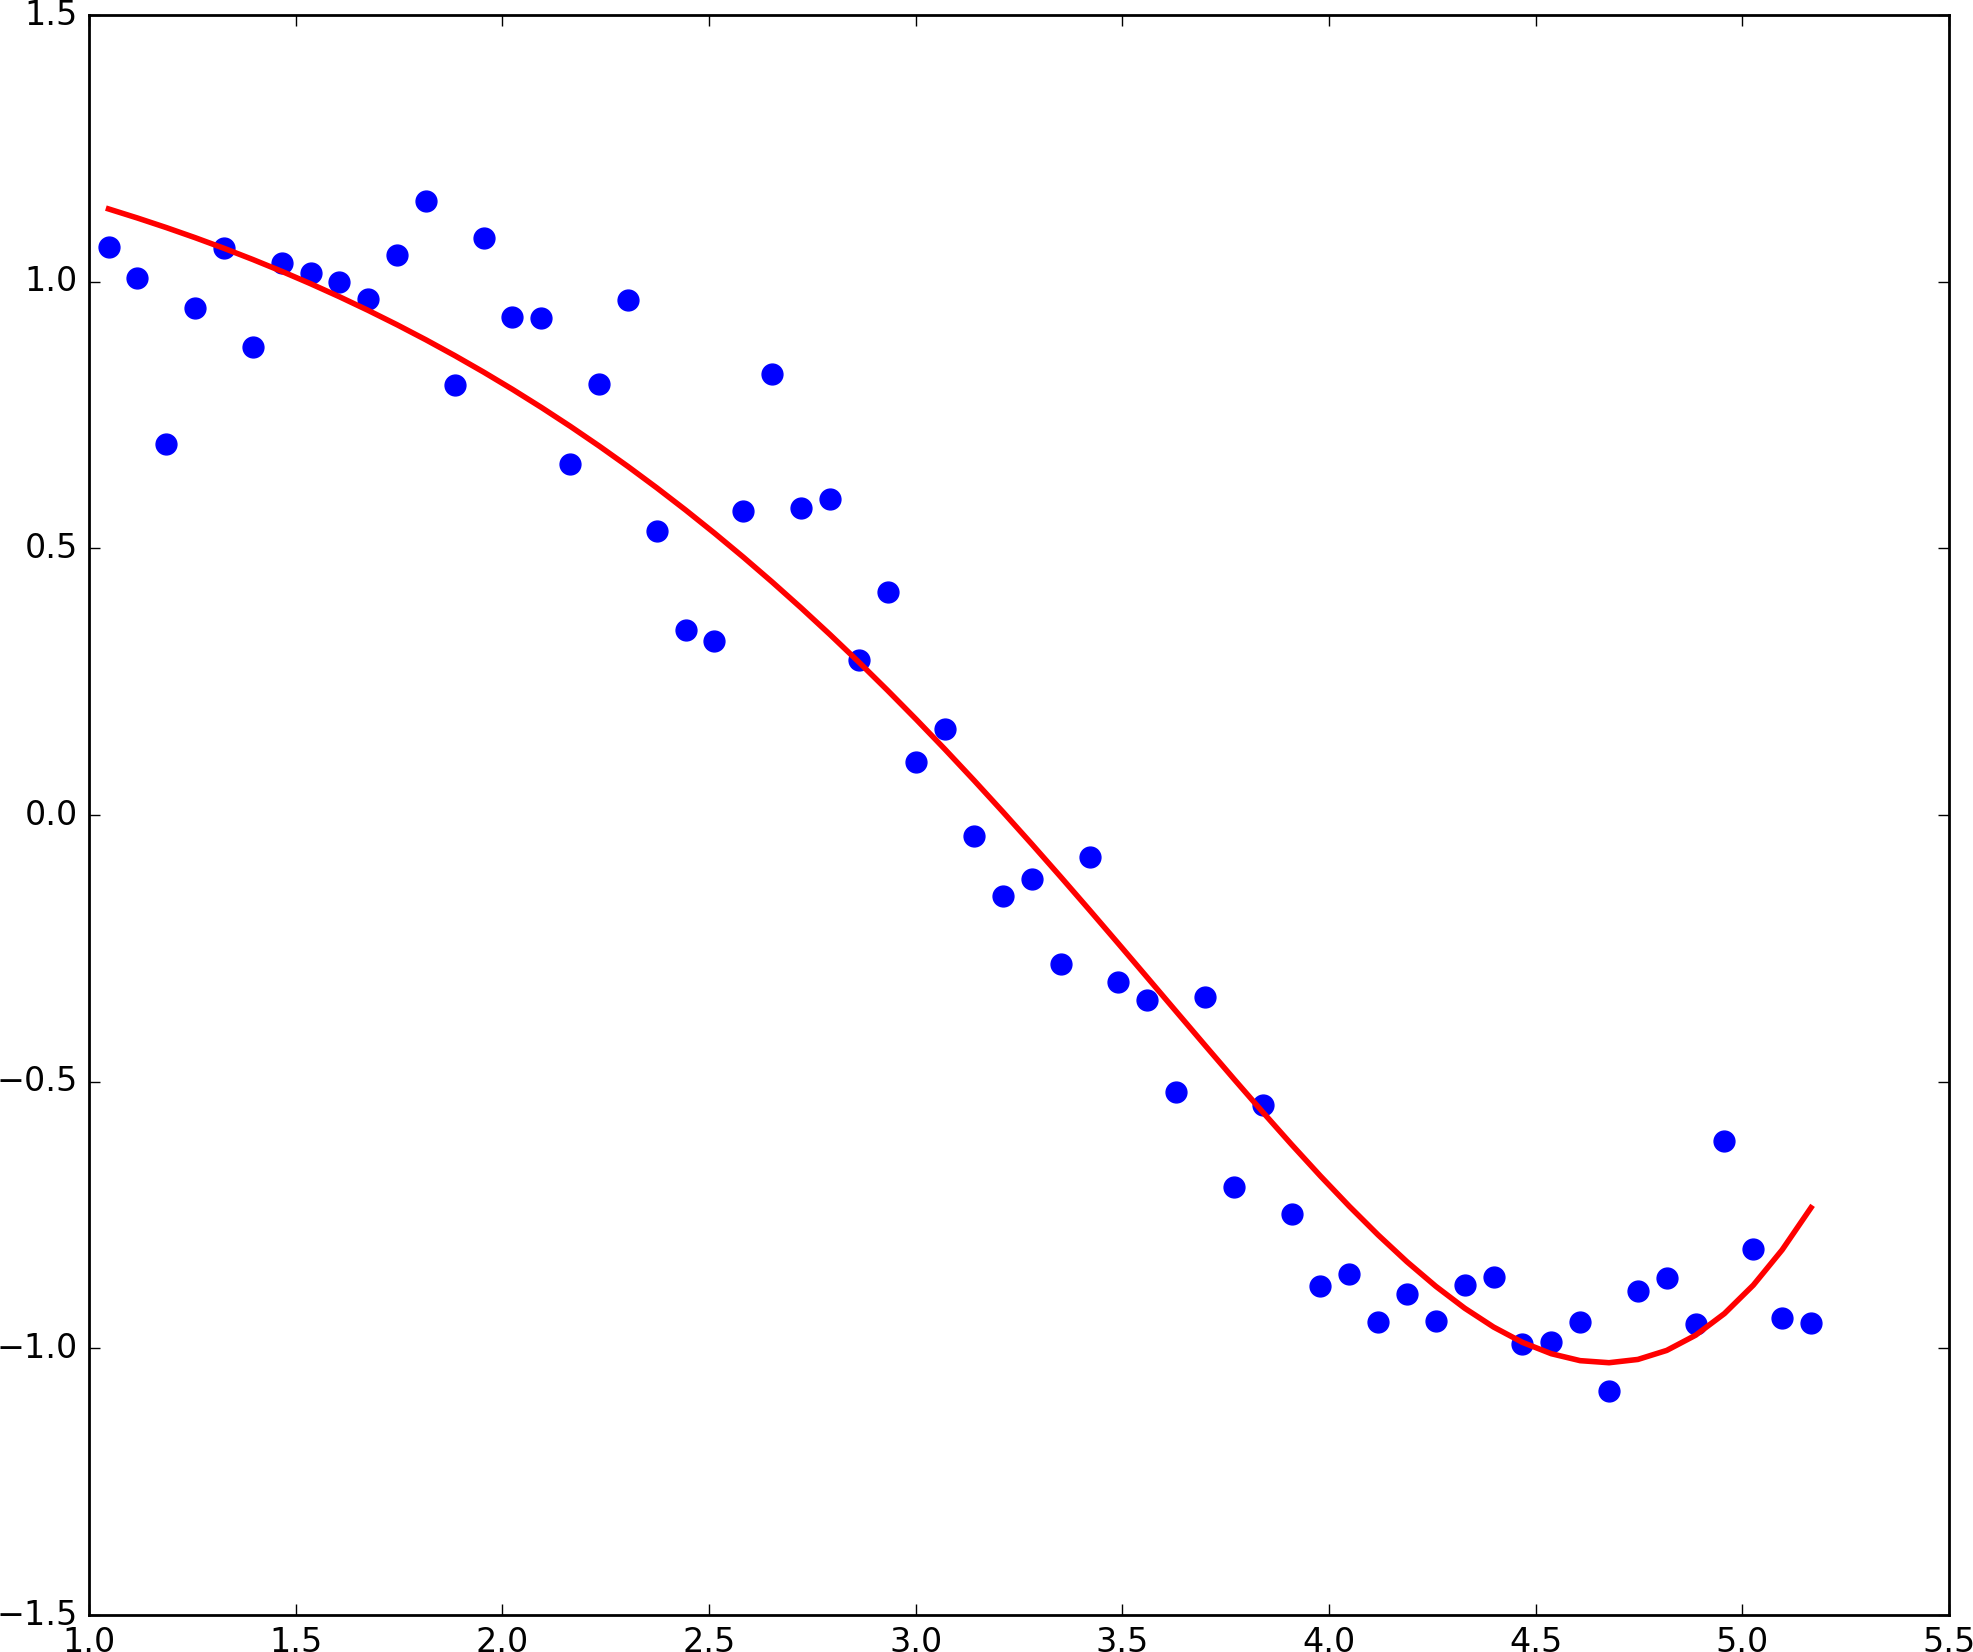
\includegraphics[width=0.99\textwidth]{./fig/ridge_alpha1e-2.png}
\end{figure}
\column{.33\textwidth}
\vspace{-2em}
\begin{figure}
$\alpha=1e-4$
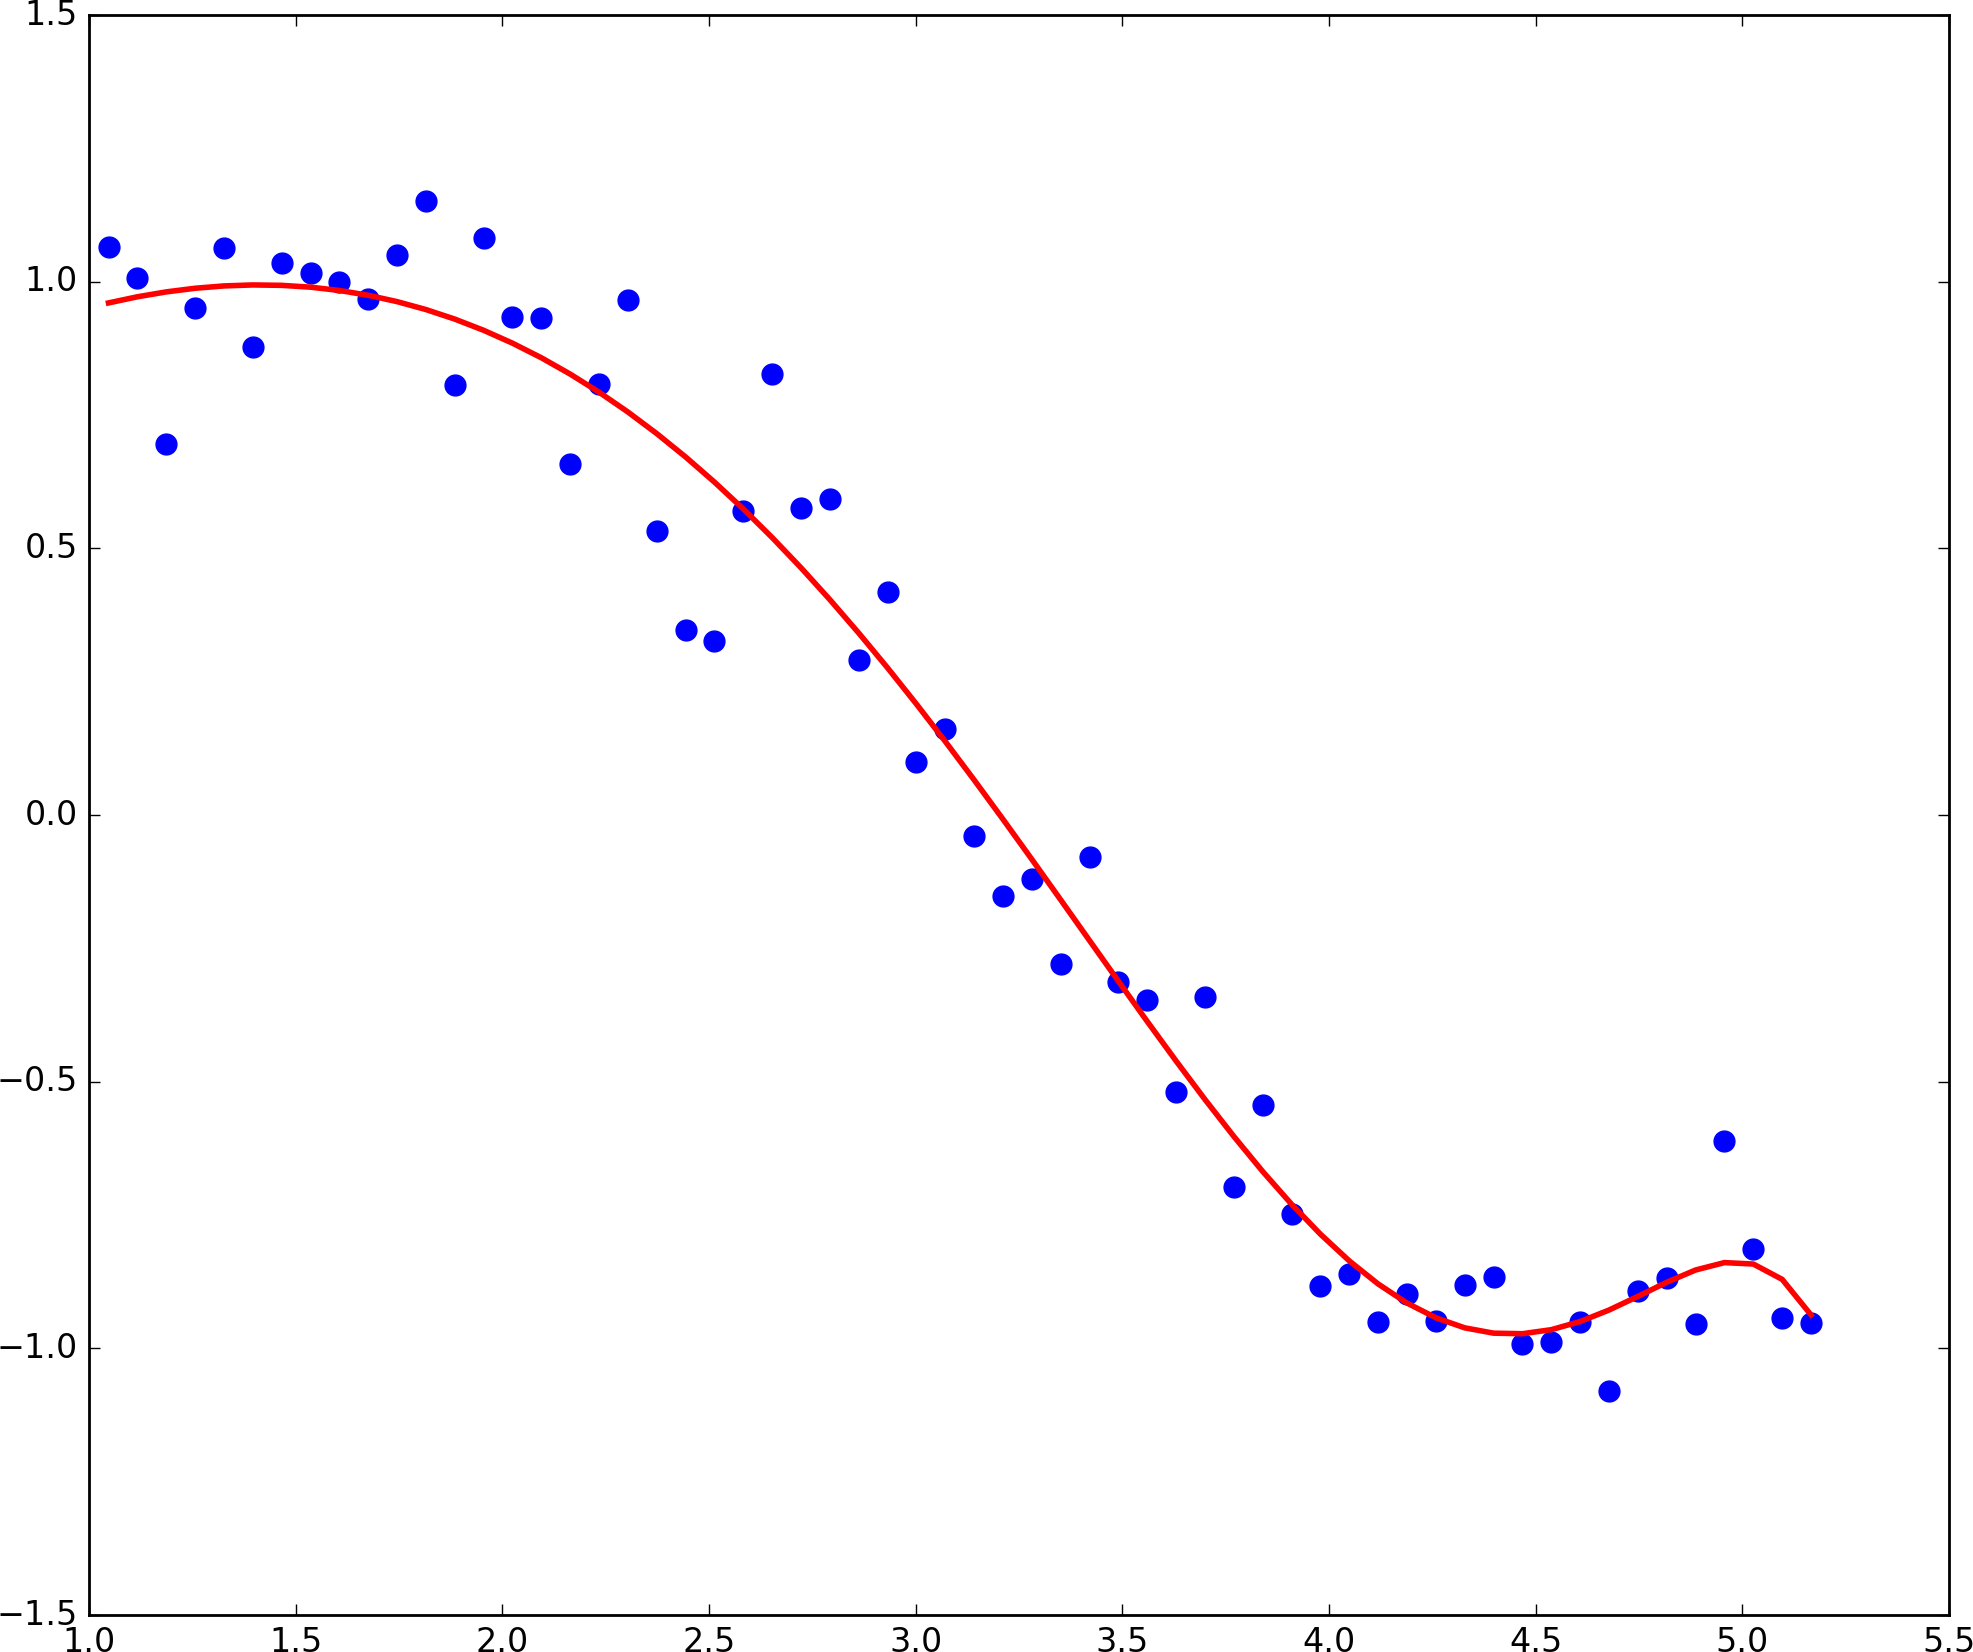
\includegraphics[width=0.99\textwidth]{./fig/ridge_alpha1e-4.png}
\end{figure}
\vspace{-2em}
\begin{figure}
$\alpha=5$
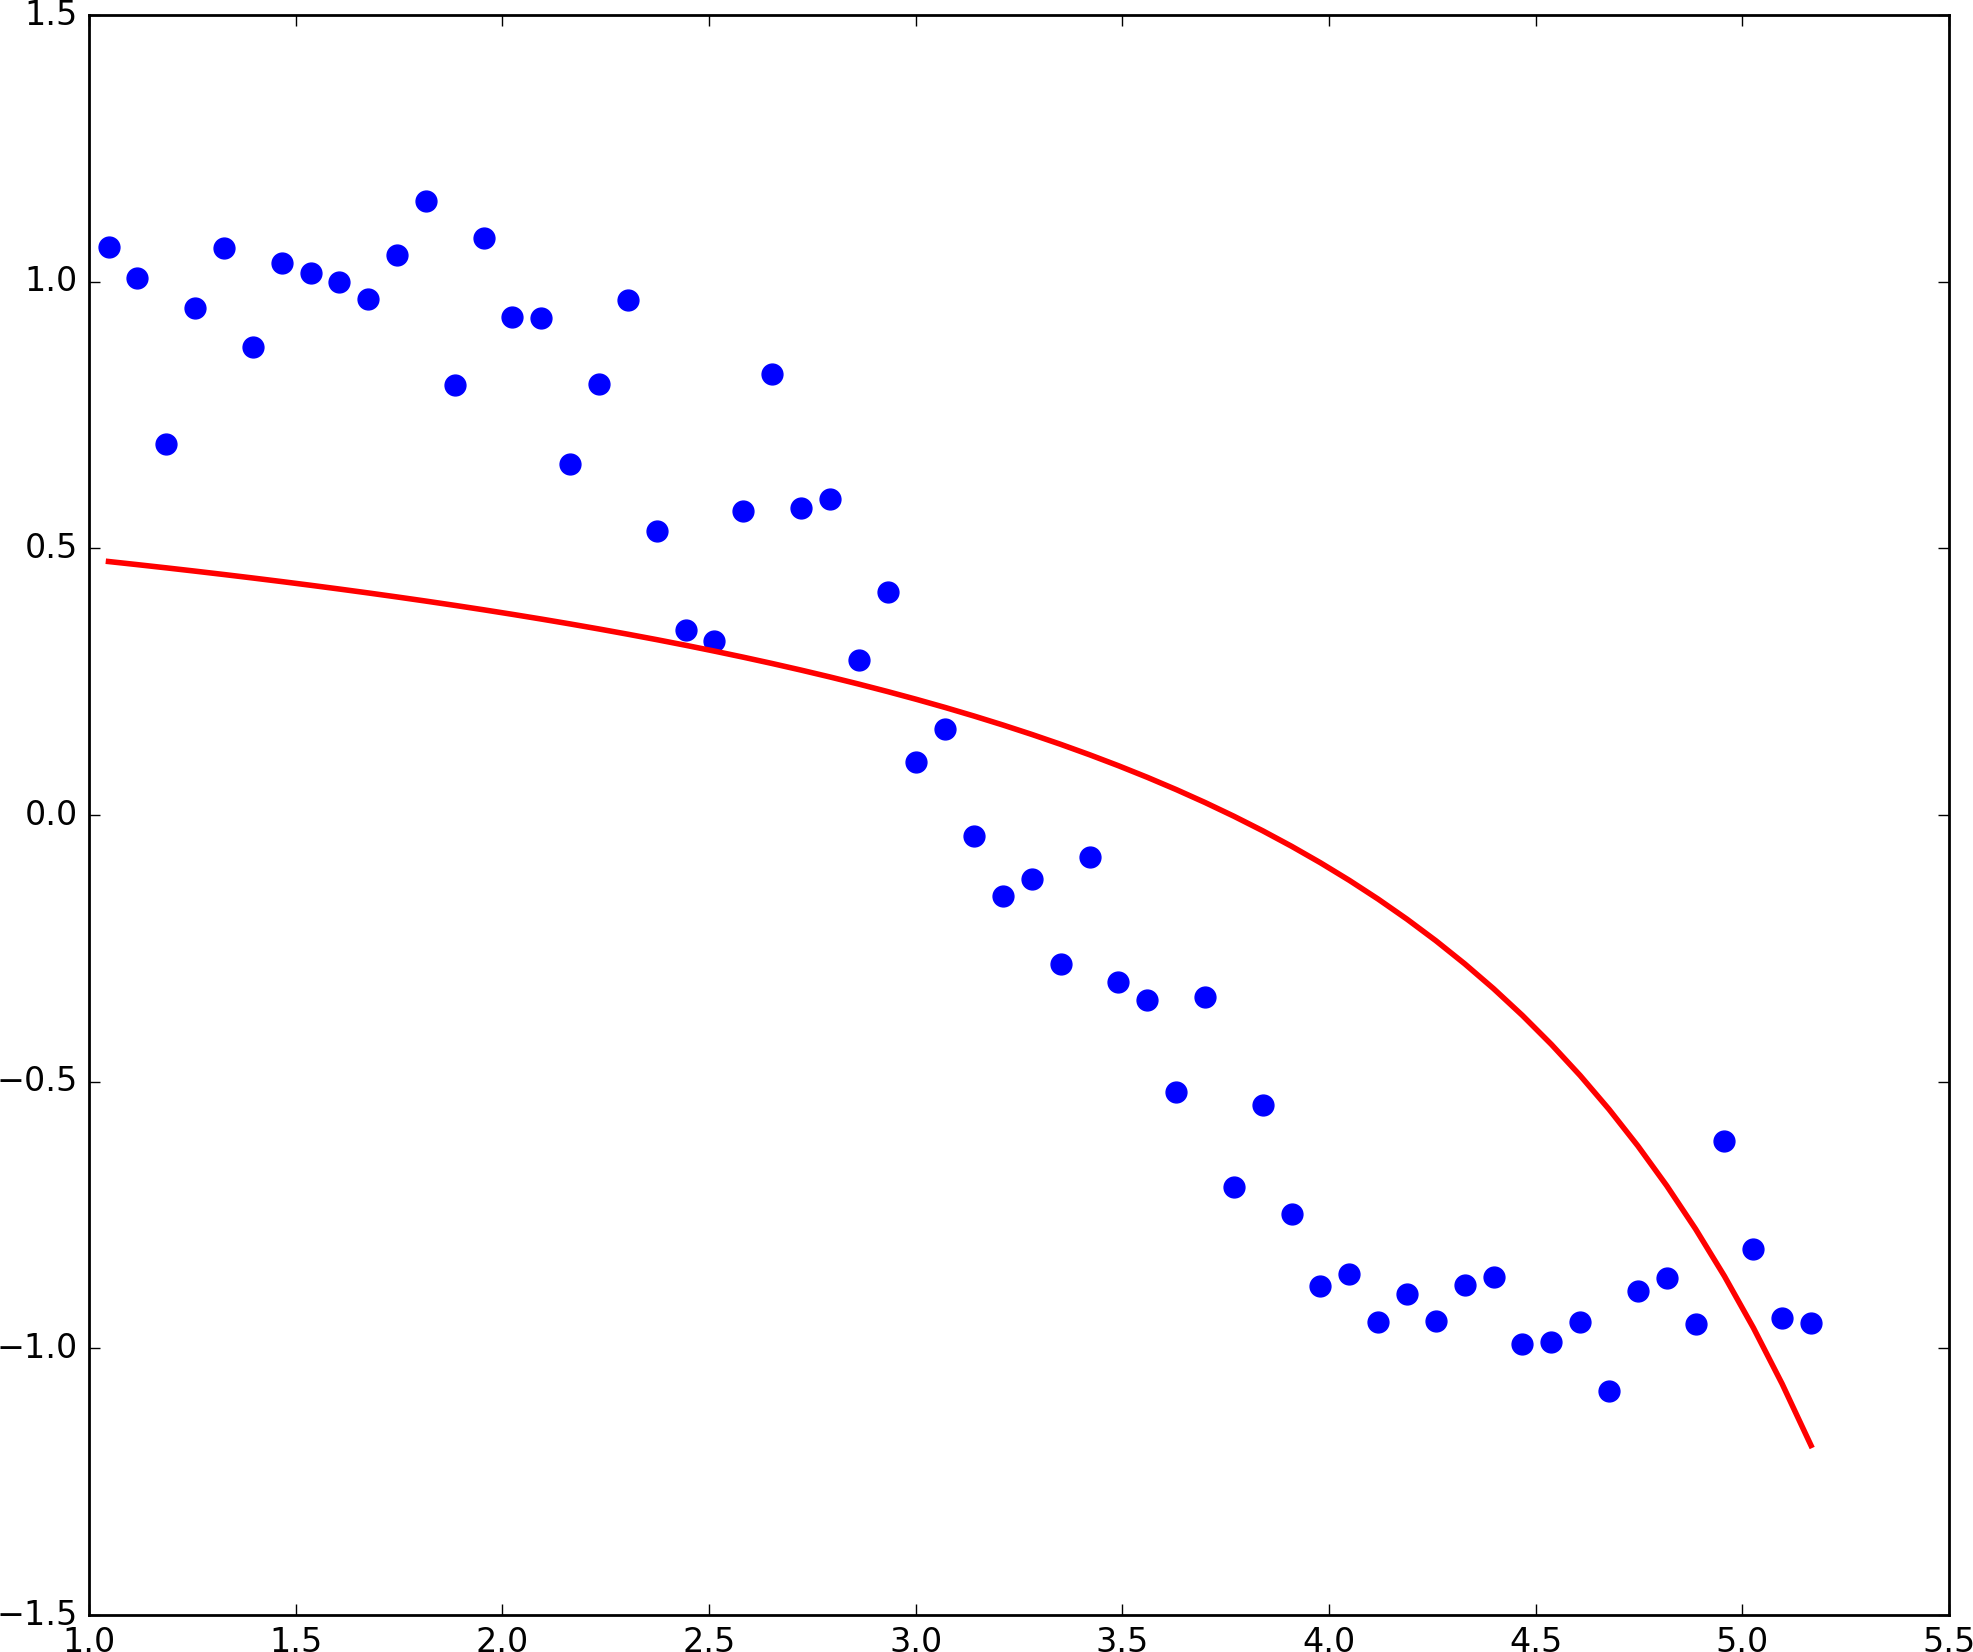
\includegraphics[width=0.99\textwidth]{./fig/ridge_alpha5.png}
\end{figure}
\end{columns}
\end{frame}

%%%%%%%%%%%%%%%%%%%%%
\begin{frame}
\frametitle{Values of coefficients}
\vspace{-2em}
\begin{table}
\resizebox{\textwidth}{!}{%
\begin{tabular}{lllllllllll}
\toprule
{} &      rmse &      th\_0 &      th\_1 &      th\_2 &      th\_3 &      th\_4 &      th\_5 &      th\_6 &      th\_7 &      th\_8 \\
\midrule
alpha\_0      & +7.05e-01 & -3.62e+04 & +2.44e+05 & -7.46e+05 & +1.38e+06 & -1.71e+06 & +1.53e+06 & -1.00e+06 & +4.98e+05 & -1.88e+05 \\
alpha\_1e-15  & +9.57e-01 & +2.22e-01 & +1.06e+00 & -3.69e-01 & +8.85e-04 & +1.63e-03 & -1.19e-04 & -6.44e-05 & -6.28e-06 & +1.45e-06 \\
alpha\_1e-10  & +9.57e-01 & +2.22e-01 & +1.06e+00 & -3.69e-01 & +8.84e-04 & +1.63e-03 & -1.18e-04 & -6.44e-05 & -6.28e-06 & +1.45e-06 \\
alpha\_1e-08  & +9.57e-01 & +2.22e-01 & +1.06e+00 & -3.69e-01 & +7.69e-04 & +1.62e-03 & -1.10e-04 & -6.45e-05 & -6.32e-06 & +1.43e-06 \\
alpha\_0.0001 & +1.03e+00 & +9.03e-01 & +1.71e-01 & -0.00e+00 & -4.78e-02 & -0.00e+00 & -0.00e+00 & +0.00e+00 & +0.00e+00 & +9.47e-06 \\
alpha\_0.001  & +1.68e+00 & +1.29e+00 & -0.00e+00 & -1.26e-01 & -0.00e+00 & -0.00e+00 & -0.00e+00 & +0.00e+00 & +0.00e+00 & +0.00e+00 \\
alpha\_0.01   & +3.64e+00 & +1.76e+00 & -5.52e-01 & -5.62e-04 & -0.00e+00 & -0.00e+00 & -0.00e+00 & -0.00e+00 & -0.00e+00 & -0.00e+00 \\
alpha\_1      & +3.69e+01 & +3.80e-02 & -0.00e+00 & -0.00e+00 & -0.00e+00 & -0.00e+00 & -0.00e+00 & -0.00e+00 & -0.00e+00 & -0.00e+00 \\
alpha\_5      & +3.69e+01 & +3.80e-02 & -0.00e+00 & -0.00e+00 & -0.00e+00 & -0.00e+00 & -0.00e+00 & -0.00e+00 & -0.00e+00 & -0.00e+00 \\
alpha\_10     & +3.69e+01 & +3.80e-02 & -0.00e+00 & -0.00e+00 & -0.00e+00 & -0.00e+00 & -0.00e+00 & -0.00e+00 & -0.00e+00 & -0.00e+00 \\
alpha\_20     & +3.69e+01 & +3.80e-02 & -0.00e+00 & -0.00e+00 & -0.00e+00 & -0.00e+00 & -0.00e+00 & -0.00e+00 & -0.00e+00 & -0.00e+00 \\
\bottomrule
\end{tabular}
}
\end{table}
\begin{figure}
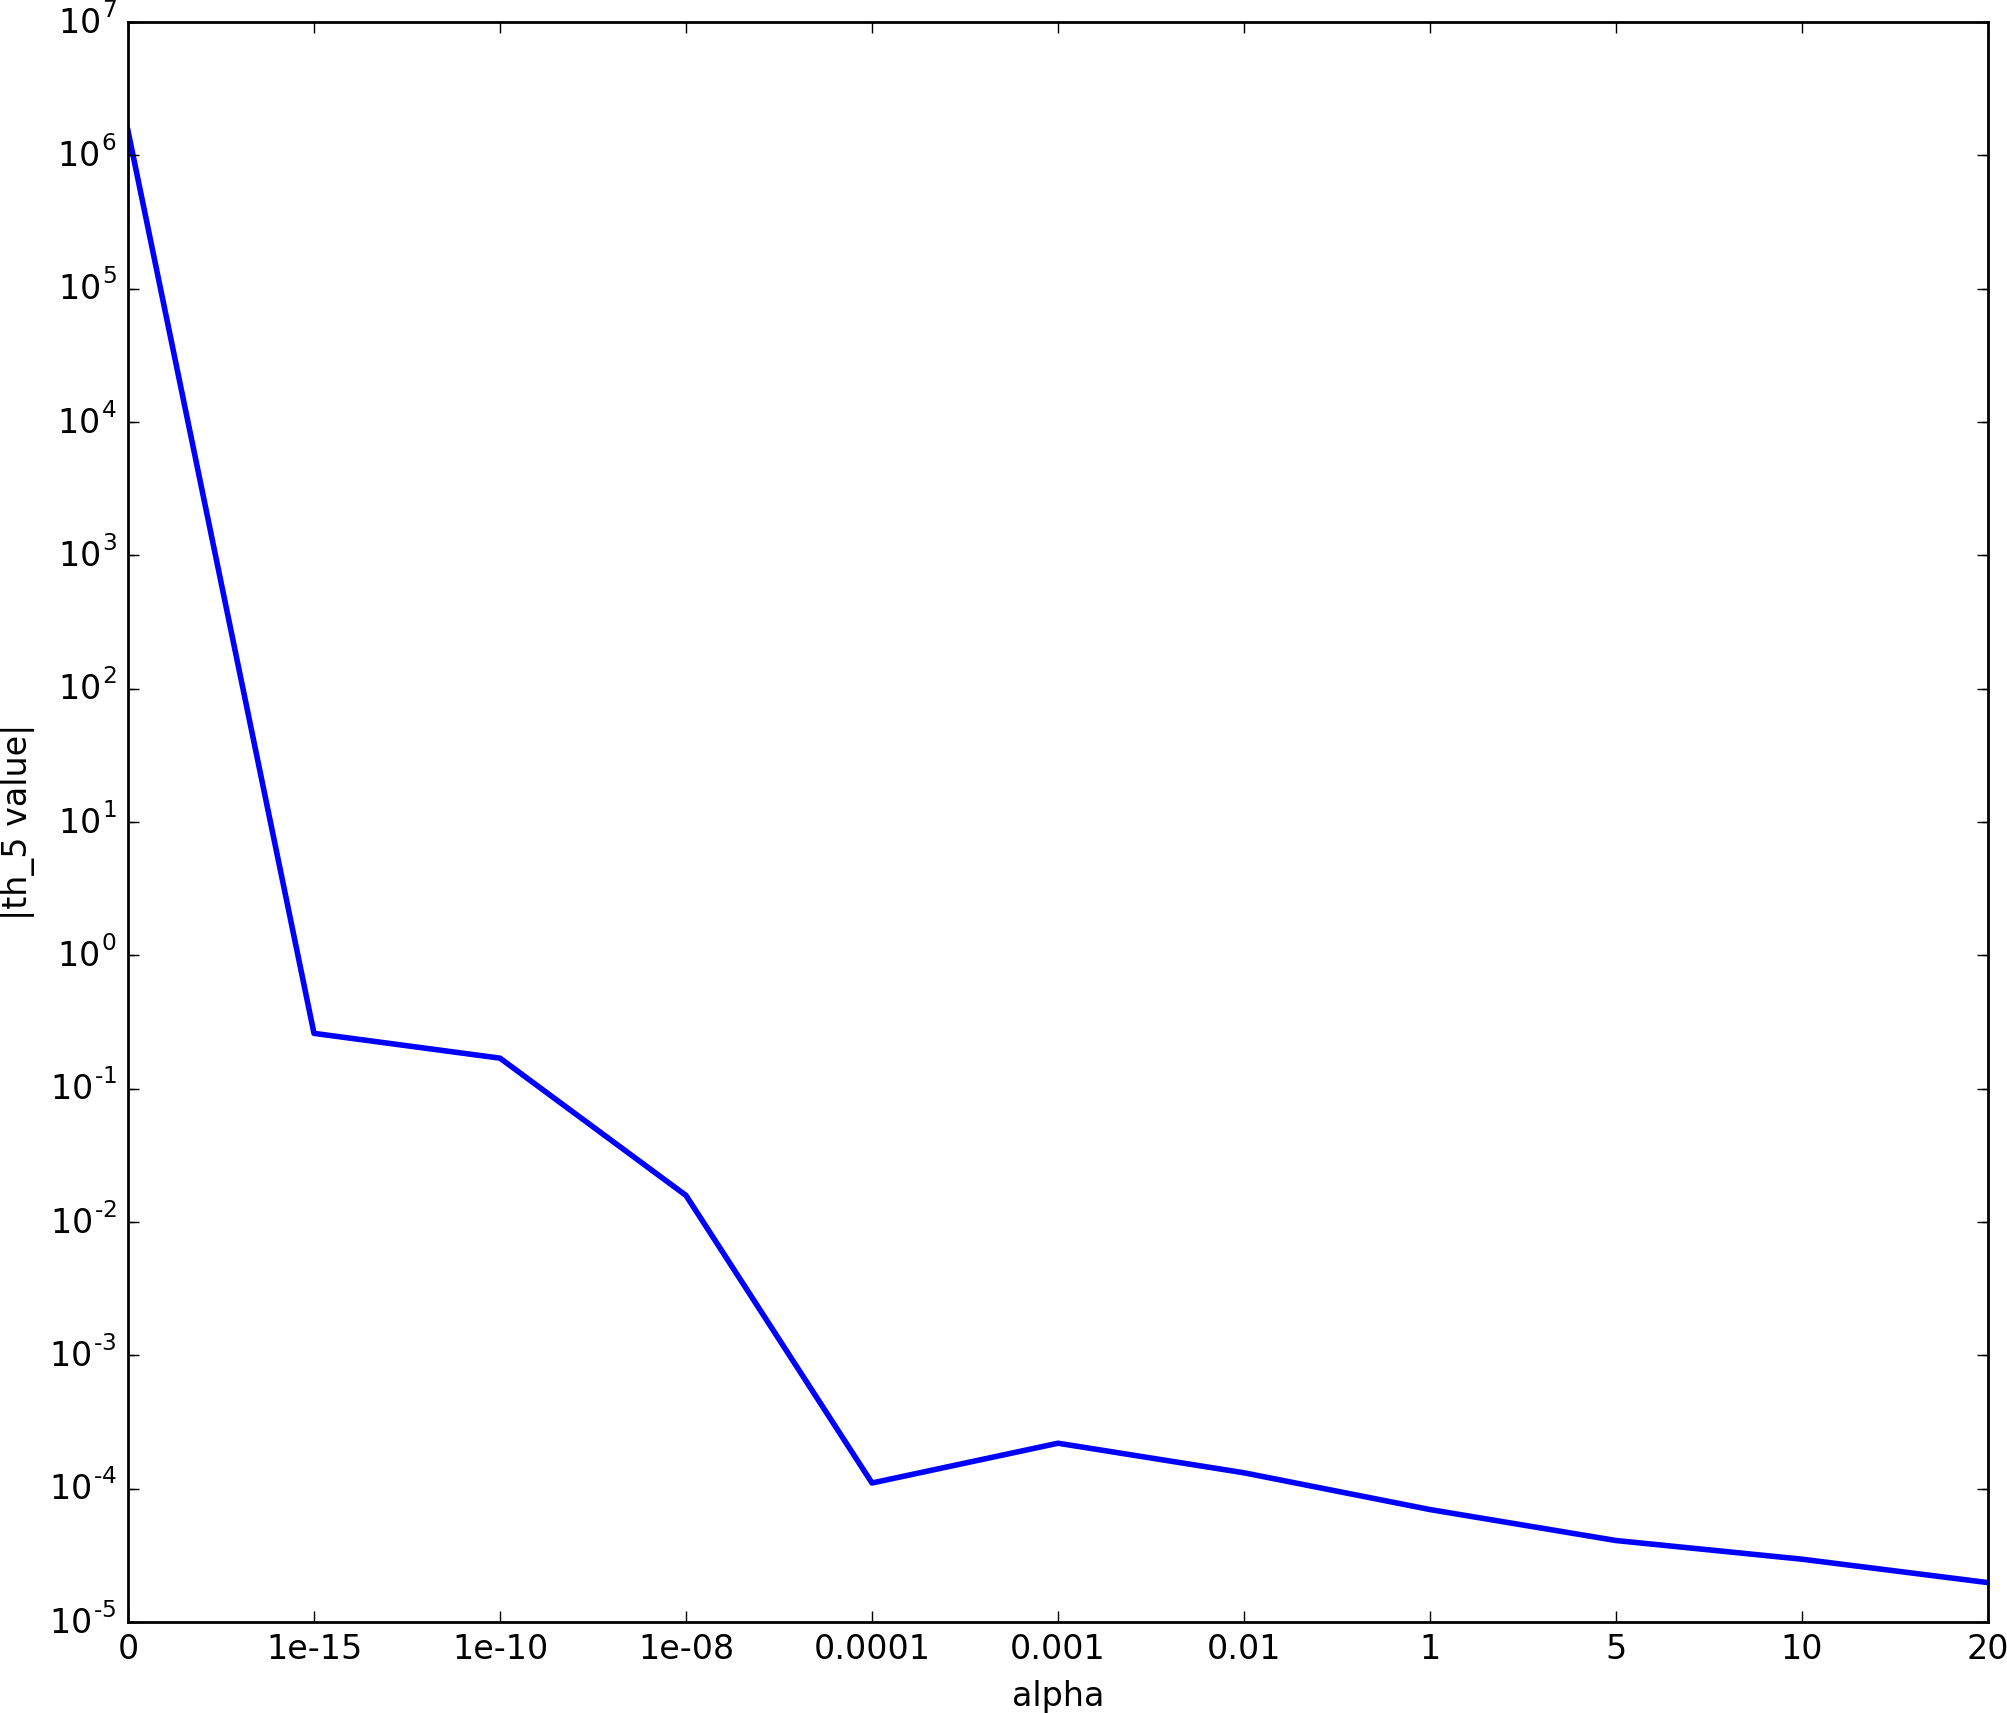
\includegraphics[height=0.4\textheight]{./fig/coefs_th5_ridge.png}\\
Value of $\theta_5$
\end{figure}
\end{frame}

%%%%%%%%%%%%%%%%%
\begin{frame}
\frametitle{Determination of the parameters in the ridge regression}
Considering the cost function J:
$$
J(\bm{\theta}) =J_{lms}(\bm{\theta}) + \alpha \sum_{i=0}^p \theta_i^2
$$
In a gradient algorithm, update of the parameters:

$\theta^{k+1}_i = \theta^k_i - \nu.(\frac{\partial J_{lms}}{D\theta_i} - 2\alpha\theta^k_i)$

So the update rule is:
$$
\theta^{k+1}_i = \theta^k_i(1-2 \nu \alpha) - \Delta_{lms}
$$
where
$\Delta_{lms}$ is the update in case of non-regularized regression

\end{frame}


%%%%%%%%%%%%%%%%%%%%
\begin{frame}
\frametitle{Lasso regression}
\begin{block}{}
Lasso regression is a linear regression with a Lasso regularization:
$$
J(\bm{\theta}) = \frac{1}{n} \sum (y_i - h_{\bm{\theta}}(x_i))^2 + \alpha \sum_{i=0}^p |\theta_i
$$
\end{block}
\end{frame}

%%%%%%%%%%%%%%%%%%%%
\begin{frame}
\frametitle{Results for $p=15$ and varying $\alpha$}
\begin{columns}
\column{.33\textwidth}
\vspace{-2em}
\begin{figure}
$\alpha=0$
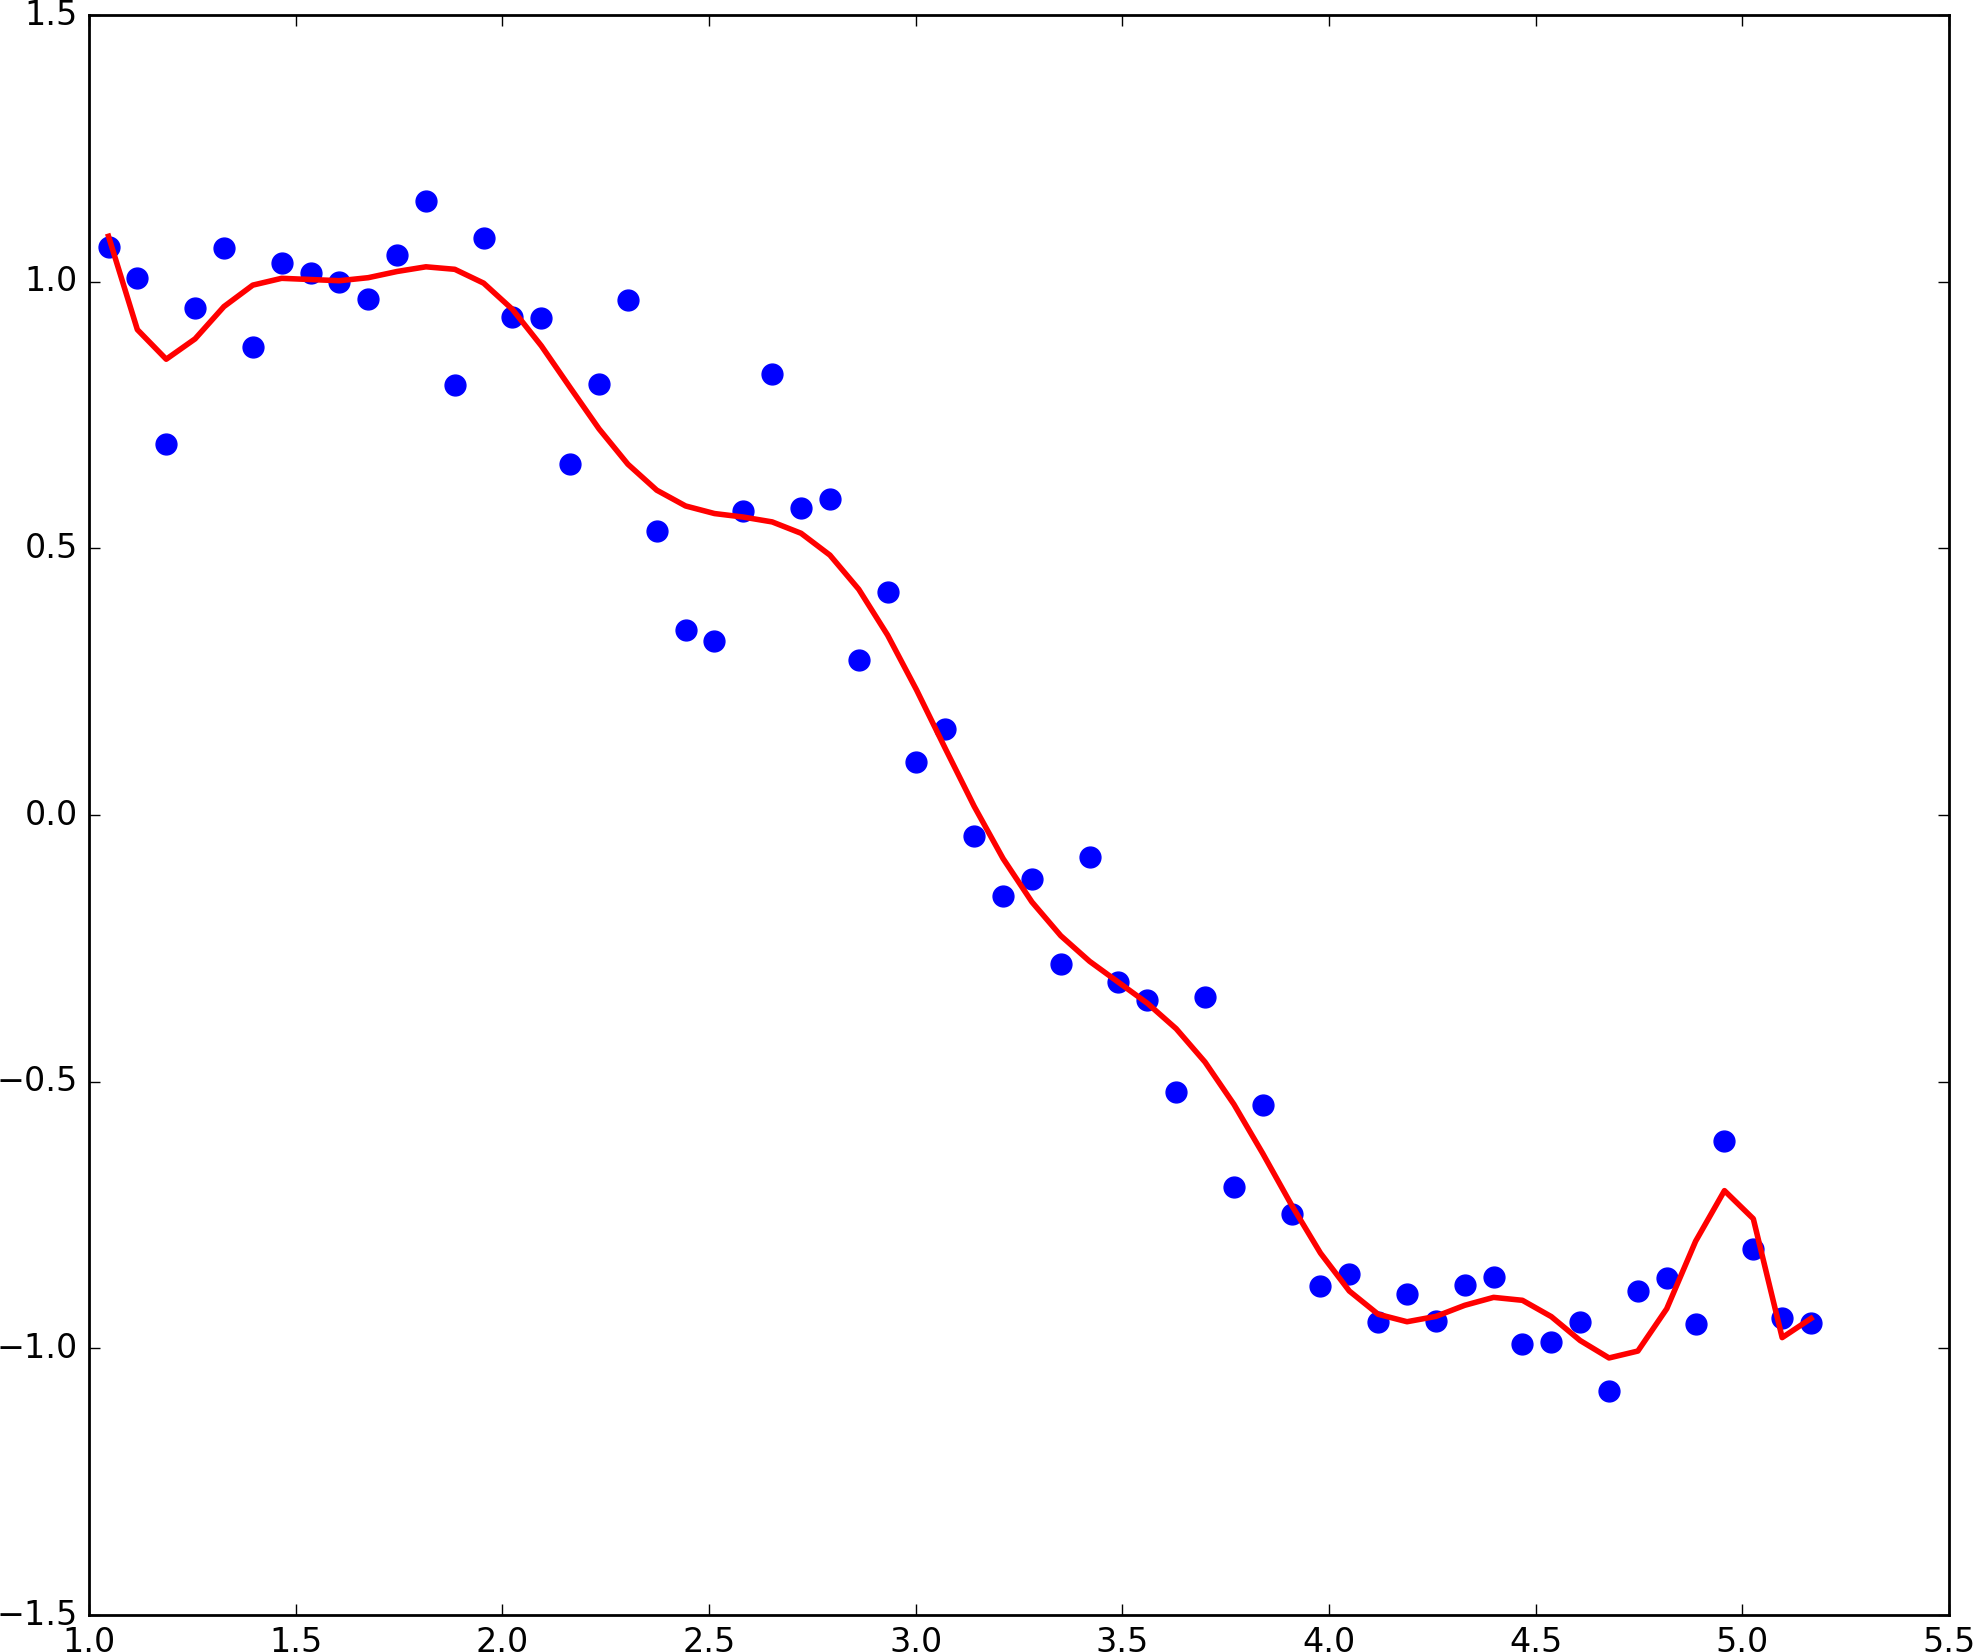
\includegraphics[width=0.99\textwidth]{./fig/lasso_alpha0.png}
\end{figure}
\vspace{-2em}
\begin{figure}
$\alpha=1e-3$
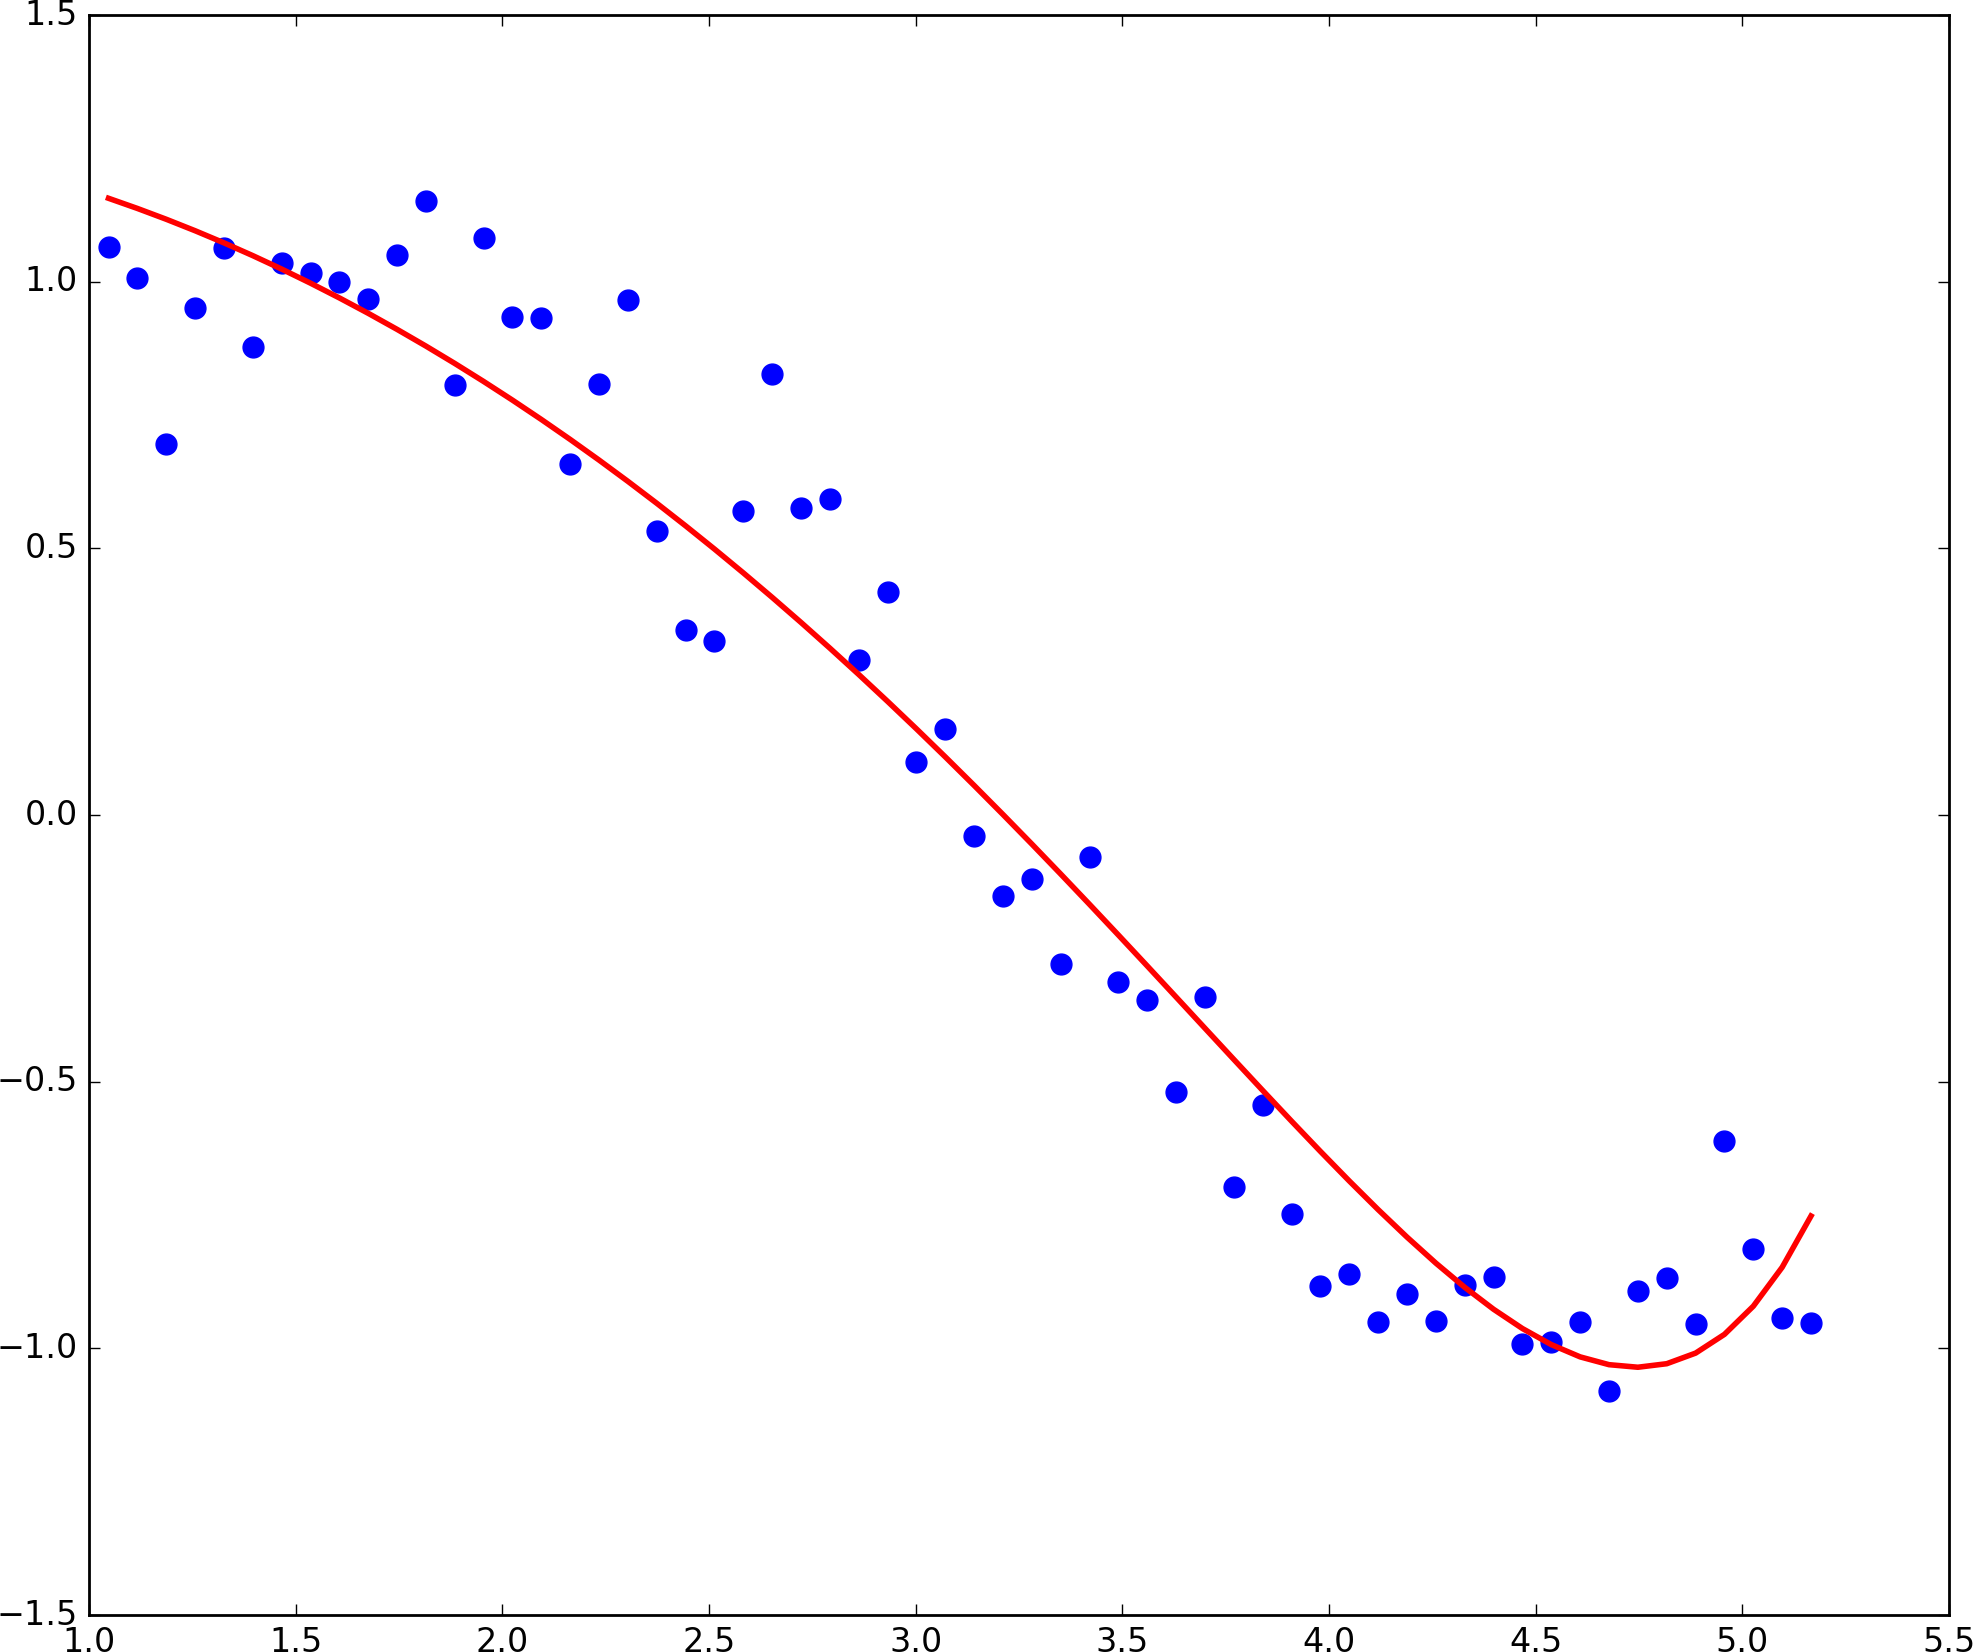
\includegraphics[width=0.99\textwidth]{./fig/lasso_alpha1e-3.png}
\end{figure}
\column{.33\textwidth}
\vspace{-2em}
\begin{figure}
$\alpha=1e-15$
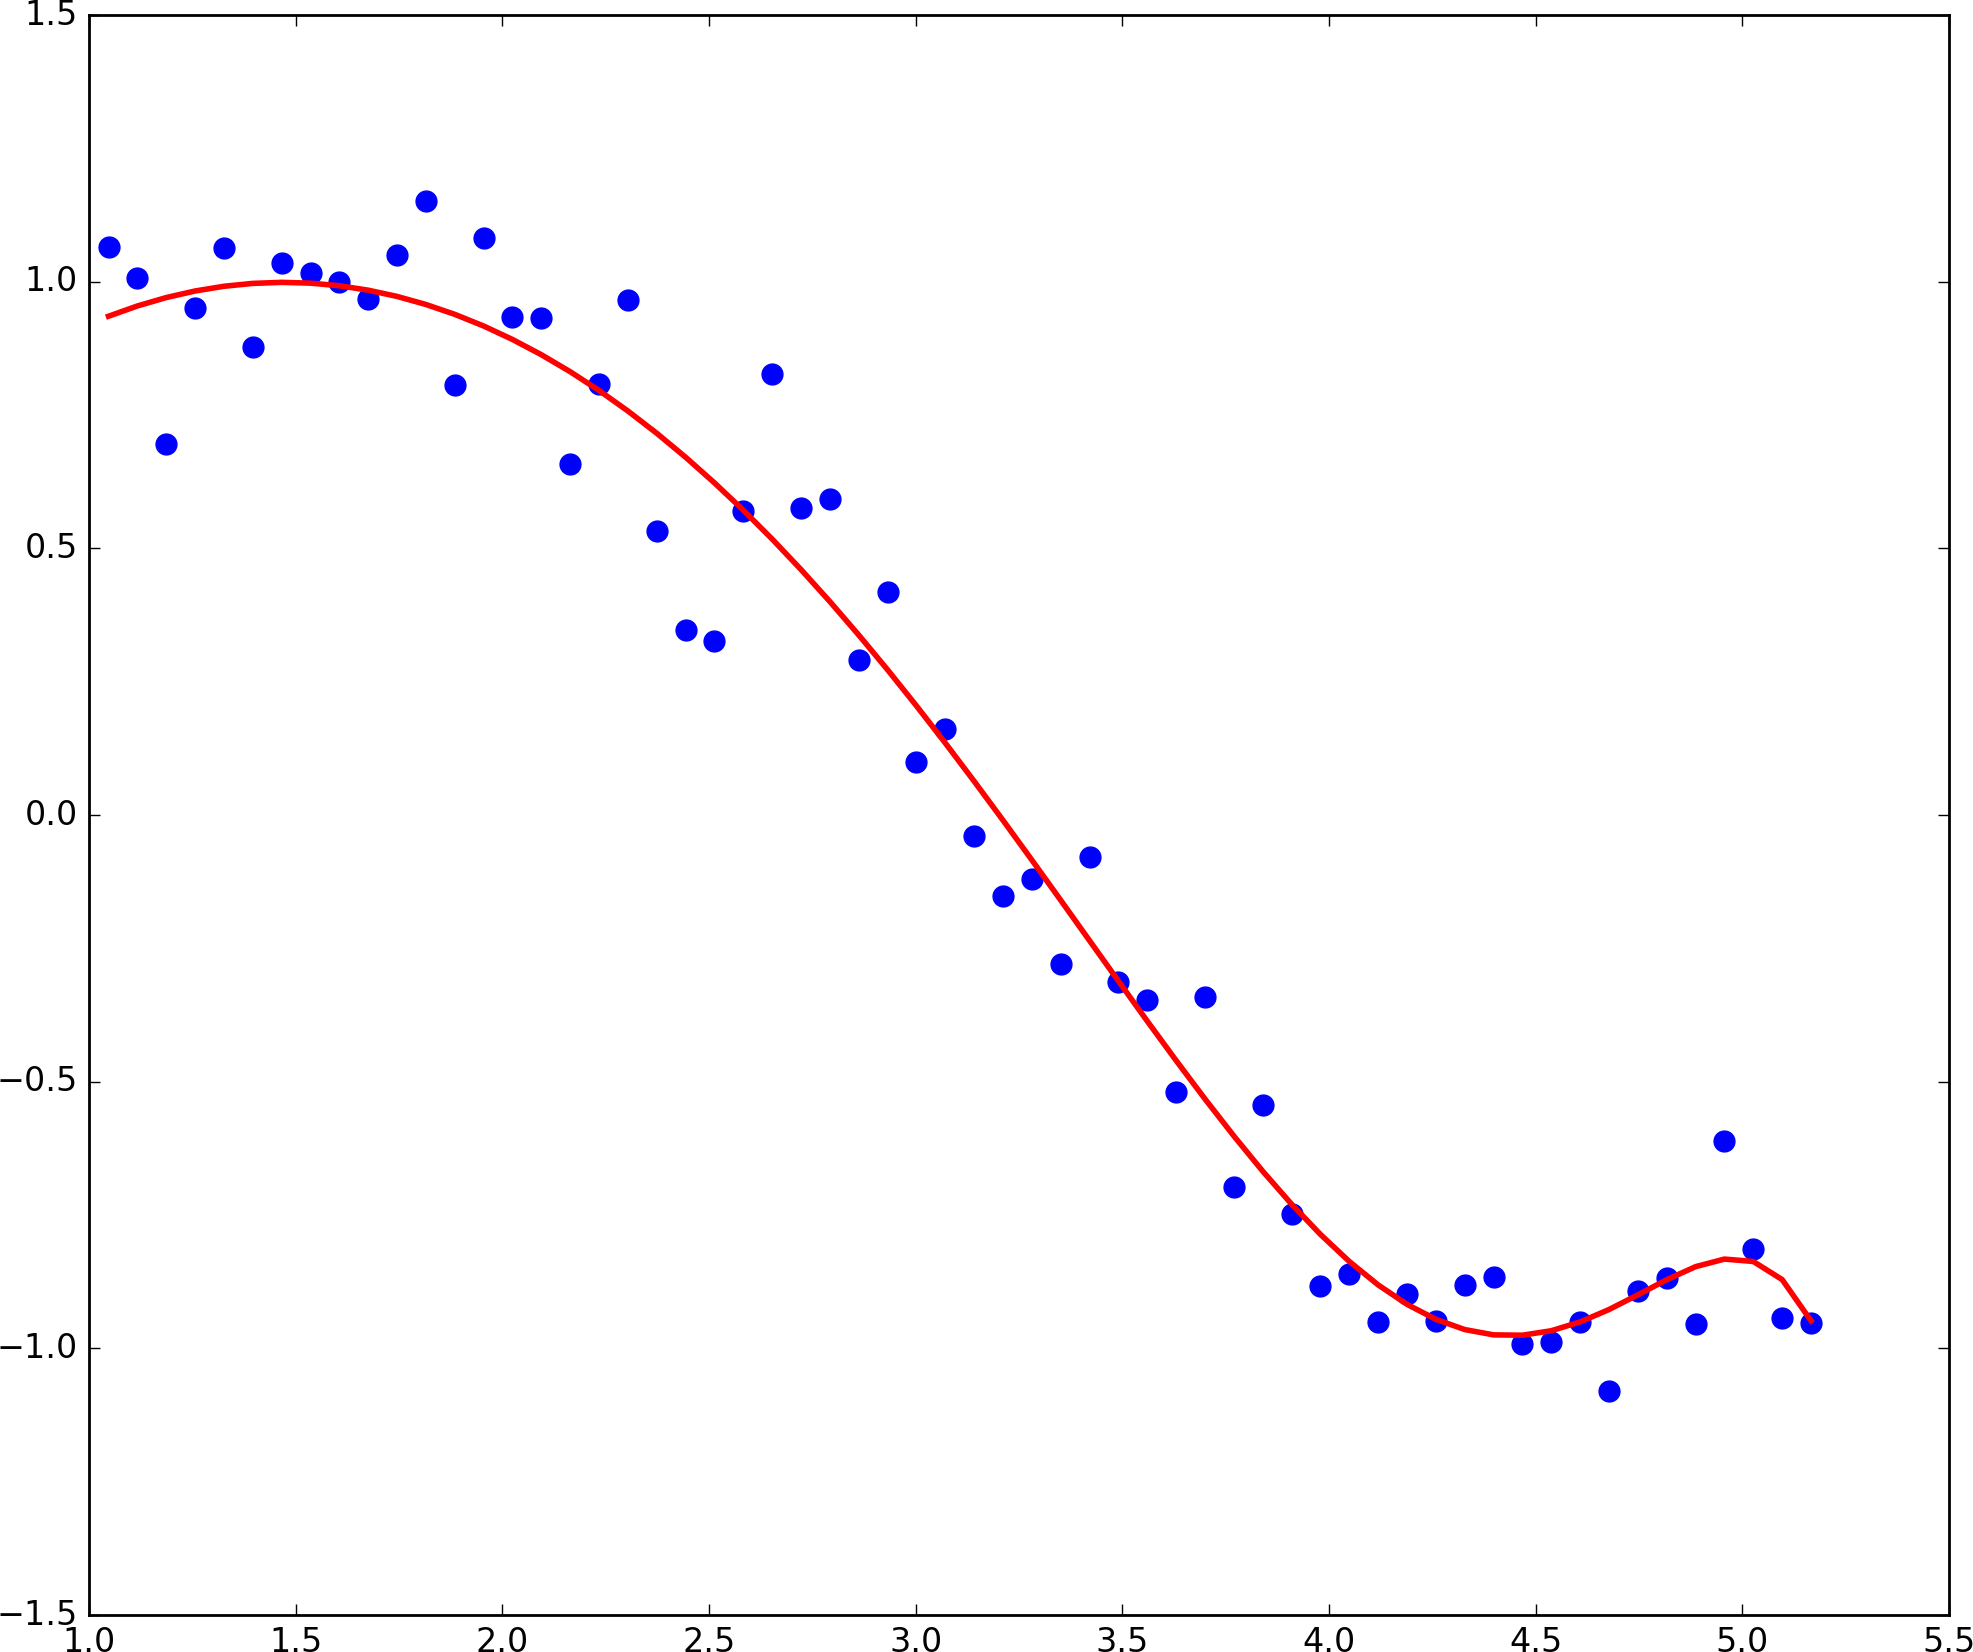
\includegraphics[width=0.99\textwidth]{./fig/lasso_alpha1e-15.png}
\end{figure}
\vspace{-2em}
\begin{figure}
$\alpha=1e-2$
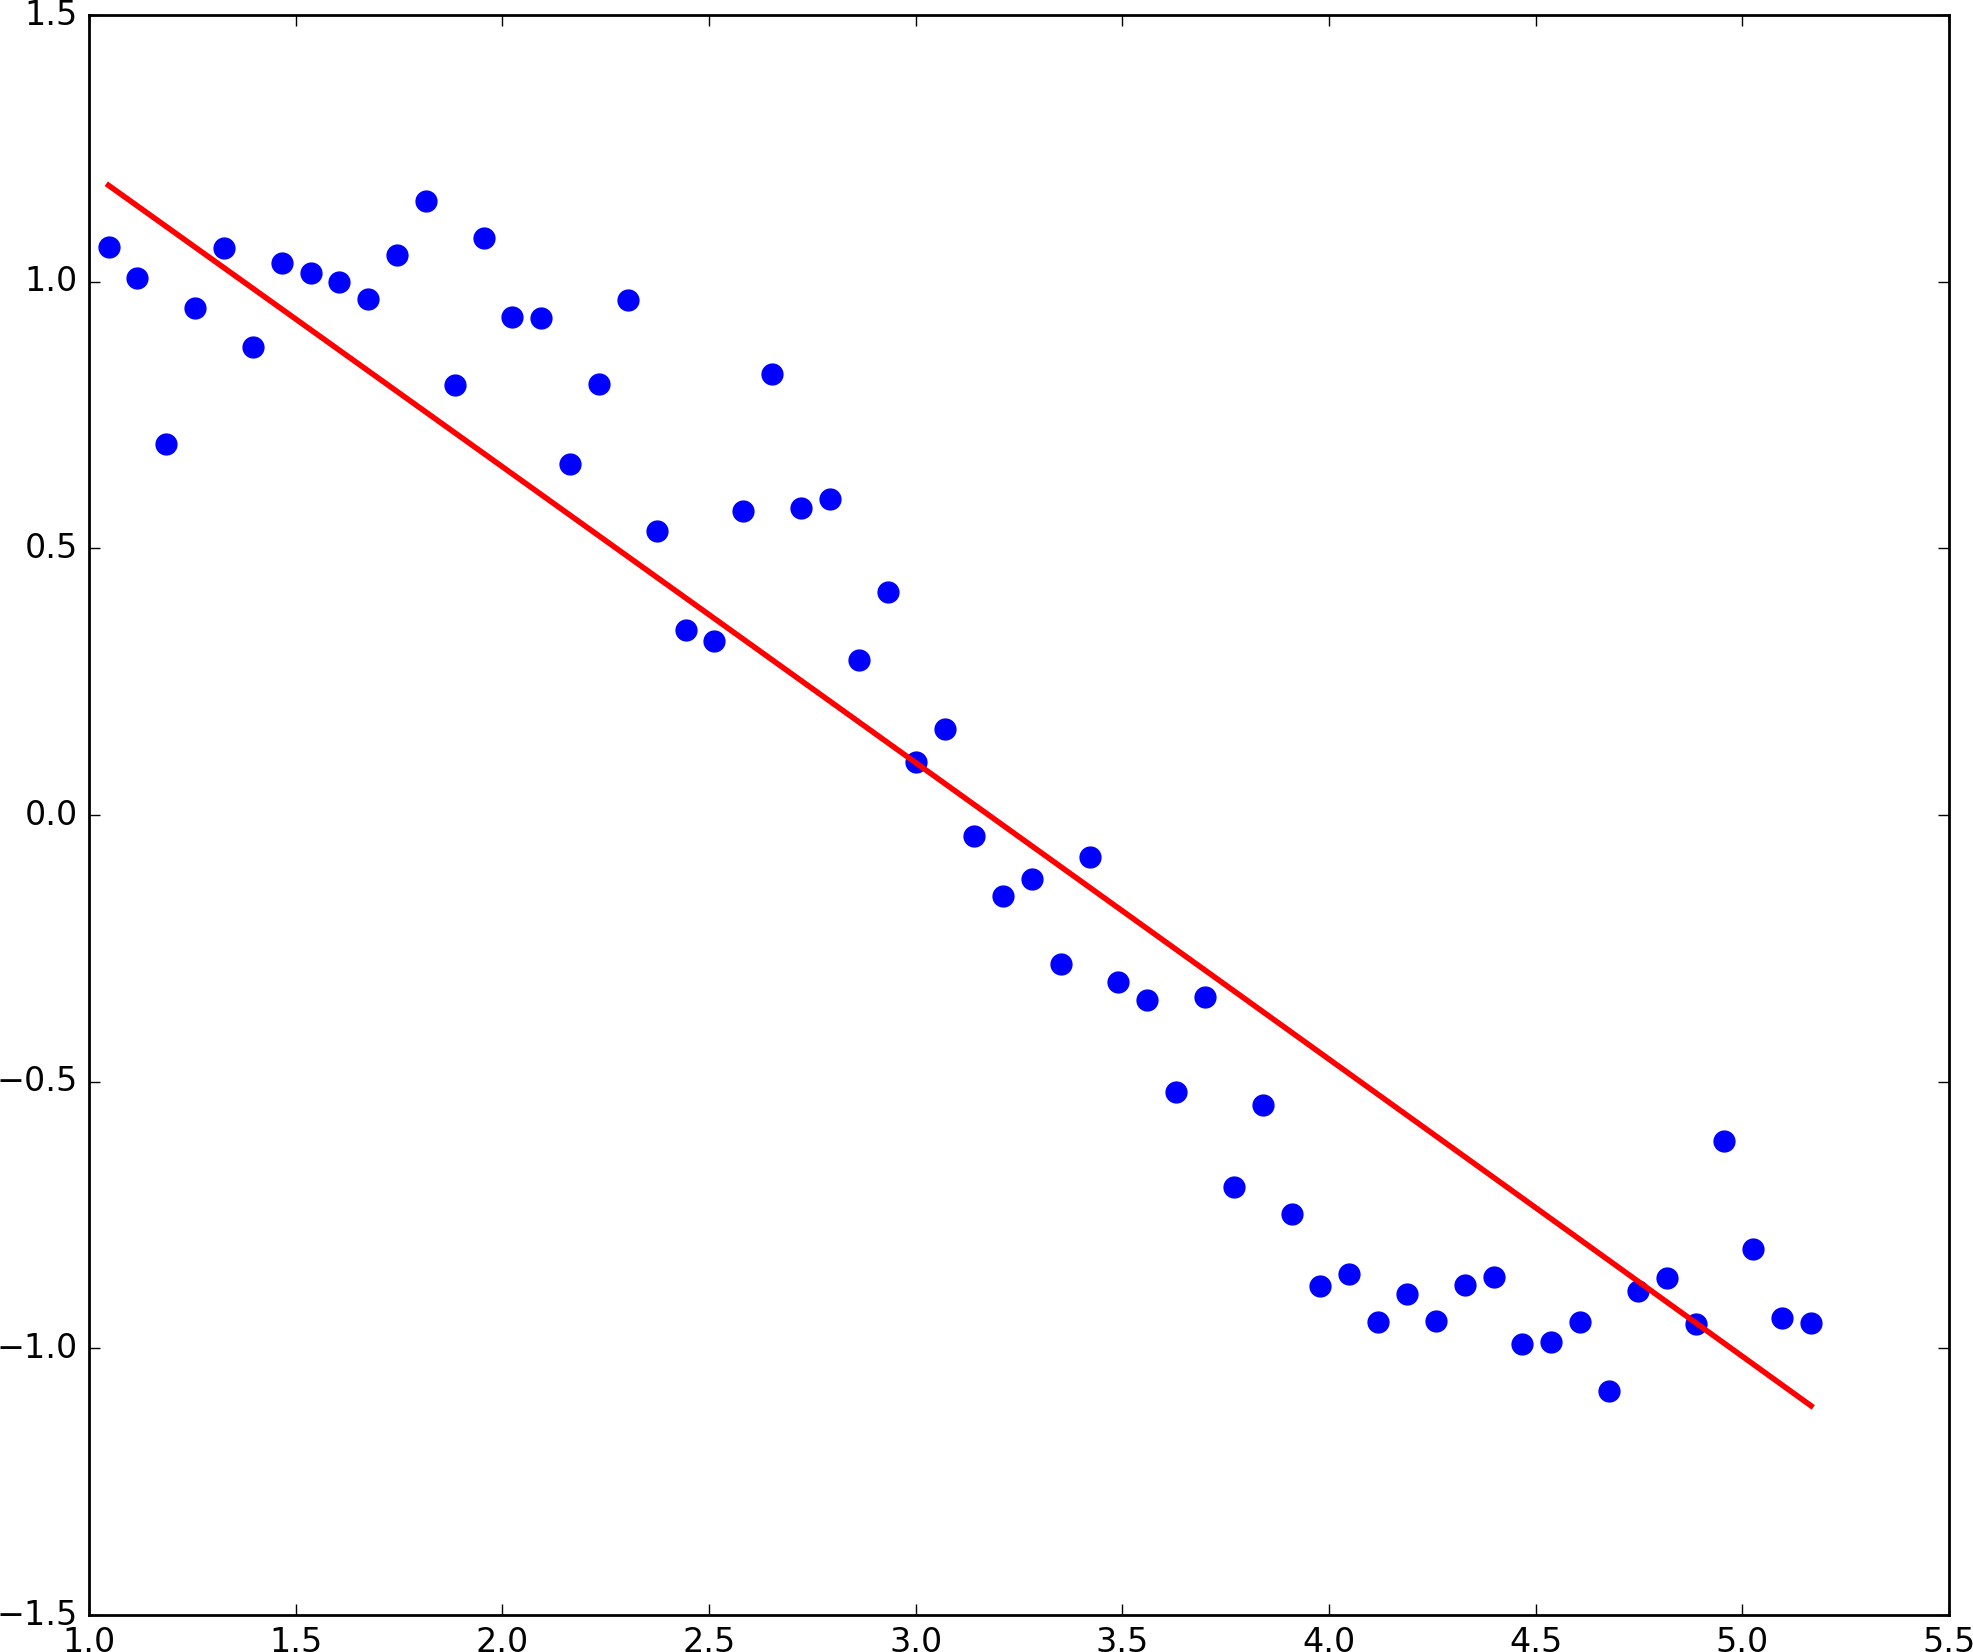
\includegraphics[width=0.99\textwidth]{./fig/lasso_alpha1e-2.png}
\end{figure}
\column{.33\textwidth}
\vspace{-2em}
\begin{figure}
$\alpha=1e-4$
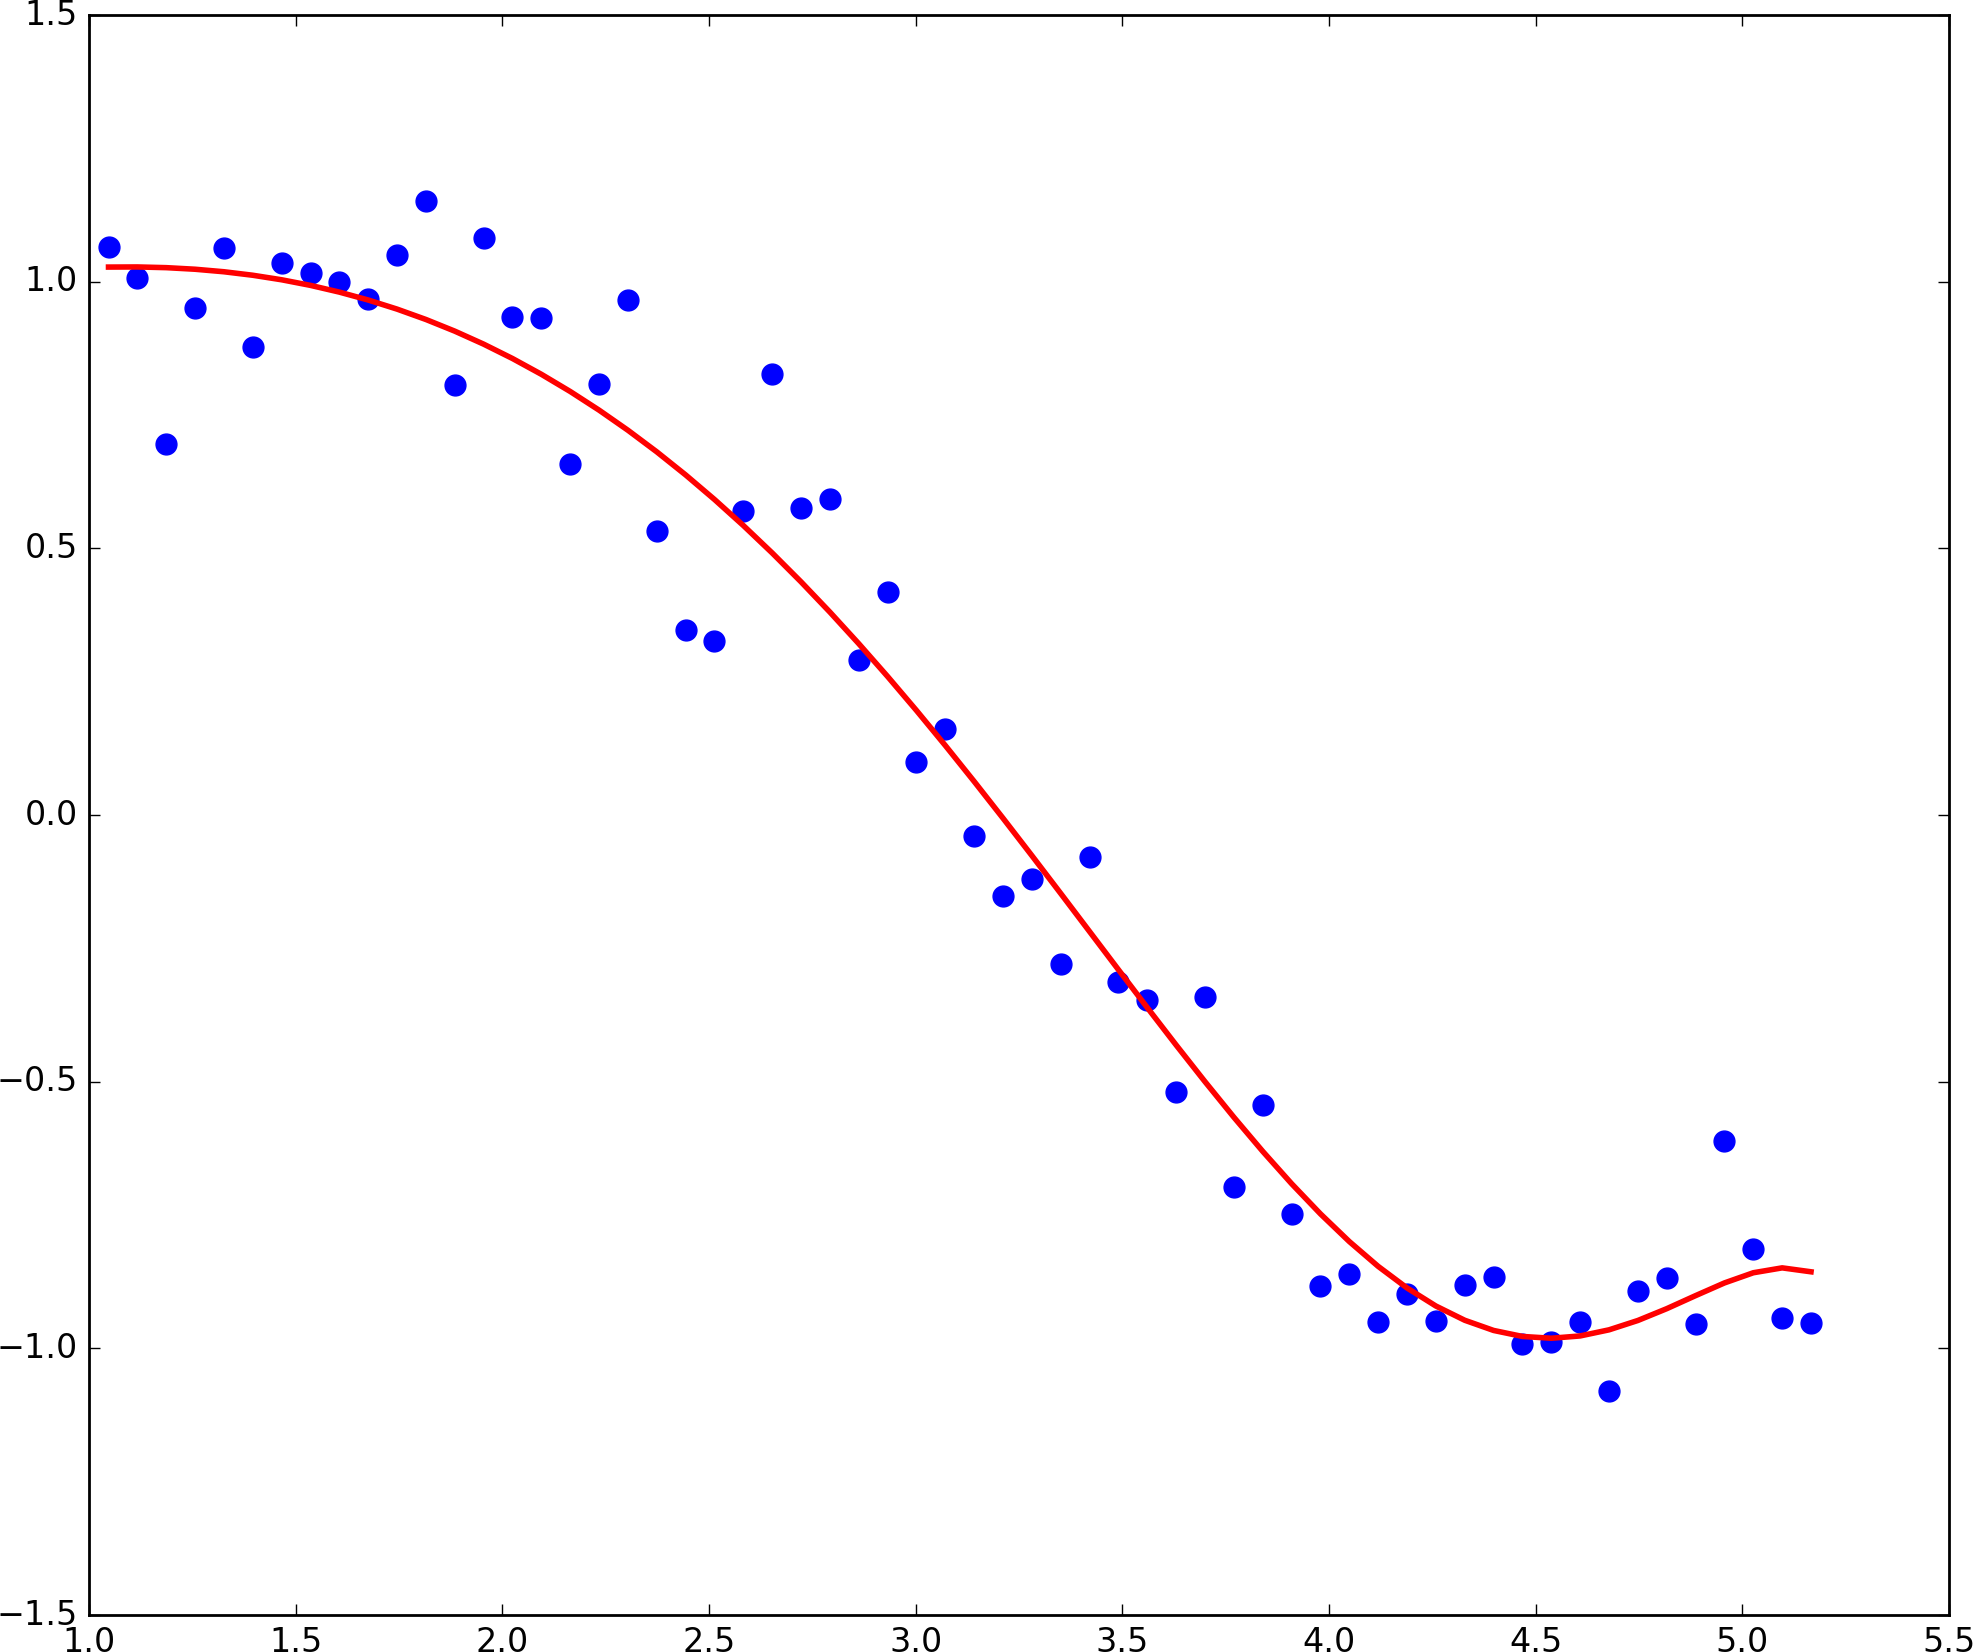
\includegraphics[width=0.99\textwidth]{./fig/lasso_alpha1e-4.png}
\end{figure}
\vspace{-2em}
\begin{figure}
$\alpha=5$
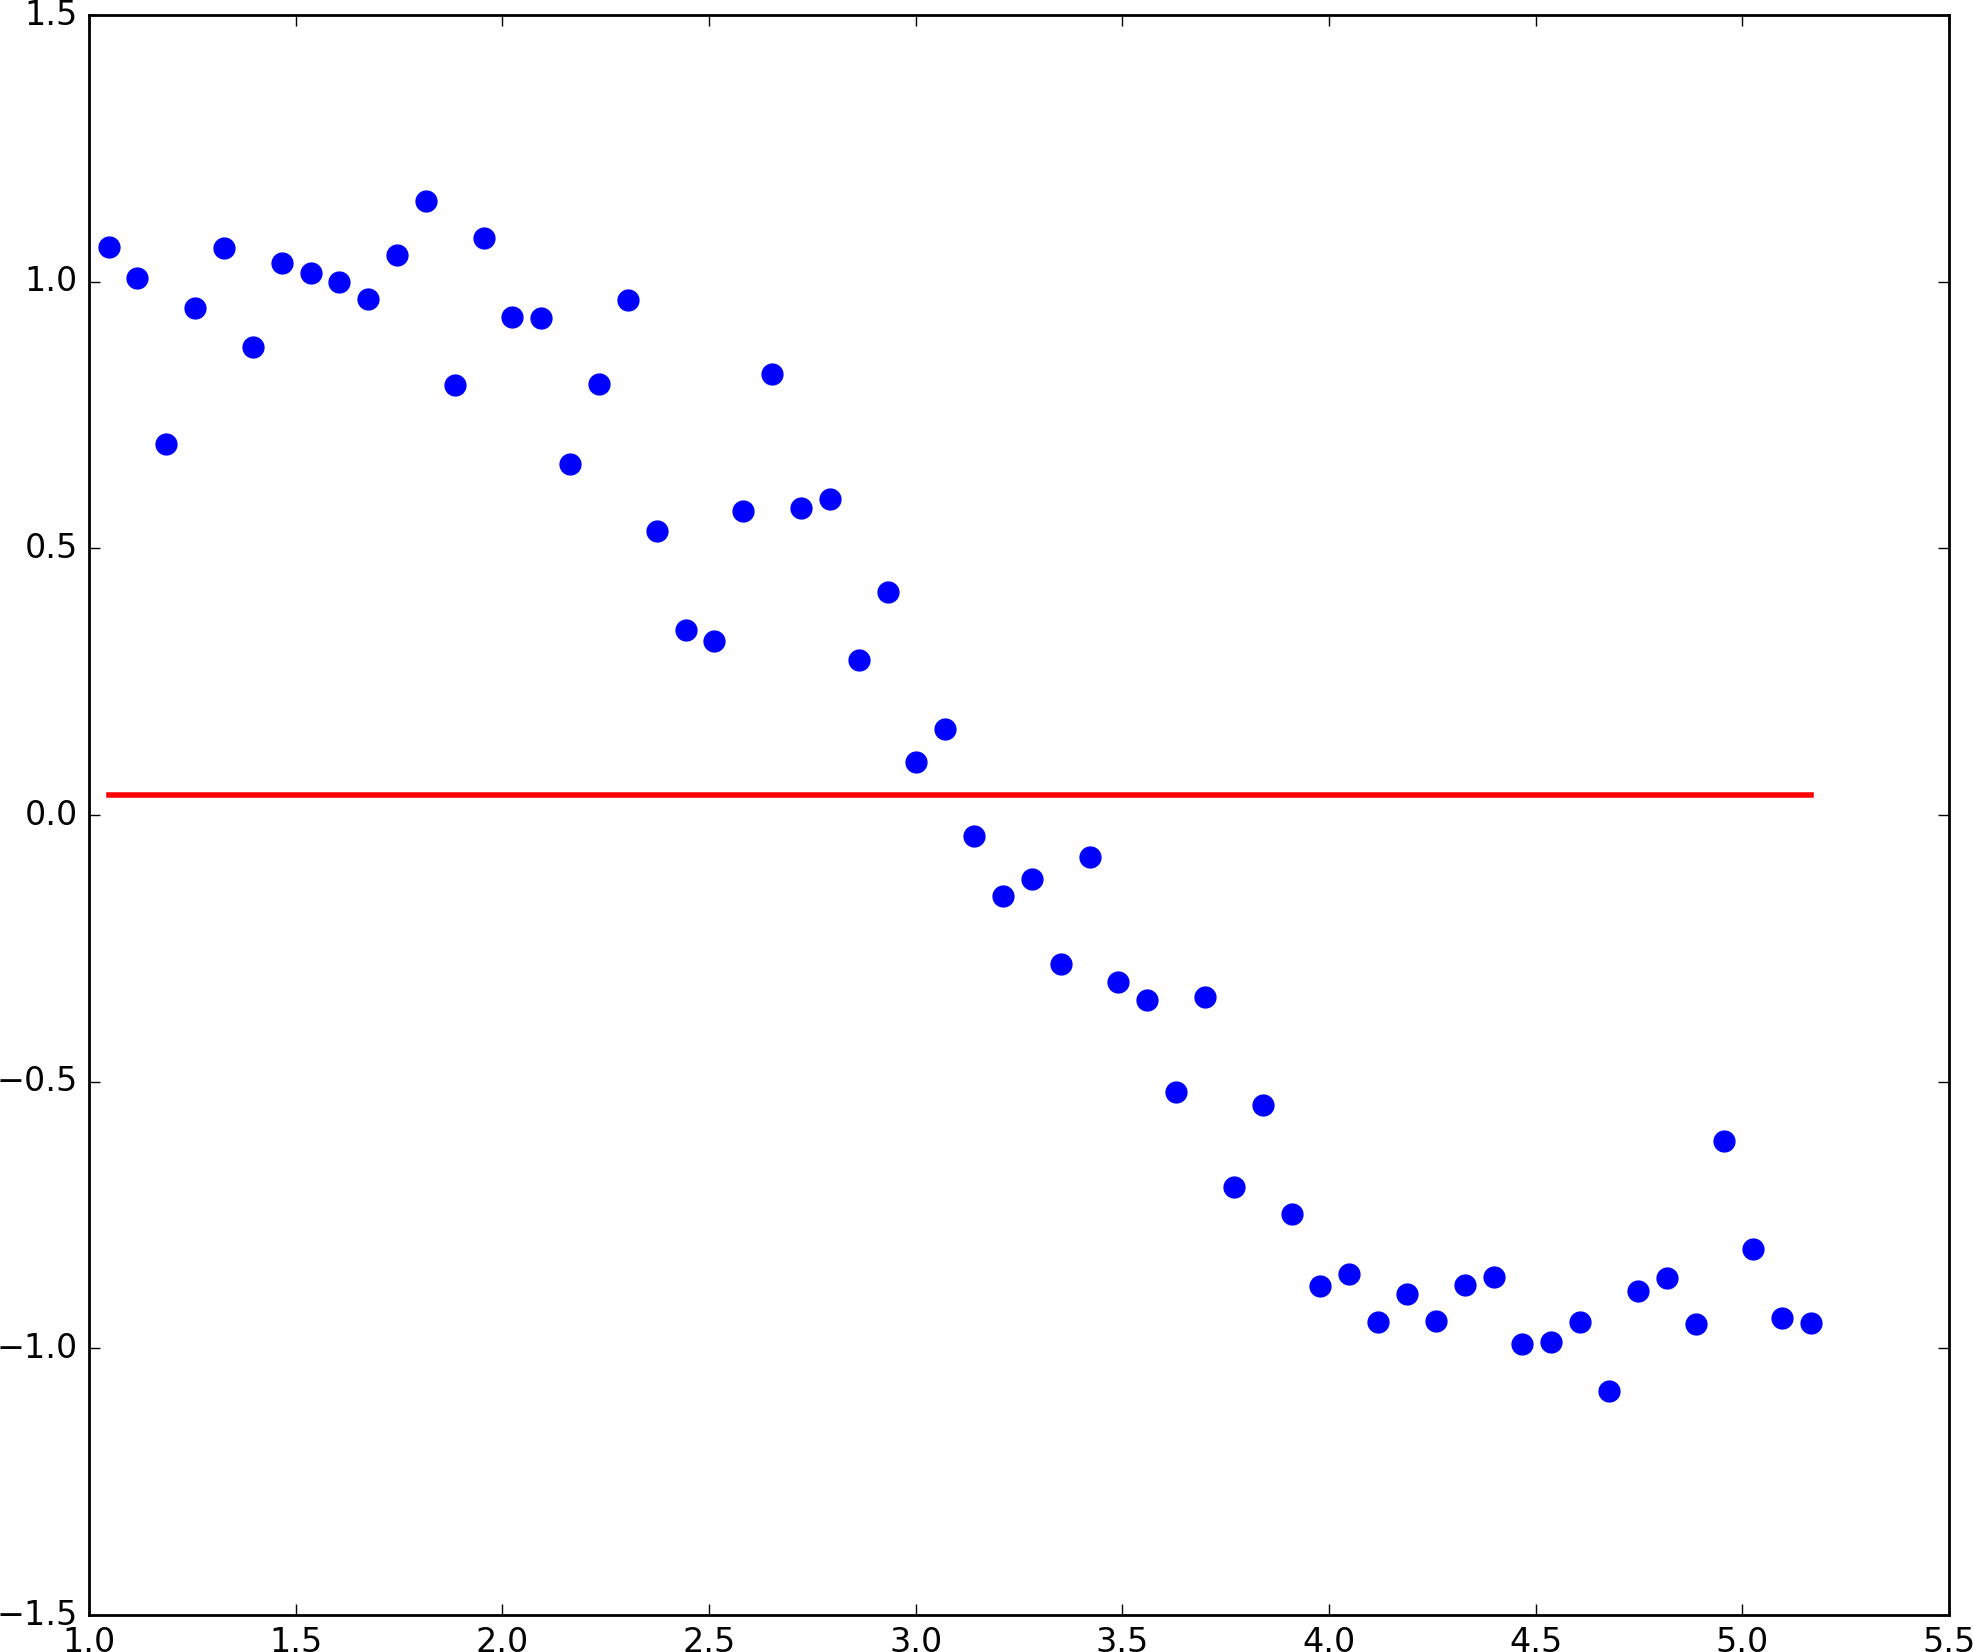
\includegraphics[width=0.99\textwidth]{./fig/lasso_alpha5.png}
\end{figure}
\end{columns}
\end{frame}

%%%%%%%%%%%%%%%%%%%%%
\begin{frame}
\frametitle{Values of coefficients}
\vspace{-2em}
\begin{table}
\resizebox{\textwidth}{!}{%
\begin{tabular}{lllllllllll}
\toprule
{} &      rmse &      th\_0 &      th\_1 &      th\_2 &      th\_3 &      th\_4 &      th\_5 &      th\_6 &      th\_7 &      th\_8 \\
\midrule
alpha\_0      & +1.17e-02 & -3.62e+04 & +2.44e+05 & -7.46e+05 & +1.38e+06 & -1.71e+06 & +1.53e+06 & -1.00e+06 & +4.98e+05 & -1.88e+05 \\
alpha\_1e-15  & +1.59e-02 & +2.22e-01 & +1.06e+00 & -3.69e-01 & +8.85e-04 & +1.63e-03 & -1.19e-04 & -6.44e-05 & -6.28e-06 & +1.45e-06 \\
alpha\_1e-10  & +1.59e-02 & +2.22e-01 & +1.06e+00 & -3.69e-01 & +8.84e-04 & +1.63e-03 & -1.18e-04 & -6.44e-05 & -6.28e-06 & +1.45e-06 \\
alpha\_1e-08  & +1.59e-02 & +2.22e-01 & +1.06e+00 & -3.69e-01 & +7.69e-04 & +1.62e-03 & -1.10e-04 & -6.45e-05 & -6.32e-06 & +1.43e-06 \\
alpha\_0.0001 & +1.72e-02 & +9.03e-01 & +1.71e-01 & -0.00e+00 & -4.78e-02 & -0.00e+00 & -0.00e+00 & +0.00e+00 & +0.00e+00 & +9.47e-06 \\
alpha\_0.001  & +2.80e-02 & +1.29e+00 & -0.00e+00 & -1.26e-01 & -0.00e+00 & -0.00e+00 & -0.00e+00 & +0.00e+00 & +0.00e+00 & +0.00e+00 \\
alpha\_0.01   & +6.07e-02 & +1.76e+00 & -5.52e-01 & -5.62e-04 & -0.00e+00 & -0.00e+00 & -0.00e+00 & -0.00e+00 & -0.00e+00 & -0.00e+00 \\
alpha\_1      & +6.16e-01 & +3.80e-02 & -0.00e+00 & -0.00e+00 & -0.00e+00 & -0.00e+00 & -0.00e+00 & -0.00e+00 & -0.00e+00 & -0.00e+00 \\
alpha\_5      & +6.16e-01 & +3.80e-02 & -0.00e+00 & -0.00e+00 & -0.00e+00 & -0.00e+00 & -0.00e+00 & -0.00e+00 & -0.00e+00 & -0.00e+00 \\
alpha\_10     & +6.16e-01 & +3.80e-02 & -0.00e+00 & -0.00e+00 & -0.00e+00 & -0.00e+00 & -0.00e+00 & -0.00e+00 & -0.00e+00 & -0.00e+00 \\
alpha\_20     & +6.16e-01 & +3.80e-02 & -0.00e+00 & -0.00e+00 & -0.00e+00 & -0.00e+00 & -0.00e+00 & -0.00e+00 & -0.00e+00 & -0.00e+00 \\
\bottomrule
\end{tabular}
}
\end{table}
\begin{figure}
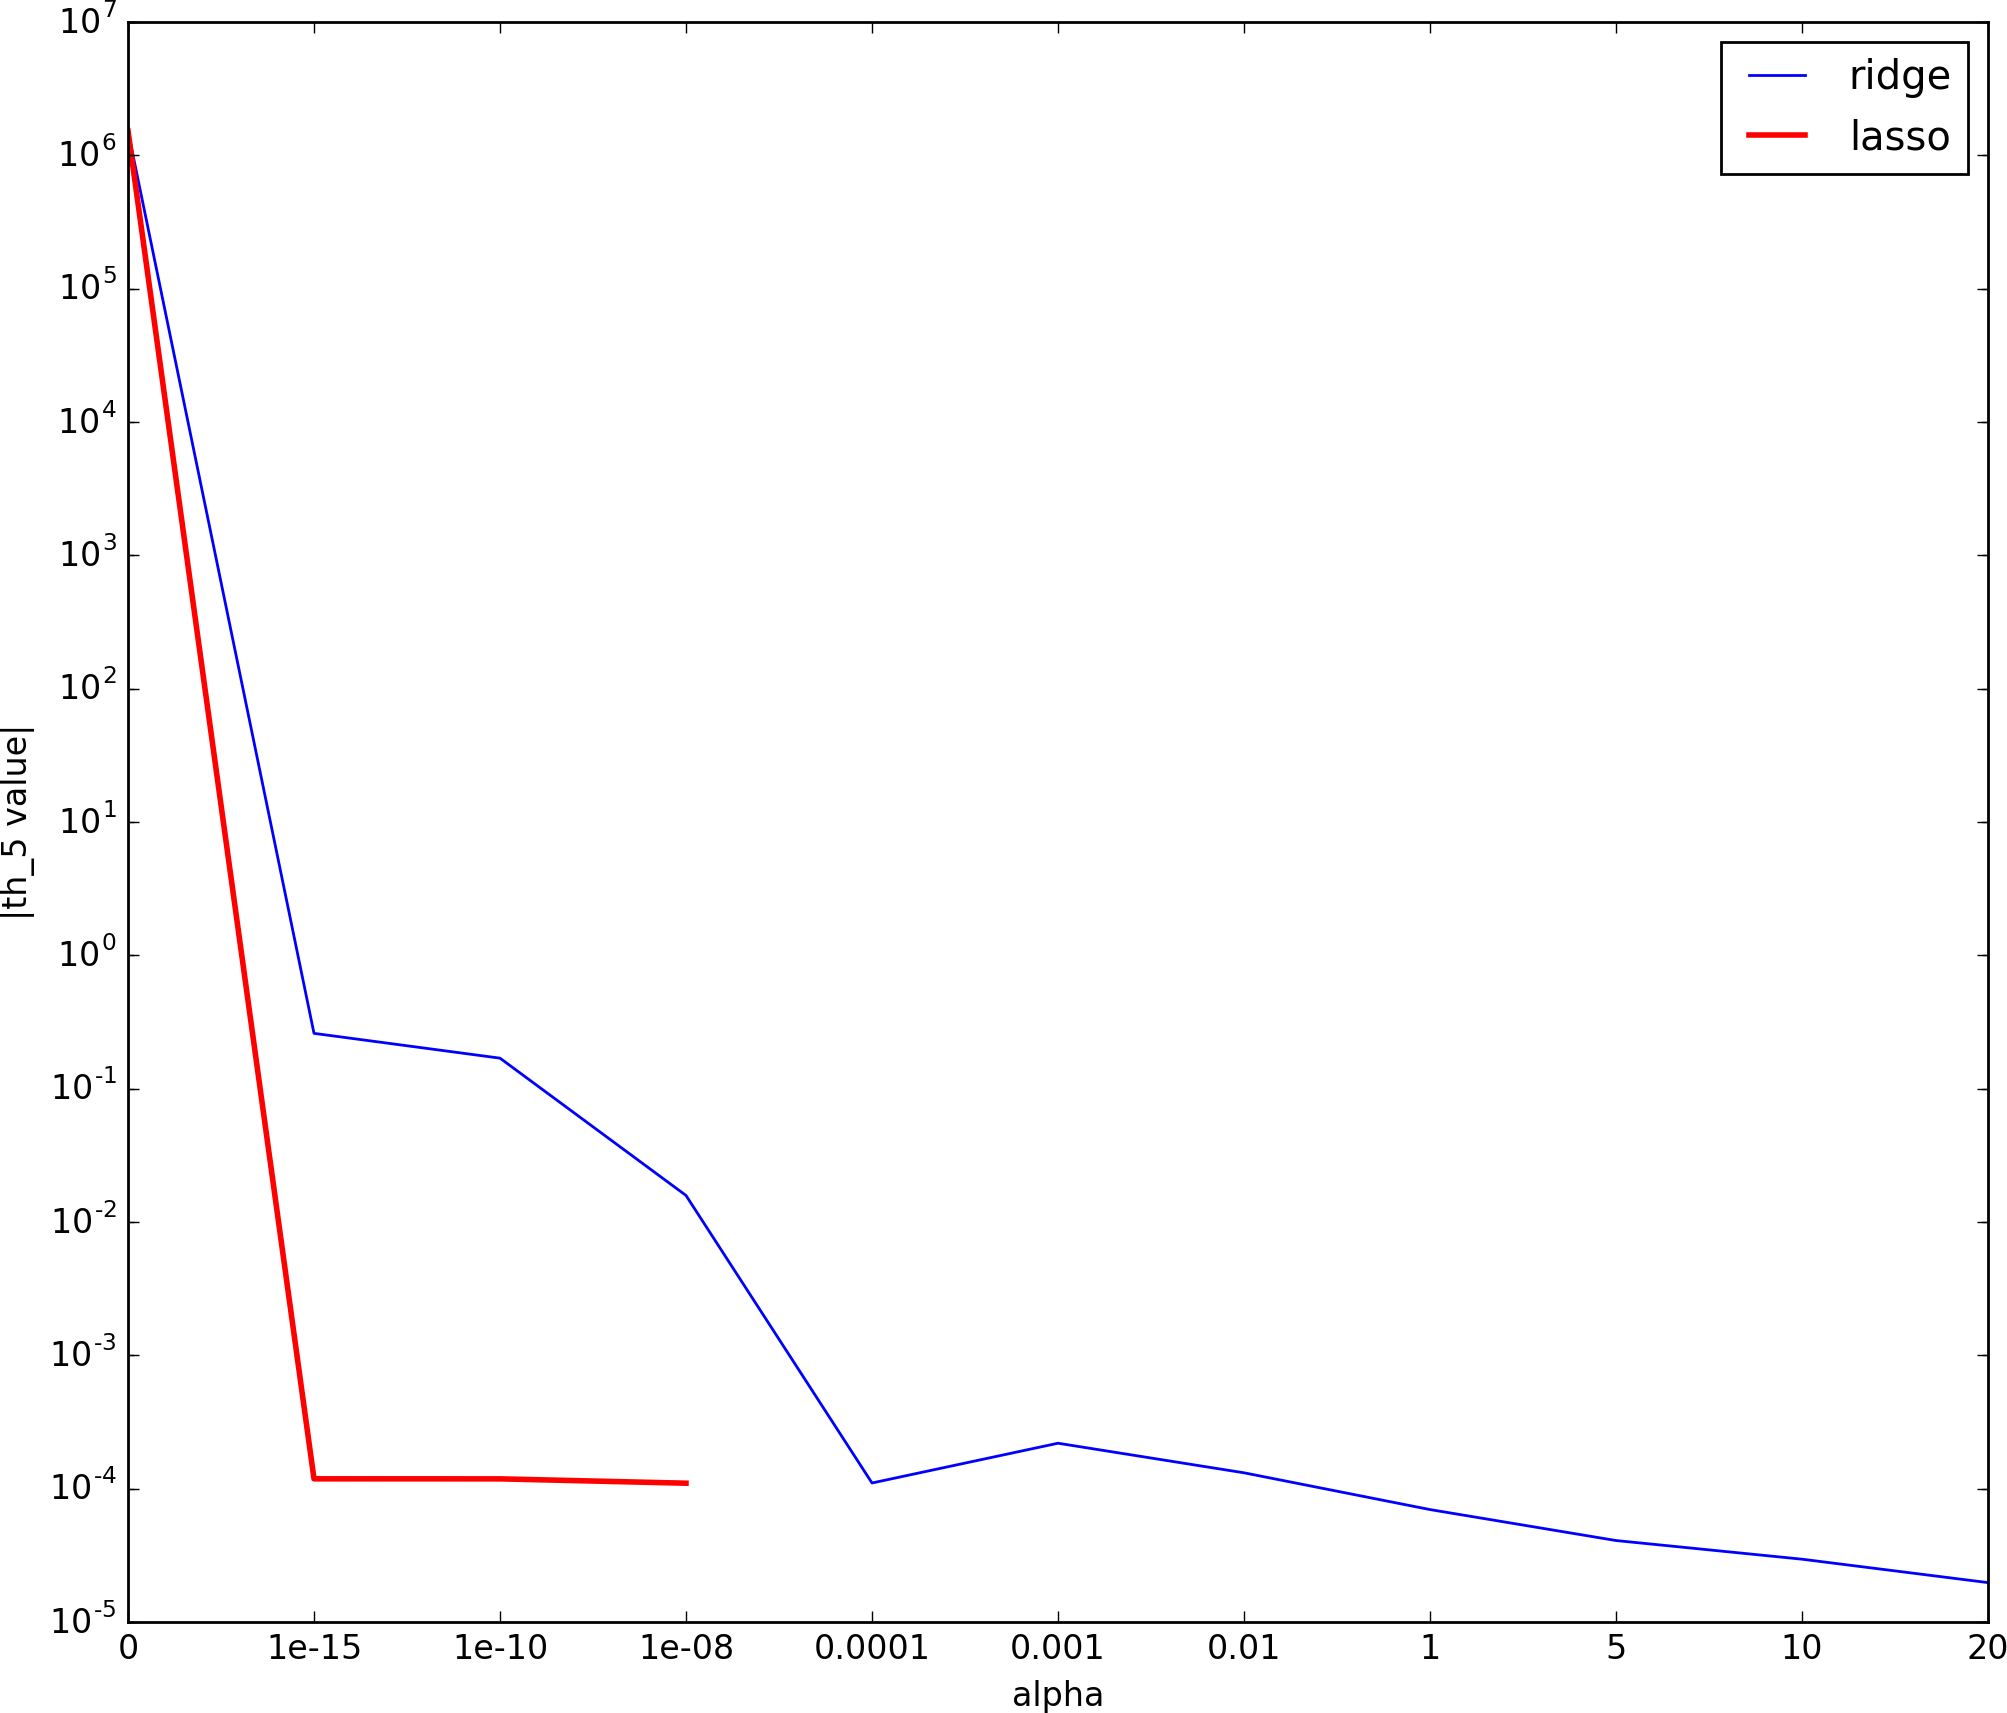
\includegraphics[height=0.4\textheight]{./fig/coefs_th5_lasso.png}\\
Value of $\theta_5$
\end{figure}
\end{frame}

%%%%%%%%%%%%%%%%%%%%
\begin{frame}
\frametitle{Determination of the parameters in the lasso regression}
Considering the cost function J:
$$
J(\bm{\theta}) =J_{lms}(\bm{\theta}) + \alpha \sum_{i=0}^p |\theta_i|
$$
In a gradient algorithm, update of the parameters would be:

J is not differentiable.
If we consider $\theta_{lms} = \theta_i^k -\nu.\frac{\partial J_{lms}}{D\theta_i} $

The update rule is:
\begin{itemize}
\item $\theta_i^{k+1} = \theta_{lms} + \alpha \nu$  if $\theta_{lms} < -\alpha \nu$
\item $\theta_i^k = 0$ if $-\alpha \nu < \theta_{lms} < \alpha \nu$
\item $\theta_i^{k+1} = \theta_{lms} - \alpha \nu$  if $\theta_{lms} > \alpha \nu$
\end{itemize}
\end{frame}

%%%%%%%%%%%%%%%%%%%%
\begin{frame}
\frametitle{Summary of parameters updates}
\begin{figure}
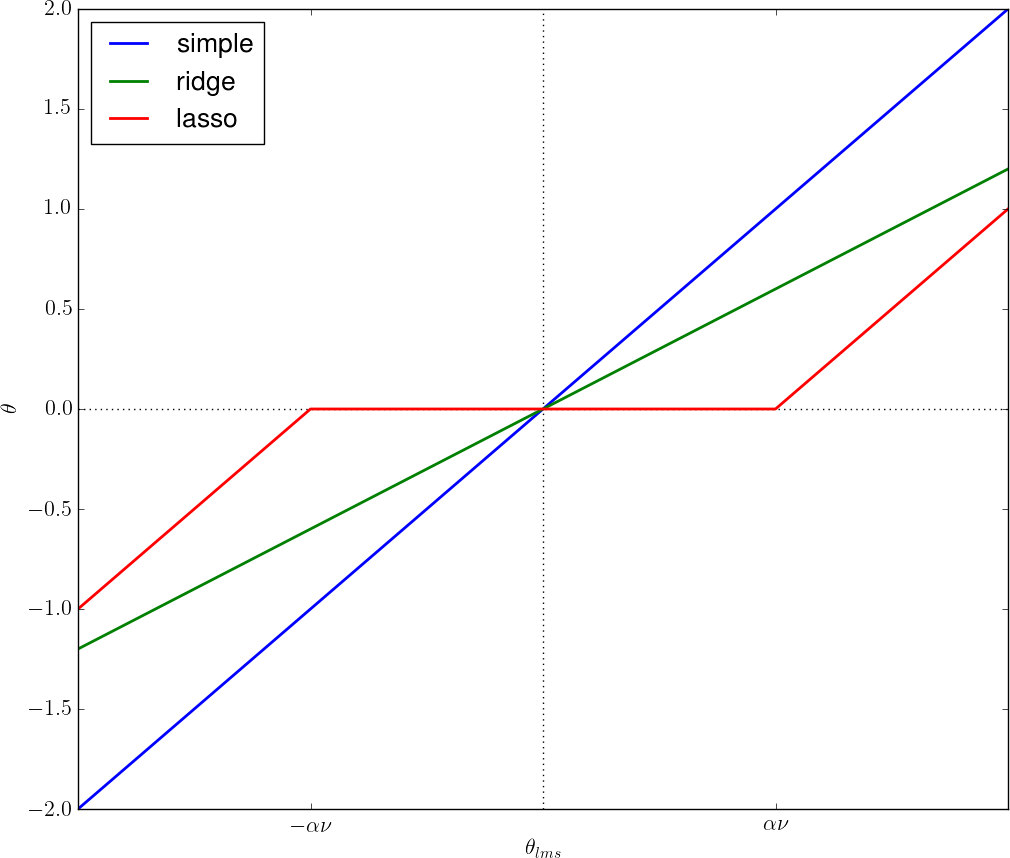
\includegraphics[height=0.8\textheight]{./fig/updates.png}
\end{figure}
\end{frame}

%%%%%%%%%%%%%%%%%%%%%
\begin{frame}
\frametitle{Comparison Ridge/Lasso}
\begin{exampleblock}{ridge}
\begin{itemize}
\item Prevents the overfitting
\item includes all the features (dimensions) of the predictor, 
so it can be useless for high dimensional predictors
\end{itemize}
\end{exampleblock}
\pause
\begin{alertblock}{lasso}
\begin{itemize}
\item Provides sparse solutions and reduce the dimension of the
predictor
\item If some features in the predictor are correlated, arbitrarily select
one from the others.
\end{itemize}
\end{alertblock}
\end{frame}
%%%%%%%%%%%%%%%%%%%%%
\begin{frame}
\frametitle{Model Selection}
\begin{alertblock}{The "big" question}
How to determine some "hyper-parameter" of our model ?

examples: $\alpha$ for regularization, degree of polynomials
\end{alertblock}
\pause
The common approach:
\begin{enumerate}[<+->]
\item Split the dataset in two dataset : training and test
\item Optimize the parameters on the training dataset for a range of models (e.g. several values of $\alpha$)
\item Select the model with a lowest error on the test dataset
\end{enumerate}
\end{frame}
 
%%%%%%%%%%%%%%%%%%%%%
\begin{frame}
\frametitle{Test dataset}
\begin{columns}
\column{.5\textwidth}
\begin{figure}
The dataset:\\
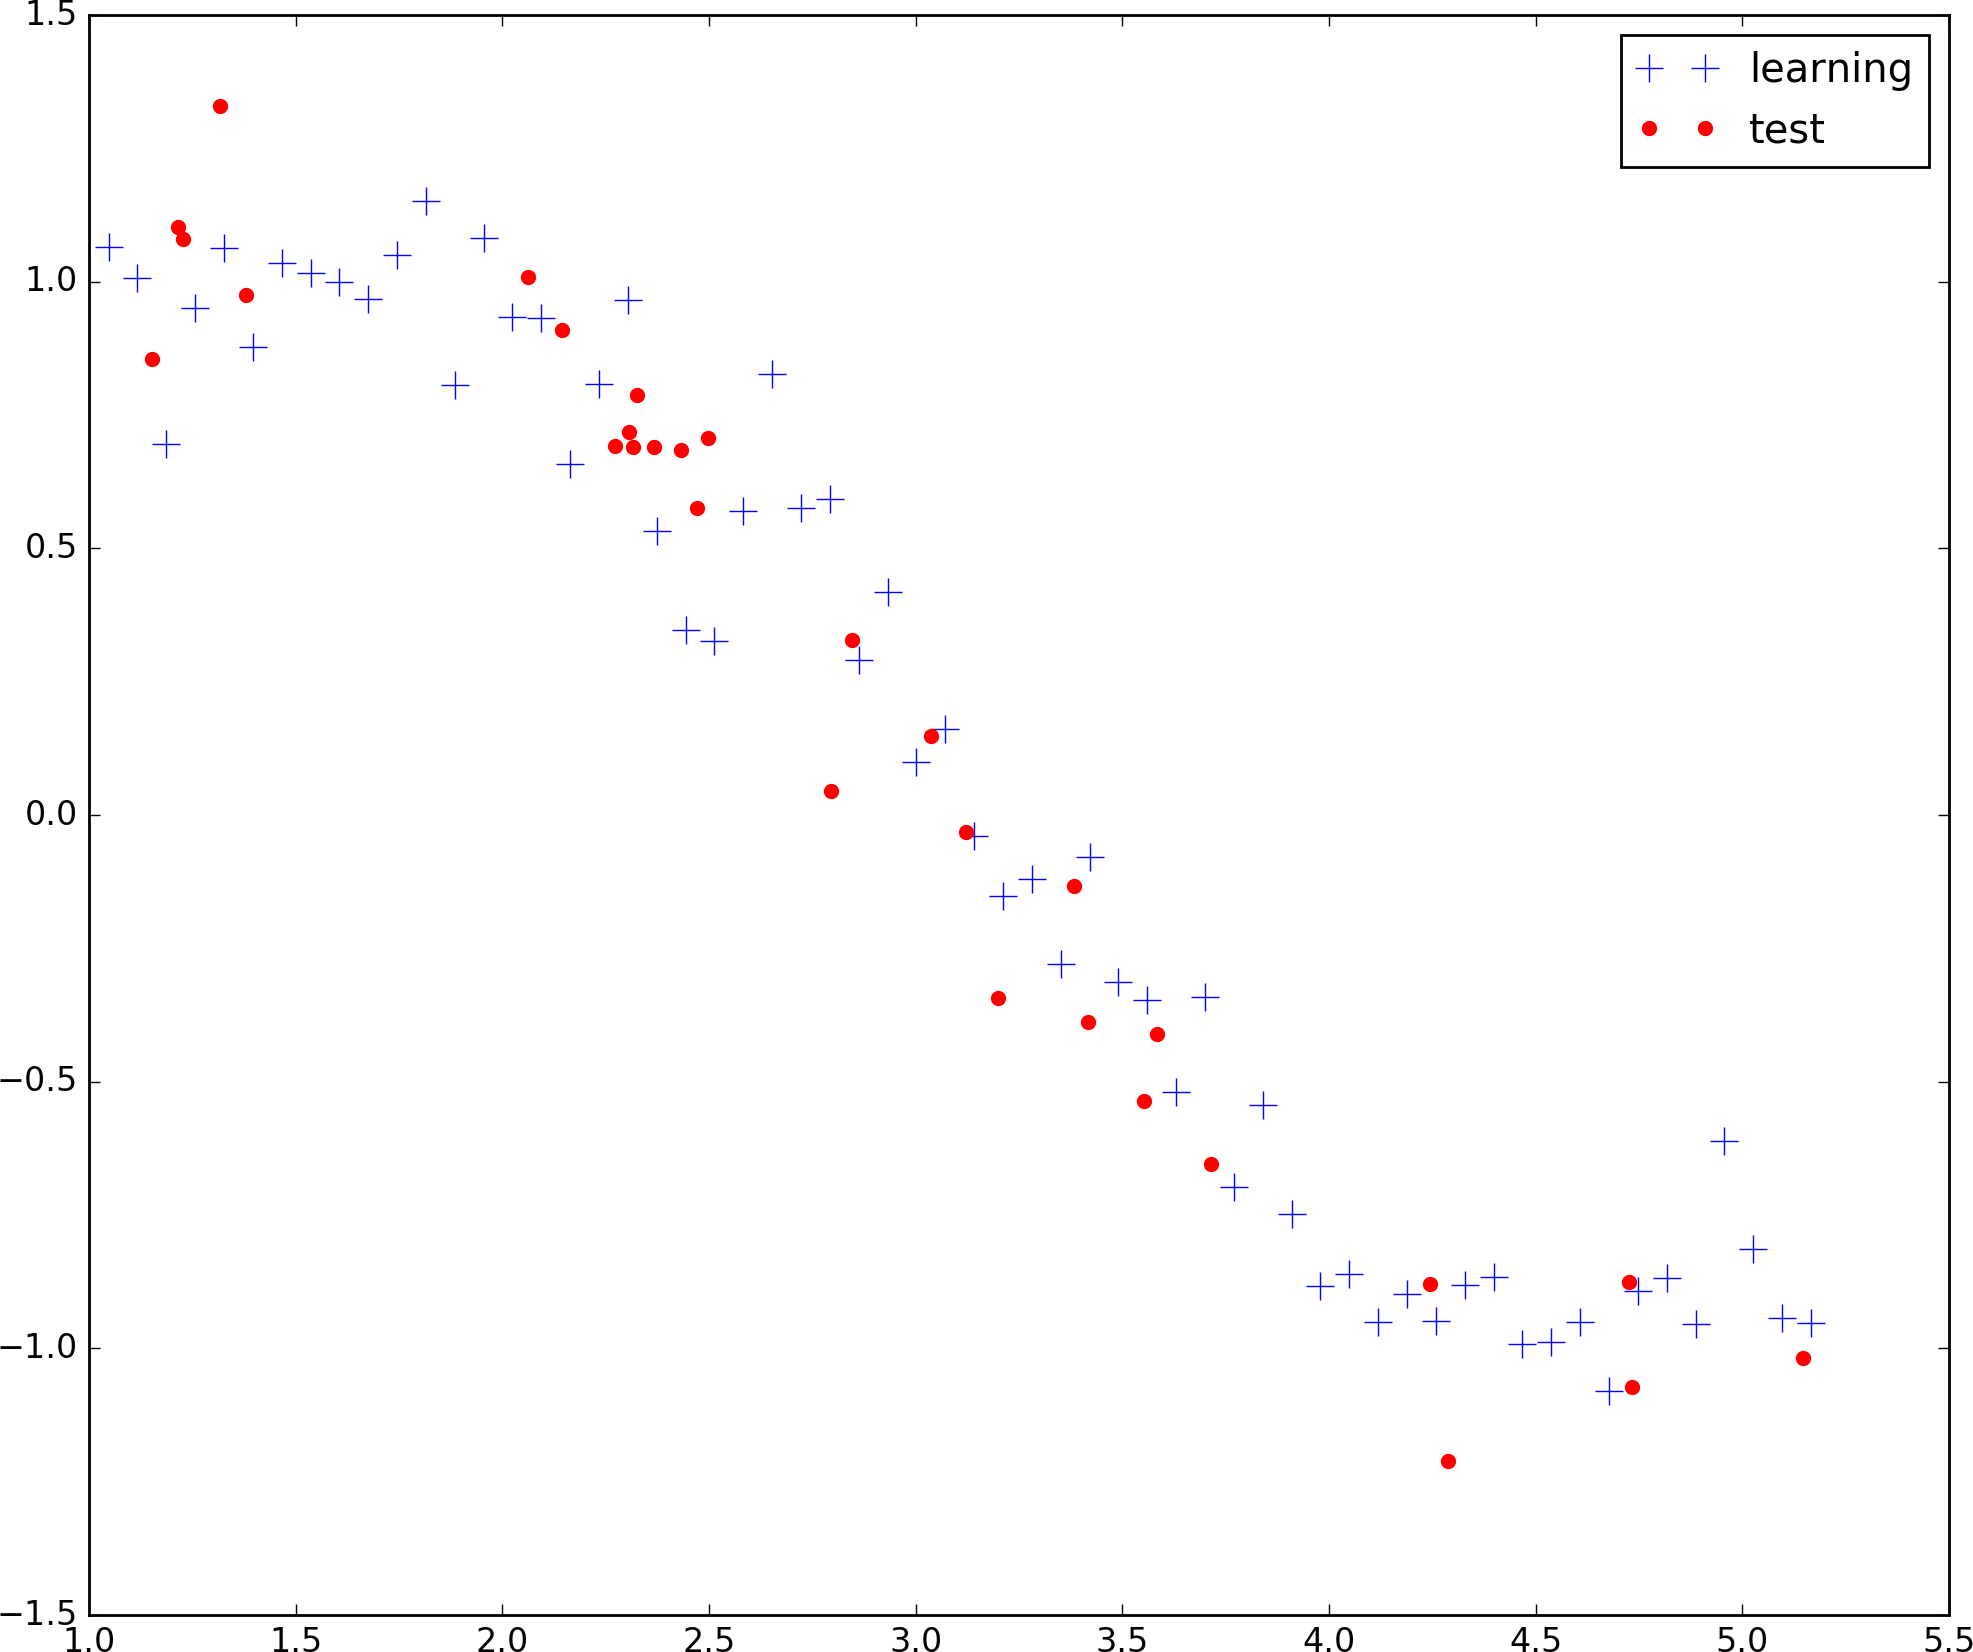
\includegraphics[width=\textwidth]{./fig/scatter_test.png}
\end{figure}
\pause
\column{.5\textwidth}
\begin{figure}
Error on the training and the test
with respect with $\alpha$
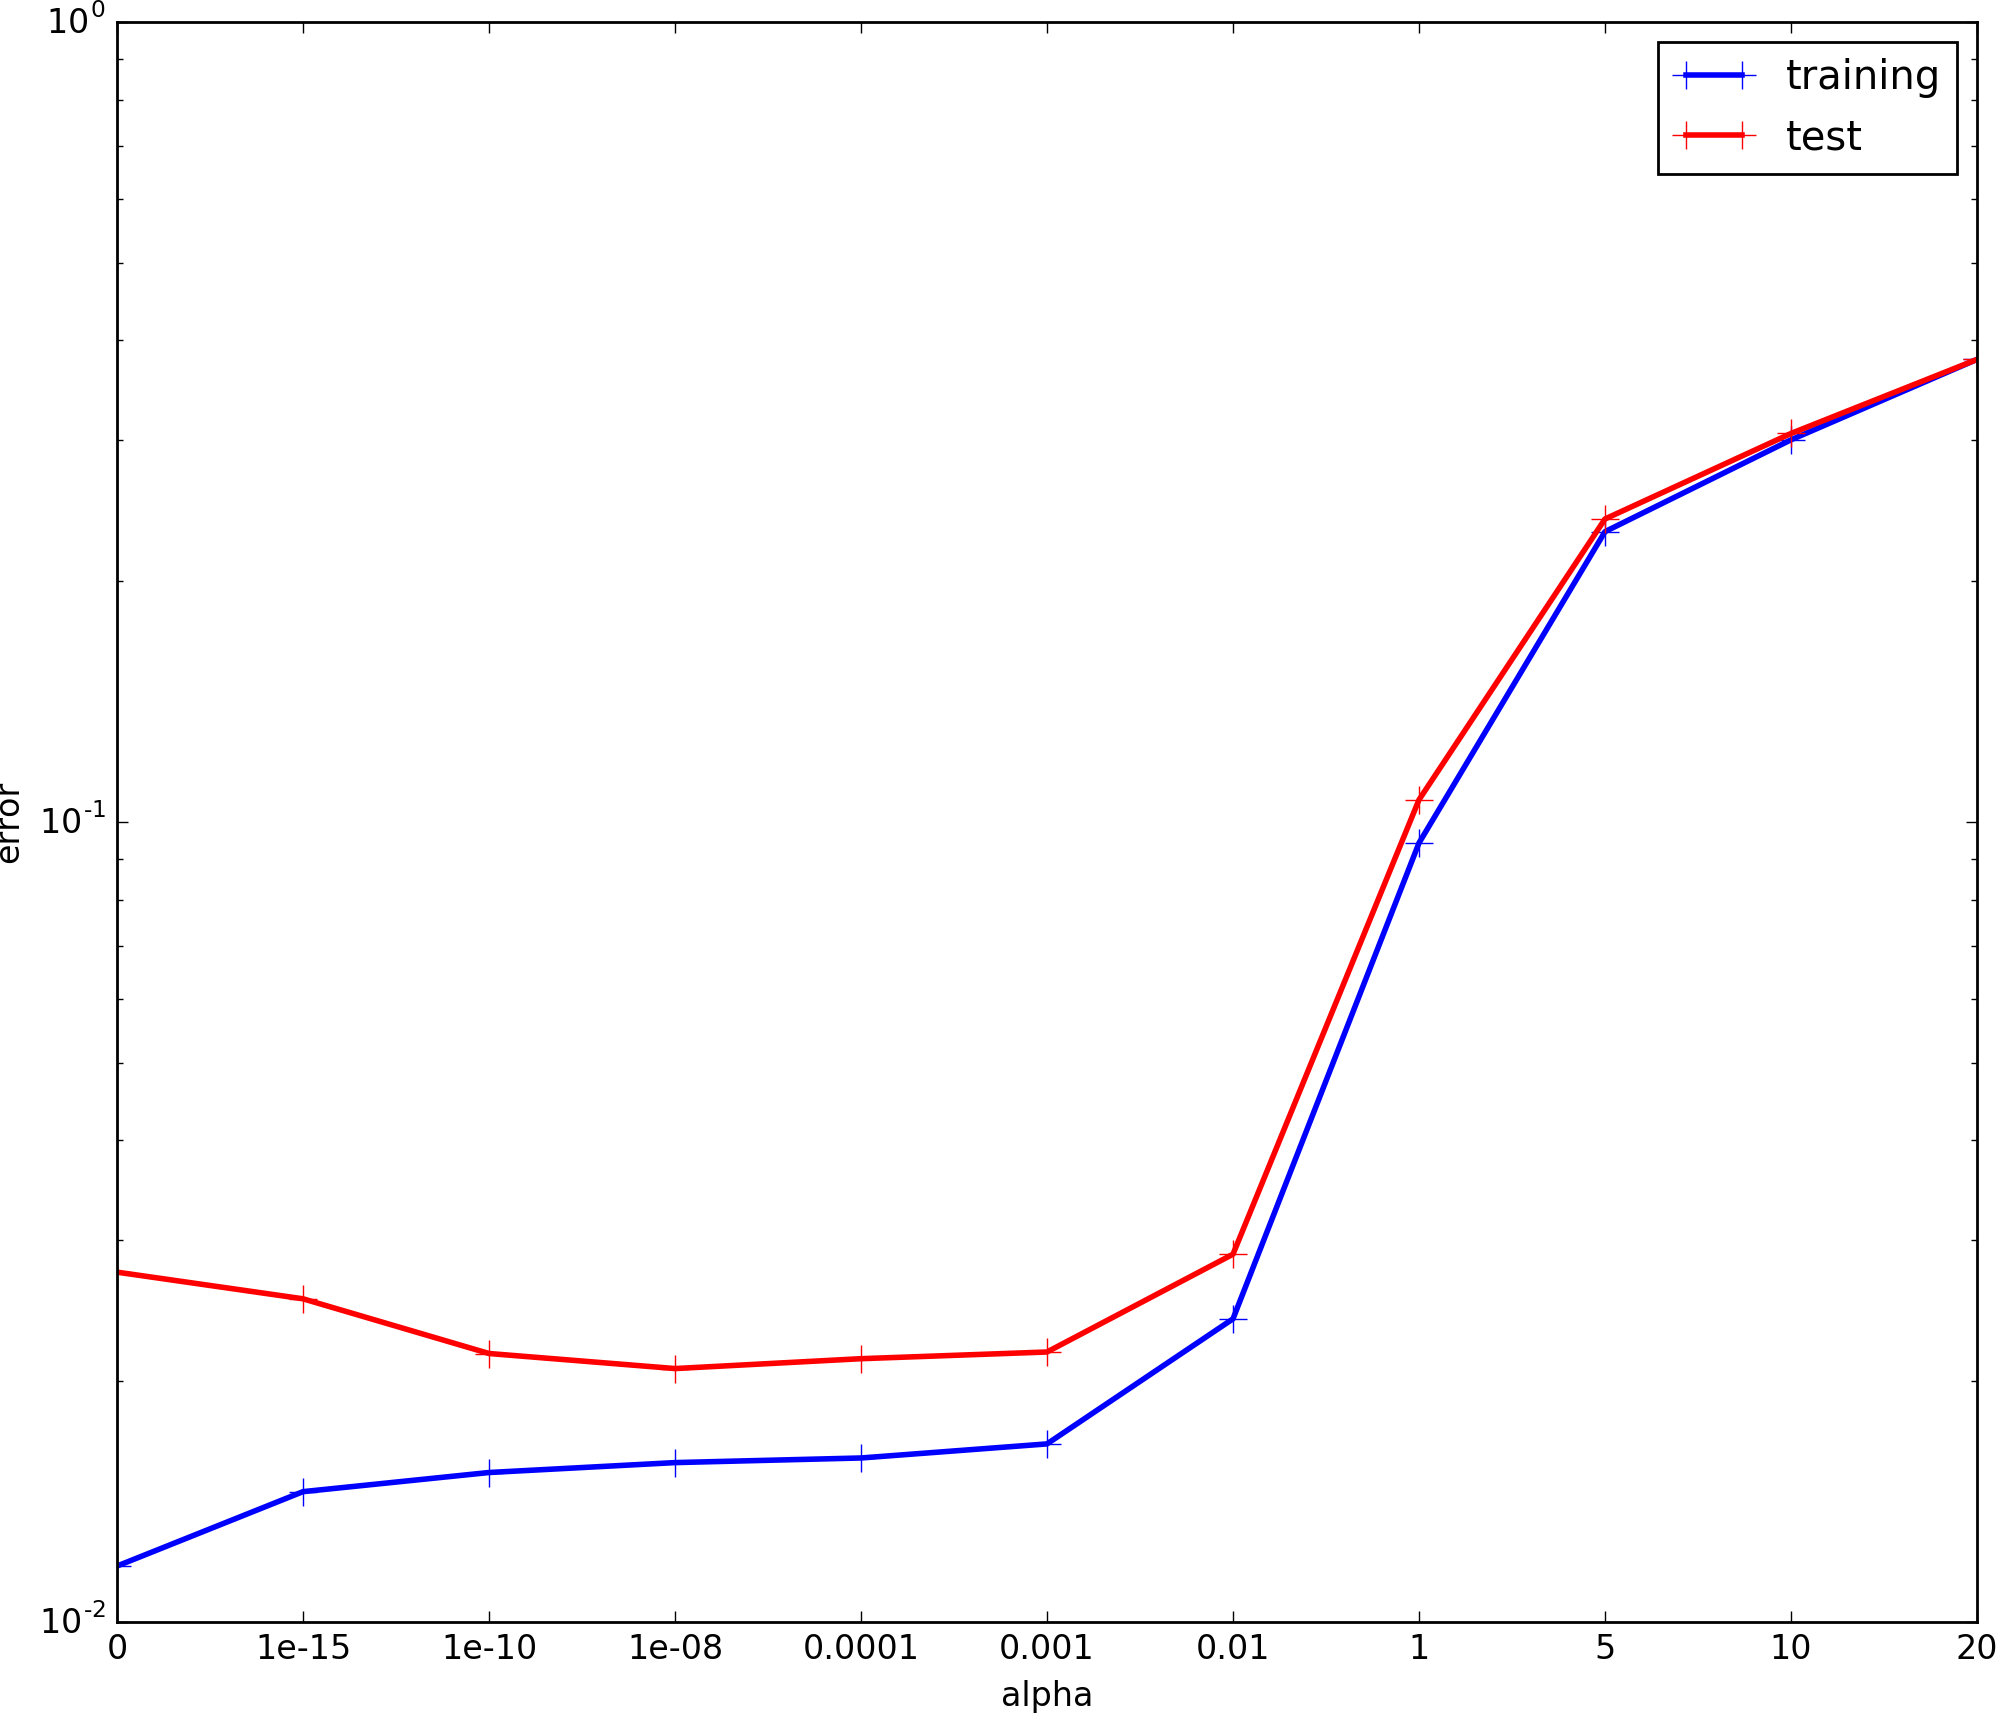
\includegraphics[width=\textwidth]{./fig/validation.png}
\end{figure}

\end{columns}
\end{frame}



\begin{frame}
  \frametitle{Introduction to the percpetron}
  \begin{figure}
  \begin{tikzpicture}[
    basic/.style={draw,fill=blue!20,text width=1em,text badly centered},
    input/.style={basic,circle},
    weights/.style={basic,rectangle},
functions/.style={basic,circle,fill=blue!10},
]
        \node[functions] (center) {};
        \node[below of=center,font=\scriptsize,text width=4em] {Activation function};
        \draw[thick] (0.5em,0.5em) -- (0,0.5em) -- (0,-0.5em) -- (-0.5em,-0.5em);
      %  \draw (0em,0.75em) -- (0em,-0.75em);
      %  \draw (0.75em,0em) -- (-0.75em,0em);
        \node[right of=center, anchor = west] (right) {$y=$ 0 ou 1};
            \path[draw,->] (center) -- (right);
        \node[functions,left=3em of center] (left) {$\sum$};
            \path[draw,->] (left) -- (center);
%        \node[weights,left=3em of left] (2) {$w_2$} -- (2) 
            \node[input,left= 4em of left] (l2) {$x_2$};
%            \path[draw,->] (l2) -- (2);
            \path[draw,->] (l2) -- node[above,midway]{$w_2$}(left);
        \node[below of=l2] (dots) {$\vdots$} ;
%(dots) node[left of=dots] (ldots) {$\vdots$};
%        \node[weights,below of=dots] (n) {$w_n$} -- (n) 
\node[input,below of=dots] (ln) {$x_n$};
%            \path[draw,->] (ln) -- (n);
            \path[draw,->] (ln) -- node[above,midway]{$w_n$}(left);
%        \node[weights,above of=2] (1) {$w_1$} -- (1) 
            \node[input,above of=l2] (l1) {$x_1$};
%            \path[draw,->] (l1) -- (1);
            \path[draw,->] (l1) -- node[above,midway]{$w_1$}(left);
%        \node[weights,above of=1] (0) {$w_0$} -- (0) 
\node[input,above of=l1] (l0) {$1$};
%            \path[draw,->] (l0) -- (0);
            \path[draw,->] (l0) -- node[above,midway]{$w_0$}(left);
        \node[below of=ln,font=\scriptsize](lin) {inputs};
        \node[right of=lin,font=\scriptsize] {weights};
    \end{tikzpicture}
    \end{figure}
\begin{block}{}
If $w_0 + w_1 x_1 + w_2 x_2 +  \dots + w_n\ x_n < 0$, then $y=0$\\
else $y=1$
\end{block}
\end{frame}
\begin{frame}
\frametitle{Two different predictions}

\begin{columns}
\column{0.45\textwidth}
$w_0=$ \red{1}, $w_1=$ \red{-2},$w_2=$ \red{2}\\
\vspace{1em}

 \begin{tikzpicture}[
    basic/.style={draw,fill=blue!20,text width=1em,text badly centered},
    input/.style={basic,circle, text width=1em, inner sep=0},
    weights/.style={basic,rectangle},
functions/.style={basic,circle,fill=blue!10},
]
        \node[functions] (center) {};
        \draw[thick] (0.5em,0.5em) -- (0,0.5em) -- (0,-0.5em) -- (-0.5em,-0.5em);
        \node[right = 1em of center, anchor = west] (right) {$y=$ \red{1}};
            \path[draw,->] (center) -- (right);
        \node[functions,left=1em of center] (left) {$\sum$};
            \path[draw,->] (left) -- (center);
            \node[left= 2em of left] (l2) {$x_1=0$};
            \path[draw,->] (l2) -- node[above,midway]{$w_1$}(left);
            \node[below of=l2] (ln) {$x_2=1$};
            \path[draw,->] (ln) -- node[above,midway]{$w_2$}(left);
            \node[above of=l2] (l1) {$1$};
            \path[draw,->] (l1) -- node[above,midway]{$w_0$}(left);
           % \node[input,above of=l1] (l0) {$1$};
           % \path[draw,->] (l0) -- node[above,midway]{$w_0$}(left);
%        \node[below of=ln,font=\scriptsize](lin) {inputs};
%        \node[right of=lin,font=\scriptsize] {weights};
    \end{tikzpicture}

$$
w_0 + w_1 x_1 + w_2 x_2 = 3 > 0
$$

\column{0.45\textwidth}
$w_0=$ \red{1}, $w_1=$ \red{2},$w_2=$ \red{-2}\\
\vspace{1em}

 \begin{tikzpicture}[
    basic/.style={draw,fill=blue!20,text width=1em,text badly centered},
    input/.style={basic,circle, text width=1em, inner sep=0},
    weights/.style={basic,rectangle},
functions/.style={basic,circle,fill=blue!10},
]
        \node[functions] (center) {};
        \draw[thick] (0.5em,0.5em) -- (0,0.5em) -- (0,-0.5em) -- (-0.5em,-0.5em);
        \node[right = 1em of center, anchor = west] (right) {$y=$ \red{0}};
            \path[draw,->] (center) -- (right);
        \node[functions,left=1em of center] (left) {$\sum$};
            \path[draw,->] (left) -- (center);
            \node[left= 2em of left] (l2) {$x_1=0$};
            \path[draw,->] (l2) -- node[above,midway]{$w_1$}(left);
            \node[below of=l2] (ln) {$x_2=1$};
            \path[draw,->] (ln) -- node[above,midway]{$w_2$}(left);
            \node[above of=l2] (l1) {$1$};
            \path[draw,->] (l1) -- node[above,midway]{$w_0$}(left);
           % \node[input,above of=l1] (l0) {$1$};
           % \path[draw,->] (l0) -- node[above,midway]{$w_0$}(left);
%        \node[below of=ln,font=\scriptsize](lin) {inputs};
%        \node[right of=lin,font=\scriptsize] {weights};
    \end{tikzpicture}

$$
w_0 + w_1 x_1 + w_2 x_2 = -1 < 0
$$

\end{columns}


\end{frame}


\end{document}